\documentclass{article}
\usepackage{graphicx} % Required for inserting images


\usepackage{amsmath}
\usepackage{mathrsfs}
\usepackage{bbm}
\usepackage{hyperref}
\usepackage{amsthm}
\usepackage{amssymb}
\usepackage{tikz}
\usepackage{natbib}
\usetikzlibrary{arrows.meta, positioning, calc, decorations.pathreplacing}


\title{CAPOPM: A Bayesian Hybrid Framework for Derivative Pricing in Behavioral Parimutuel Markets}
\author{Sean Slattery}
\date{November 2025}

\newtheorem{remark}{Remark}
\newtheorem{lemma}{Lemma}
\newtheorem{theorem}{Theorem}
\newtheorem{prop}{Proposition}
\newtheorem{corollary}{Corollary}
\newtheorem{assumption}{Assumption}
\newtheorem{definition}{Definition}

\begin{document}

\maketitle



\begin{abstract}
This paper develops CAPOPM, a crowd-adjusted parimutuel option pricing 
mechanism that integrates structural financial models, machine learning forecasts, and trader behavior
forecasting, and trader behavior within a unified Bayesian framework.  
Rather than treating derivative prices as primitives or relying solely on 
structural models, CAPOPM views trader actions in a parimutuel setting as 
yielding a hybrid prior that balances neutrality with data\u2011driven predictive content. The second stage introduces structural corrections for liquidity imbalances or whale dominance.
Both adjustments are designed to preserve Beta--Binomial conjugacy, enabling 
closed-form posteriors while allowing the model to represent several sources of 
distortion present in real markets.

The resulting posterior distribution over event probabilities can be viewed as 
an interpretable belief-extraction mechanism.  Phase~7 examines the empirical 
properties of this mechanism through simulation, including stress tests for 
herding and correlated behavior.  Phase~8 provides theoretical analysis, 
showing that under reasonable assumptions and bounded distortions, the 
posterior is robust, consistent, and asymptotically normal as the effective 
sample size grows.

The goal of this work is not to claim empirical dominance or to present a 
fully calibrated pricing engine, but to establish a structured approach for 
combining structural finance, machine learning, and crowd behavior into a 
coherent Bayesian updating procedure.  CAPOPM is proposed as a flexible 
foundation that can be extended, calibrated, and empirically validated in a 
variety of market environments.

\end{abstract}


\section{Introduction}

\subsection{Background and Motivation}

Modern derivative markets bring together structural 
% --- Refactored CAPOPM sections inserted below ---
% Legacy content moved to paper/prism/_legacy/phase1_refactor.tex

%% Phase  2 refactor: Hybrid prior fusion under flat assumptions

\subsection{Phase~2: Hybrid Prior Fusion}\label{sec:phase2-hybrid}

In the refactored CAPOPM framework the hybrid prior fuses the non‑informative structural prior from Phase~1 with a principled machine‑learning (ML) prior.  This fusion encodes both epistemic humility and data‑driven insight while preserving the analytic convenience of conjugate Beta distributions.

\begin{definition}[Hybrid prior via product of Beta distributions]\label{def:hybrid-prior-product}
Let $p$ denote the event probability, and let the structural and ML priors be defined as in Definitions~\ref{def:structural-prior-flat} and~\ref{def:ml-prior}.  We assume these two sources of belief are independent, so the joint prior density factors as
\[
  f(p) \;\propto\; f_{\text{structural}}(p)\,f_{\text{ML}}(p).
\]
Since both factors are Beta densities, their product is proportional to another Beta density.  In particular,
\begin{equation}\label{eq:beta-product}
  f_{\text{hybrid}}(p)
  \propto p^{(1-1)+(\alpha_{\mathrm{ML}}-1)}\,(1-p)^{(1-1)+(\beta_{\mathrm{ML}}-1)}
  = p^{\alpha_{\mathrm{ML}}-1}\,(1-p)^{\beta_{\mathrm{ML}}-1},
\end{equation}
so the hybrid prior is the Beta distribution
\[
  p \sim \operatorname{Beta}(\alpha_{\mathrm{ML}},\beta_{\mathrm{ML}}).
\]
This result reflects the fact that a flat $\operatorname{Beta}(1,1)$ structural prior contributes zero pseudo‑observations (see Remark~\ref{rem:pseudo}), leaving the ML pseudo‑counts $(\alpha_{\mathrm{ML}},\beta_{\mathrm{ML}})$ unchanged.
\end{definition}

\begin{remark}[Pseudo‑sample interpretation]\label{rem:pseudo}
For a Beta distribution $\operatorname{Beta}(\alpha,\beta)$ one can interpret $(\alpha-1)$ and $(\beta-1)$ as the numbers of prior ``success'' and ``failure'' observations, respectively.  A flat structural prior has $\alpha = \beta = 1$, corresponding to zero pseudo‑observations.  Thus the product \eqref{eq:beta-product} simply recovers the ML prior $\operatorname{Beta}(\alpha_{\mathrm{ML}},\beta_{\mathrm{ML}})$: the structural prior anchors the domain but does not contribute additional information.  When $n_{\mathrm{eff}}=0$ in Definition~\ref{def:ml-prior}, the hybrid prior collapses to $\operatorname{Beta}(1,1)$.
\end{remark}

\begin{lemma}[Hybrid posterior update]\label{lem:hybrid-posterior}
Under Assumption~\ref{assump:parimutuel-likelihood} and Definition~\ref{def:hybrid-prior-product}, the posterior distribution of $p$ after observing $y'$ effective YES bets and $n' - y'$ effective NO bets is
\[
  p \mid y' \sim \operatorname{Beta}(\alpha_{\mathrm{ML}} + y',\,\beta_{\mathrm{ML}} + n' - y').
\]
In other words, the flat structural prior does not alter the Beta--Binomial update beyond the pseudo--counts contributed by the ML prior.  This follows directly from the conjugate update $\alpha' = \alpha + y'$ and $\beta' = \beta + n' - y'$ for a Beta--Binomial model \cite{Data140_Updating}.\end{lemma}
\pa%ragraph{Parameterization by mean and effective sample size.}
The ML prior $\operatorname{Beta}(\alpha_{\mathrm{ML}},\beta_{\mathrm{ML}})$ can be parameterized by its mean $\mu$ and effective sample size $n_{\mathrm{eff}}$ via $\alpha_{\mathrm{ML}} = \mu\,n_{\mathrm{eff}}$ and $\beta_{\mathrm{ML}} = (1-\mu)\,n_{\mathrm{eff}}$. Equivalently, if $\mu$ and $\nu = \alpha_{\mathrm{ML}} + \beta_{\mathrm{ML}}$ denote the mean and ``sample size'' of a Beta distribution, then $\alpha = \mu \, \nu$ and $\beta = (1-\mu)\nu$. This parameterization clarifies how the prior mean anchors the distribution while $n_{\mathrm{eff}}$ controls its concentration. In the hybrid prior, this interpretation persists because the structural prior contributes no additional pseudo\,observations.
\paragraph{Discussion and implications.}
The hybrid prior fusion emphasises that CAPOPM’s belief state is the product of an epistemically neutral structural anchor and a data‑driven ML component.  By adopting $\operatorname{Beta}(1,1)$ as the structural prior, we ensure that the hybrid prior is entirely determined by the ML pseudo‑counts.  This design maintains conjugacy with the parimutuel likelihood and preserves interpretability.  We stress that structural complexity, such as stochastic volatility models, can still inform the ML prior (e.g., via a model‑based forecast mean and variance), but it no longer functions as a canonical generator of dynamics.  Consequently, the proofs and propositions that relied on fractional Heston dynamics in the original draft either reduce to statements about optional modules or become vacuous under the flat prior.

% Legacy content moved to paper/prism/_legacy/phase3_parimutuel_mechanism.tex

%% Phase 6 refactor: Behavioral and structural corrections

\subsection{Phase~6: Behavioral and Structural Corrections}\label{sec:phase6-corrections}

The predictive accuracy of a parimutuel market depends not only on the prior distribution and the mechanism for aggregating information, but also on the quality of the input signals.  Real‑world bettors exhibit systematic biases such as the favourite–longshot bias, herding and overconfidence.  Moreover, structural features of the market—liquidity imbalances or large strategic orders—can distort the relationship between raw order flow and underlying beliefs.  Phase 6 introduces corrections that map raw YES/NO counts to effective counts $(y',n')$ for use in the Beta–Binomial update.  These corrections are essential in the refactored framework because the flat structural prior places greater weight on early data; failure to adjust for biases could lead to severely skewed posteriors.

%The favourite--longshot bias is the empirical regularity that bets placed at higher offered odds (longshots) yield worse rates of return than bets placed at lower odds (favourites). In traditional betting markets this bias manifests as systematic overpricing of longshot contracts relative to their true probabilities. To correct for this bias, CAPOPM applies a transformation $y \mapsto y' = f(y)$ that down-weights longshot orders and up-weights favourite orders according to a calibrated function $f$.\end{definition}
\end{definition}

\begin{definition}[Herding correction]\label{def:herding}
Herd behavior refers to individuals acting collectively without centralized direction\citeLeadershipIQ_Herding.  In prediction markets, herding can manifest when traders mimic the actions of others rather than relying on their private information.  To mitigate herding, CAPOPM applies a dampening function $g$ to clusters of identical orders arriving in quick succession, thereby reducing the effective weight of copycat trades while preserving genuinely independent signals.
\end{definition}

\begin{definition}[Structural corrections]\label{def:structural-correction}
Structural corrections address market frictions such as liquidity imbalances or the presence of large, possibly strategic orders.  For instance, if a single large trader places a block order, the raw count $n$ may overstate the amount of independent information.  A structural correction $h$ maps $(y,n)$ to $(y'',n'')$ by capping the influence of any one participant and by normalizing counts across liquidity regimes.  In the refactored framework structural corrections are modular: they may incorporate optional models of market depth or order‑book dynamics, but they do not introduce additional stochastic processes into the prior.
\end{definition}

\begin{assumption}[Monotonicity and invariance]\label{assump:corrections}
The correction functions $f$, $g$ and $h$ are assumed to be deterministic, monotonic and time‑invariant.  They preserve order (if $y_1 \le y_2$ then $f(y_1) \le f(y_2)$) and depend only on observable order‑flow statistics.  Corrections are applied sequentially: first behavioural corrections (favourite–longshot and herding), followed by structural corrections.  The resulting effective counts $(y',n')$ enter the Beta–Binomial update described in Phase~3.
\end{assumption}

\begin{lemma}[Posterior with corrections]\label{lem:correction-posterior}
Let $p \sim \operatorname{Beta}(\alpha_{\mathrm{ML}},\beta_{\mathrm{ML}})$ be the hybrid prior from Phase~2 and suppose raw YES and NO counts $(y,n-y)$ are transformed to $(y',n'-y')$ via behavioural and structural corrections satisfying Assumption~\ref{assump:corrections}.  Then, under the Binomial model $y' \mid p \sim \operatorname{Binomial}(n',p)$, the posterior distribution of $p$ is
\[
  p \mid y' \sim \operatorname{Beta}(\alpha_{\mathrm{ML}} + y',\; \beta_{\mathrm{ML}} + n' - y').
\]
The corrections enter only through the adjusted counts, leaving the functional form of the posterior unchanged.
\end{lemma}

\begin{remark}[Calibration challenges]
The choice of correction functions $f$, $g$ and $h$ introduces additional hyperparameters that must be calibrated empirically.  In the original CAPOPM implementation these calibrations relied on stress tests and simulations.  Under the flat prior, improper calibration can have a more pronounced impact because there is less regularization from structural dynamics.  It is therefore essential to validate corrections using historical data and out‑of‑sample evaluation.
\end{remark}

\paragraph{Discussion.}
Behavioural and structural corrections play a central role in extracting meaningful information from noisy order flow.  By explicitly modelling common biases—favourite–longshot, herding and strategic trading—the CAPOPM framework produces effective counts that better reflect independent beliefs.  These corrected counts feed into the Beta–Binomial update, preserving analytic tractability.  While our refactoring demotes stochastic volatility models to optional modules, it reaffirms the importance of robust correction schemes and highlights the sensitivity of posteriors to early data under a flat structural prior.

% Legacy content moved to paper/prism/_legacy/phase7_simulations.tex

% Legacy content moved to paper/prism/_legacy/phase8_theoretical_results.tex

% Literature Review and Conclusion for CAPOPM
% This section completes the refactor by aligning the literature review
% and concluding remarks with the flat prior framework.  It omits detailed
% discussions of fractional Heston dynamics and instead highlights work on
% conjugate priors, Beta–Binomial models, and parimutuel markets.

\section{Literature Review}

The original CAPOPM paper surveyed a broad range of financial models,
including fractional Heston processes, stochastic volatility models, and
non‑parametric machine learning approaches.  In the simplified version we
restrict attention to models that are relevant to the flat‑prior, Beta–Binomial
framework and to parimutuel prediction markets.

\paragraph{Bayesian inference for binary events.}  Bayesian analysis of
binary outcomes typically employs the Beta distribution as a conjugate prior
for the Bernoulli or binomial likelihood.  This choice dates back to the
classical works of Laplace and remains a cornerstone of modern Bayesian
statistics.  The Beta distribution \(\operatorname{Beta}(a,b)\) has a tractable
posterior update when combined with binomial data: if \(p\) has prior
\(\operatorname{Beta}(a,b)\) and \(y\) successes are observed in \(n\)
trials, the posterior is \(\operatorname{Beta}(a+y,b+n-y)\)\cite{714310495055200}.  Its mean is
\(a/(a+b)\) and its variance is \(ab/((a+b)^2(a+b+1))\)\cite{315913489390355}, allowing
closed‑form expressions for posterior summaries.

\paragraph{Prediction markets and parimutuel mechanisms.}  Prediction markets
and parimutuel betting schemes aggregate information by letting traders buy
shares contingent on outcomes.  Market prices in a pari‑mutuel market with
binary events can be interpreted as estimates of the event probability and
provide a natural likelihood for Bayesian updating.  Studies by
\citet{wolfers2004prediction} and \citet{manski2006interpreting} argue that
market prices approximate subjective probabilities when participants are
risk‑neutral and face no liquidity constraints.  More recent research
investigates behavioural biases (e.g., favourite–longshot bias) in sports
betting\cite{609924582939380} and herding phenomena in financial markets\cite{619800483002449}, which motivate the
correction functions introduced in Phase 6.

\paragraph{Conjugate priors in machine learning.}  Machine learning models
often produce point forecasts without quantified uncertainty.  To incorporate
such forecasts into Bayesian decision making, one can construct a principled
Beta prior by specifying a forecast mean \(\mu\) and an effective sample size
\(n_{\mathrm{eff}}\).  This parameterization, also known as the method of
moments, sets \(\alpha=\mu n_{\mathrm{eff}}\) and
\(\beta=(1-\mu)n_{\mathrm{eff}}\).  The resulting Beta prior reflects both
the point estimate and the confidence level of the machine learning model.

\paragraph{Hybrid Bayesian frameworks.}  Combining structural and empirical
priors is common in modern Bayesian econometrics.  The CAPOPM framework
belongs to this family: it fuses a non‑informative structural prior
\(\operatorname{Beta}(1,1)\) with a principled ML prior via independent
products.  Similar ideas appear in works on hierarchical modelling and
empirical Bayes, where prior hyperparameters are estimated from data.

\section{Conclusion}

The refactored CAPOPM framework provides a simplified yet rigorous foundation
for belief aggregation in parimutuel prediction markets.  By adopting a
flat \(\operatorname{Beta}(1,1)\) structural prior, CAPOPM eliminates
unjustified complexity from fractional Heston dynamics and focuses on
information extraction and behavioural correction.  The hybrid prior,
constructed as a product of the flat prior and a principled machine–learning
\(\operatorname{Beta}(\alpha_{\mathrm{ML}},\beta_{\mathrm{ML}})\) prior, yields
a conjugate \(\operatorname{Beta}(\alpha_{\mathrm{ML}},\beta_{\mathrm{ML}})\)
distribution for the event probability.  Posterior updates follow the
Beta–Binomial conjugacy, allowing closed‑form expressions for the mean and
variance and straightforward integration of effective order‑flow counts.

The theoretical analysis demonstrates that CAPOPM is consistent and
asymptotically normal under mild conditions (Phase 8), and the simulation
studies (Phase 7) highlight the trade‑offs introduced by the effective sample
size and behavioural corrections.  The modular design of the framework
accommodates optional structural layers, such as stochastic volatility, but does
not require them for validity.

Looking forward, future work can explore empirical calibration of the machine
learning prior, incorporate richer behavioural models, and extend the framework
to multi‑outcome events.  While the present formulation avoids overfitting by
maintaining epistemic humility, it remains a flexible platform for research on
prediction markets, information aggregation, and Bayesian mechanism design.



financial models, 
algorithmic trading systems, and heterogeneous crowds of participants, each 
possessing partial or noisy information.  As quantitative methods have 
advanced, two broad approaches to pricing derivatives have emerged.  
The first centers on structural asset dynamics, using stochastic volatility 
models and their extensions to obtain risk-neutral prices.  
The second leverages machine learning algorithms, which are trained directly 
on historical data to approximate option prices or event probabilities.  
Both approaches are powerful, but each is limited in isolation: structural 
models may be rigid or miscalibrated in volatile markets, while machine 
learning methods lack interpretability and can behave unpredictably outside 
their training regimes.

In parallel to these developments, parimutuel prediction markets and 
crowd-based financial platforms have shown that aggregate order flow can 
encode meaningful information about uncertain outcomes.  When participants act 
on private signals or interpretations of public news, their trades generate a 
rich stream of behavioral and informational content.  Yet this information is 
rarely integrated into option pricing models in a principled way.  
The goal of this paper is to explore a mechanism through which such crowd 
signals, structural models, and machine learning outputs can be combined 
through a Bayesian framework.

\subsection{Challenges in Existing Approaches}

Approaches to belief aggregation and pricing often assume clean separation 
between trader behavior, structural assumptions, and statistical estimation.  
Structural models depend heavily on parameter calibration and may struggle 
under regime changes.  Machine learning methods can fit historical data well 
but typically provide point estimates without uncertainty quantification.  
Prediction markets aggregate information but do not easily interface with 
risk-neutral pricing or structural modeling.

Behavioral biases further complicate the picture.  
Long-shot bias, correlated trading, herding cascades, and liquidity asymmetry 
can distort raw order flow.  Without a systematic way to adjust for these 
effects, trader actions cannot be directly interpreted as signals about future 
prices or event probabilities.  
Additionally, existing Bayesian updating frameworks rely on conditional 
independence, an assumption that breaks down in settings where trader behavior 
is reactive or networked.

These challenges motivate a framework that (i) integrates structural and 
machine learning priors, (ii) preserves interpretability, (iii) incorporates 
behavioral and structural corrections, and (iv) provides theoretical guarantees 
under realistic assumptions.

\subsection{Literature Review}

A number of strands of research motivate the CAPOPM framework.  
First, the tempered fractional Heston model of Shi~\cite{Shi} introduces a volatility
process with fractional memory through a Riccati--Volterra system, offering a 
generalization of classical stochastic volatility while retaining 
exponential-affine structure useful for option pricing.  
This model forms the structural component of the CAPOPM prior.

Second, work by Koessler, Noussair, and Ziegelmeyer~\cite{KoesslerNoussairZiegelmeyer} examines information
aggregation in parimutuel betting markets under asymmetric information.  
Their analysis demonstrates that trader participation and signal structure 
influence market-clearing probabilities in systematic ways.  
This literature informs the representation of trader actions as information 
signals within CAPOPM.

Third, Axelrod, Kulick, Plott, and Roust~\cite{AxelrodPlott} develop mechanisms to improve 
parimutuel-type aggregation, addressing inefficiencies such as long-shot bias 
and disequilibrium phenomena.  
Their results motivate the need for behavioral adjustments before interpreting 
order flow as informational.

A separate line of work, represented by D'Uggento, Biancardi, and 
Ciriello~\cite{DUggento2025}, investigates machine learning approaches for 
pricing derivatives and predicting option prices.  
  
Their findings show that neural network models can capture nonlinearities that 
structural models miss, though such models require careful interpretation due 
to uncertainty and generalization limits.

Beyond these core sources, the broader literature on prediction markets, 
behavioral biases, and market microstructure provides context.  
Prediction markets demonstrate that crowds can aggregate dispersed private 
signals, especially when incentives are aligned.  
Behavioral finance research documents systematic distortions in participant 
behavior, including overreaction, herding, and asymmetry in risk perception.  
Finally, microstructure models highlight how liquidity imbalances, strategic 
trading, and asymmetric information influence observable order flow.

CAPOPM draws from each of these areas, but its primary novelty lies in 
integrating them into a single Bayesian mechanism for belief extraction.

\subsection{Overview of the CAPOPM Framework}

.CAPOPM is organized into an eight-phase structure. Flat $\mathrm{Beta}(1,1)$ structural prior and a principled ML Beta prior parameterized by the forecast mean and effective sample size serve as belief anchors. These priors are fused via a pseudo-sample interpretation to form a hybrid prior distribution for the event probability $p$ while preserving Beta--Binomial conjugacy. This hybrid prior is then corrected for behavioral effects (e.g., herding, long-shot bias) and structural distortions (e.g., liquidity imbalances). The adjusted likelihood is combined with the hybrid prior to produce a posterior distribution. Simulation regimes are used to study how the posterior behaves under dependence, correlated trading, and other deviations from model assumptions. Phase~8 provides theoretical results showing that the posterior is robust to bounded distortions and concentrates near the true probability under fairly mild conditions.
The adjusted likelihood is combined with the hybrid prior to produce a 
model assumptions.  
Phase~8 provides theoretical results showing that the posterior is robust to 
bounded distortions and concentrates near the true probability under fairly 
mild conditions.

\subsection{Contributions and Novelty}

While CAPOPM draws on ideas from structural option pricing, machine learning forecasting, and parimutuel information aggregation, its primary contribution lies in organizing these elements into a coherent belief-updating framework. The approach developed here differs from existing models in three main respects. First, a flat $\mathrm{Beta}(1,1)$ structural prior and a principled ML Beta prior parameterized by the forecast mean and effective sample size are combined via a pseudo-sample interpretation; this provides a transparent way to balance epistemic neutrality with data-driven signals. Second, parimutuel order flow is modeled through a two-stage adjustment that accounts for behavioral patterns (such as long-shot bias and herding) and structural distortions (such as liquidity), while preserving conjugacy and permitting cross-sectional estimation. Third, the framework is modular: additional structural complexity, such as stochastic volatility models, can be incorporated as optional extensions, and each layer can be examined and stress tested independently.ted independently.

The goal of this paper is not to claim empirical superiority but to establish 
a foundation for a mathematically interpretable belief-extraction mechanism 
that could be applied to derivative markets.  By treating trader actions as 
informational signals updating a hybrid prior, CAPOPM offers a way to study 
how structural models, machine learning outputs, and crowd behavior interact in a setting where probabilities, not prices, are the central object, with 
prices recovered subsequently via the structural prior and pricing kernel.  
The framework is intended as a starting point for further empirical and theoretical 
development rather than a finalized model.


\subsection{Limitations and Scope}

While CAPOPM combines several modeling elements into a unified framework, it 
is not intended as a fully calibrated pricing engine.  
The structural prior inherits sensitivity to the parameterization of the 
fractional Heston model.  
Machine learning predictions require careful tuning and may behave unpredictably 
outside their training domain.  
Behavioral corrections mitigate but do not eliminate distortions from extreme 
herding or low-liquidity conditions.  
Finally, empirical validation is left for future work.

\subsection{Roadmap}

The remainder of the paper is organized as follows.  
Phase~1 develops the structural prior using the tempered fractional Heston 
model.  
Phase~2 constructs the hybrid prior combining structural and machine learning 
components.  
Phase~3 sets out the trader information structure and event definition.  
Phase~4 presents the Bayesian updating mechanism.  
Phase~5 introduces the parimutuel likelihood.  
Phase~6 develops behavioral and structural correction layers.  
Phase~7 conducts simulation analysis under a variety of trader behaviors.  
Phase~8 provides theoretical guarantees on robustness, consistency, and 
asymptotic normality.  
The paper concludes with discussion and avenues for further research.

\noindent
Phase~1 establishes the structural prior for the CAPOPM framework, grounding
the binary event probability in a well--posed stochastic volatility model.
This prior provides the Bayesian anchor for the later fusion of machine
learning predictions and behavioral distortions.


\section*{Phase 1. Structural Prior and Event Foundations}

%%%%%%%%%%%%%%%%%%%%%%%%%%%%%%%%%%%%%%%%%%%%%%%%%%%%%%%%%%%%%%%%%%%%%%%%
\subsection*{0. Notation, Probability Space, and Market Environment}

We work on a filtered probability space
\[
(\Omega,\mathcal{F},(\mathcal{F}_t)_{t\ge0},Q),
\]
where \(Q\) is the risk–neutral measure.
Let \(S_t\) be the underlying asset price, \(V_t\) the variance process, and 
\((W_t,B_t)\) a pair of Brownian motions with correlation \(\rho\in[-1,1]\).
All expectations \(E[\cdot]\) are taken under \(Q\).

\paragraph{Tempered fractional kernel.}
For \(\alpha\in(1/2,1)\) and tempering parameter \(\lambda\ge0\), define
\[
K_{\alpha,\lambda}(t-s)
:= e^{-\lambda (t-s)} (t-s)^{\alpha-1},
\]
as introduced in the tempered–fractional Heston framework of Shi \cite{Shi}.

\noindent
The restriction $\alpha>1/2$ guarantees square--integrability of the kernel,
ensuring that the stochastic convolution in \eqref{eq:V} is well defined
\cite{KaratzasShreve1991,ElEuchRosenbaum2019}.


\paragraph{Well--posedness references.}
The tempered fractional kernel $K_{\alpha,\lambda}$ enters the Volterra SDE for
$V_t$. Existence and uniqueness of the associated stochastic integrals follow
from the general theory of Volterra--type SDEs in 
\cite{Oksendal2003,KaratzasShreve1991}, while the connection to rough--Heston
kernels and their regularity properties is detailed in 
\cite{ElEuchRosenbaum2019}. Shi's construction \cite{Shi} provides the
specialized tempered--fractional case used here.



\paragraph{Event of interest.}
Following the event structure of Koessler, Noussair, and Ziegelmeyer 
\cite{KoesslerNoussairZiegelmeyer}, define the CAPOPM binary state:
\[
A := \{S_T > K\},
\qquad 
A^c := \{S_T \le K\}.
\]
A parimutuel YES contract pays \(1\) if \(A\) occurs and \(0\) otherwise. Following the event framework of Koessler, Noussair, and Ziegelmeyer
\cite{KoesslerNoussairZiegelmeyer}, define the binary CAPOPM terminal event
under the risk--neutral measure $Q$ induced by the structural prior:


\paragraph{Interpretation.}
The binary payoff structure mirrors the experimental parimutuel design of
Koessler, Noussair, and Ziegelmeyer \cite{KoesslerNoussairZiegelmeyer}, where
traders submit YES/NO orders on terminal events. This creates a direct mapping
between the structural prior probability and the parimutuel prior odds used in
later phases of CAPOPM. This matches the parimutuel aggregation mechanism studied by Axelrod, Plott,
and coauthors \cite{AxelrodPlott}, where prices reflect aggregated beliefs on
binary terminal events.




\paragraph{Trader population and private information.}
There are \(N=\{1,\dots,n\}\) traders.  
Trader \(i\) receives a private signal \(\xi_i\in\{H,L\}\) with likelihoods
\[
P(\xi_i = H \mid A)=p,\qquad  
P(\xi_i = H \mid A^c)=1-p,
\]
with $p\in(1/2,1)$. This symmetric specification matches the binary-signal
design used in experimental parimutuel markets
\cite{KoesslerNoussairZiegelmeyer}.


Trader \(i\) selects
\[
s_i\in\{\mathrm{YES},\mathrm{NO}\},
\]
and the full action profile is \(s=(s_1,\dots,s_n)\).

\paragraph{Remark.}
The conditional i.i.d.\ assumption is used only in Phase~1 and is relaxed in
later phases to accommodate dependence (herding), multimodality, and nonlinear
distortions; see \cite{Doukhan1994,Cappe2005}.


\paragraph{Cross–phase notation.}
To prepare for later phases, define:
\[
\pi_{\mathrm{prior}} := Q(S_T>K),\qquad 
L(s\mid A),\quad L(s\mid A^c)
\]
as the parimutuel likelihoods;  
\[
\pi_{\mathrm{post}} := Q(A\mid s)
\]
as the CAPOPM posterior;  
and
\[
\pi_{\mathrm{pred}}
\]
as the posterior–predictive (crowd–adjusted) derivative price.

%%%%%%%%%%%%%%%%%%%%%%%%%%%%%%%%%%%%%%%%%%%%%%%%%%%%%%%%%%%%%%%%%%%%%%%%
\subsection*{1. Structural Prior: Shi’s Tempered–Fractional Heston Model}


Having established notation and the CAPOPM event structure, we now specify the
structural prior dynamics for $(S_t,V_t)$. The tempered fractional form preserves affine structure while incorporating the
empirically observed roughness of volatility increments 
\cite{ElEuchRosenbaum2019,BennedsenLundePakkanen2017}.
The goal is to provide a stable,
well--posed Bayesian anchor that later phases (mixture, HMM, nonlinear
distortion) update rather than replace.



The structural prior for CAPOPM is the tempered fractional Heston model 
introduced by Shi \cite{Shi}, chosen due to its empirical performance in 
capturing volatility memory, roughness, and asymmetry—properties essential for a 
realistic Bayesian anchor. This specification captures long-memory behavior in volatility while preserving
affine transform structure, enabling tractable posterior and pricing
calculations~\cite{ElEuchRosenbaum2019,Shi}.


\subsubsection*{1.1 Model specification}

Under the risk–neutral measure \(Q\), the asset price satisfies
\begin{equation}\label{eq:S}
dS_t = S_t\sqrt{V_t}\, dW_t.
\end{equation}

where the drift has been eliminated by a standard Girsanov change of measure
under $Q$~\cite{KaratzasShreve1991,Lewis2000}.


\noindent
This form assumes the standard Girsanov drift adjustment under $Q$ 
\cite{KaratzasShreve1991,Lewis2000}, ensuring that the discounted price is a
$Q$--martingale.



The variance process is given by the tempered–fractional Volterra SDE:
\begin{equation} \label{eq:V}
V_t 
= 
V_0
+ \frac{\gamma}{\Gamma(\alpha)}
\int_0^t K_{\alpha,\lambda}(t-s)(\theta - V_s)\, ds
+ 
\frac{\sigma}{\Gamma(\alpha)}
\int_0^t K_{\alpha,\lambda}(t-s)\sqrt{V_s}\, dB_s.
\end{equation}

\noindent
The Volterra SDE \eqref{eq:V} follows the framework of 
fractional and rough volatility models 
\cite{ElEuchRosenbaum2019,Jaber2019}, specialized to Shi's tempered kernel 
\cite{Shi}. Such kernels fall within the class of completely monotone or weakly singular
Volterra kernels analyzed in \cite{Jaber2019}. Existence and uniqueness of this Volterra SDE follow from the Lipschitz and
linear-growth bounds satisfied by the square-root diffusion and the weak
singularity of $K_{\alpha,\lambda}$~\cite{Oksendal2003,Jaber2019}.





This model incorporates:
\begin{itemize}
\item long–memory (fractional exponent \(\alpha\)),
\item exponential tempering (parameter \(\lambda\)),
\item Heston–style mean reversion (\(\gamma,\theta\)),
\item stochastic volatility of volatility (\(\sigma\)).
\end{itemize}


We assume $\alpha>1/2$, ensuring that $K_{\alpha,\lambda}\in L^2([0,T])$ so that
the stochastic convolution is well defined~\cite{KaratzasShreve1991}.


\cite{Jaber2019,ElEuchRosenbaum2019}



\paragraph{Assumption 1 (Admissible parameter set).}
The parameter vector
\(
\Theta=(\gamma,\theta,\sigma,\alpha,\lambda,\rho,V_0)
\)
satisfies:
\[
\gamma>0,\ \theta>0,\ \sigma>0,\ 
\alpha\in(1/2,1),\ \lambda\ge0,\ V_0>0.
\]


%%%%%%%%%%%%%%%%%%%%%%%%%%%%%%%%%%%%%%%%%%%%%%%%%%%%%%%%%%%%%%%%%%%%%%%%
\subsection*{1.2 Well–posedness of the structural prior}

\begin{lemma}[Existence and uniqueness of the variance process]
Under Assumption 1, the Volterra SDE \eqref{eq:V}
admits a unique strong solution with continuous sample paths.
\end{lemma}

\begin{proof}
Shi \cite{Shi} verifies the kernel regularity and monotonicity conditions 
required for Volterra--Heston equations. General existence and uniqueness 
follow from Volterra SDE theory in \cite{Oksendal2003,KaratzasShreve1991}. Such kernels fall within the class of completely monotone or weakly singular
Volterra kernels analyzed in \cite{Jaber2019}.

\end{proof}


\begin{lemma}[Positivity of variance]
The solution \(V_t\) of \eqref{eq:V} satisfies \(V_t>0\) almost surely for all \(t\le T\).
\end{lemma}

\begin{proof}
Positivity follows from the square--root diffusion structure and the fact that
Volterra kernels preserve positivity in fractional affine systems 
\cite{ElEuchRosenbaum2019}.

\end{proof}


\begin{prop}[Existence of a continuous density for \(S_T\)]
The log–return \(X_T:=\ln S_T\) has a continuous density \(f_\Theta(\cdot;T)\), 
obtained by Fourier inversion of a well–defined characteristic function.
\end{prop}

\begin{proof}
Shi \cite{Shi} proves analyticity of the characteristic function via a
fractional Riccati--Volterra system. Existence and continuity of the density
follow from Lévy’s inversion theorem \cite{Pollard2001} and the affine rough
volatility framework \cite{ElEuchRosenbaum2019}. Continuity of the resulting density follows from the regularity of the affine
Riccati--Volterra solution \cite{Jaber2019}.

\end{proof}


\subsection*{1.3 Sketch of the Riccati--Volterra Derivation (Following Shi)}


The Riccati--Volterra decomposition parallels the affine transform method for
rough volatility models \cite{ElEuchRosenbaum2019}, with Shi's tempered kernel
modifying the memory structure while preserving the exponential--affine form.



For completeness, we outline the structural steps that lead from the tempered
fractional Heston dynamics to the Riccati--Volterra system used in evaluating
the characteristic function. The purpose of this sketch is not to rederive the
full result of Shi~\cite{Shi}, but to show how the fractional kernel structure
enters the characteristic exponent.

Starting from the log-price process $X_t = \log S_t$ and applying It\^{o}'s
formula to the price dynamics $dS_t = S_t\sqrt{V_t}\, dW_t$, we obtain
\[
dX_t = -\tfrac{1}{2}V_t\, dt + \sqrt{V_t}\, dW_t.
\]
To compute the characteristic function $\Phi(u;T) = 
\mathbb{E}\left[e^{uX_T}\right]$, we consider exponential--affine forms of the
type
\[
\Phi(u;T) = 
\exp\!\left(
uX_0 + \gamma\theta\!\int_0^T h(s)\,ds + V_0\!\int_0^T g(s)\,ds
\right),
\]
and substitute this form into the Kolmogorov backward equation associated with
the pair $(X_t,V_t)$ under the tempered fractional Heston dynamics.

The variance process satisfies
\[
V_t = V_0 + \frac{\gamma}{\Gamma(\alpha)} 
\int_0^t K_{\alpha,\lambda}(t-s)(\theta - V_s)\,ds
+ \frac{\sigma}{\Gamma(\alpha)} 
\int_0^t K_{\alpha,\lambda}(t-s)\sqrt{V_s}\, dB_s,
\]
where $K_{\alpha,\lambda}(t) = e^{-\lambda t} t^{\alpha-1}$ is the tempered
fractional kernel.  Using the Laplace transform representation of fractional
integrals, the expected value of $\exp(uX_T)$ can be written in terms of a
Volterra convolution involving $K_{\alpha,\lambda}$. This representation is standard in fractional calculus and rough volatility
analysis \cite{Diethelm2004,Jaber2019}.
Matching terms of like
order in $V_t$ yields the system

\newpage

\[
h(t)
=
\frac{1}{\Gamma(\alpha)}
\int_0^t K_{\alpha,\lambda}(t-s) g(s)\,ds,
\]
\[
g(t)
=
\tfrac{1}{2}(u^2-u)
+ (u\rho\sigma - \gamma)h(t)
+ \frac{\sigma^2}{2} h(t)^2.
\]

Here, the convolution $(K_{\alpha,\lambda} * g)(t)$ denotes 
$\int_0^t K_{\alpha,\lambda}(t-s) g(s)\,ds$.



Numerical approximation of $(h,g)$ uses graded--mesh fractional Adams methods,
whose stability and convergence properties are analyzed in 
\cite{Diethelm2004} and implemented for fractional Riccati systems in 
\cite{ElEuchRosenbaum2019}.




These equations express the fractional memory of the volatility process through
the convolution with $K_{\alpha,\lambda}$, leading directly to the tempered
fractional Riccati--Volterra system of Shi~\cite{Shi}.  Numerical solution
methods such as graded-mesh fractional Adams schemes then provide stable and
convergent approximations to $(h,g)$ and therefore to $\Phi(u;T)$.

\subsection*{1.4 Effect of the Fractional Parameter on Structural Tails}

In the tempered fractional Heston model of Shi, the volatility dynamics are 
driven by a Volterra kernel
\[
K_{\alpha,\lambda}(t-s)
=
e^{-\lambda(t-s)}(t-s)^{\alpha-1},
\qquad \alpha\in(1/2,1),\ \lambda\ge 0,
\]
which enters the Riccati--Volterra system for $(h,g)$ and the characteristic 
function $\Phi(u;T)$ of $\ln S_T$.  As $\alpha$ decreases toward $1/2$, the 
kernel becomes more singular at the origin and the variance process exhibits 
“rougher” behavior; as $\alpha$ increases toward $1$, the kernel approaches a 
more classical, smoother mean-reversion structure.

This roughness has consequences for the tails of the risk-neutral distribution 
of $S_T$, and hence for the structural digital event probability
\[
q_{\mathrm{Shi}}(K,T;\Theta,\alpha)
=
Q_{\Theta,\alpha}(S_T > K)
=
\int_K^\infty f_{\Theta,\alpha}(s;T)\,ds,
\]
where $f_{\Theta,\alpha}(\cdot;T)$ denotes the risk-neutral density 
corresponding to parameters $\Theta$ and fractional index $\alpha$.

We now state a qualitative sensitivity result that connects the fractional 
parameter to the tail probabilities of $S_T$.

\begin{theorem}[Fractional Parameter Sensitivity of Structural Tail Probabilities]
Fix maturity $T>0$, a parameter vector $\Theta$, and a strike level $K>0$.
Assume:

\begin{enumerate}
\item[(i)] For each $\alpha\in(1/2,1)$, the risk-neutral density 
$f_{\Theta,\alpha}(s;T)$ exists, is continuous in $s$, and the map
$\alpha\mapsto f_{\Theta,\alpha}(s;T)$ is continuously differentiable for 
each $s>0$.

\item[(ii)] There exists a strike threshold $K_{\mathrm{tail}}>0$ such that 
for all $K\ge K_{\mathrm{tail}}$ and all $s\ge K$,
\[
\frac{\partial}{\partial\alpha} f_{\Theta,\alpha}(s;T)
\le 0,
\]
i.e.\ decreasing $\alpha$ (rougher volatility) weakly increases the right tail
density. \noindent
Assumption (ii) reflects the monotonicity properties proved in rough-Heston
models \cite{ElEuchRosenbaum2019,BennedsenLundePakkanen2017}.


\item[(iii)] The derivative $\partial f_{\Theta,\alpha}(s;T)/\partial\alpha$ is 
dominated by an integrable function on $[K,\infty)$, uniformly for 
$\alpha$ in compact subsets of $(1/2,1)$, so that differentiation under the 
integral sign is justified. Assumption (iii) follows from polynomial growth bounds on the Riccati--Volterra
solution established in \cite{ElEuchRosenbaum2019,Jaber2019}.

\end{enumerate}

Then, for all $K\ge K_{\mathrm{tail}}$,
\[
\frac{\partial}{\partial\alpha} 
q_{\mathrm{Shi}}(K,T;\Theta,\alpha)
=
\frac{\partial}{\partial\alpha}
\int_K^\infty f_{\Theta,\alpha}(s;T)\,ds
\le 0.
\]
In particular, for any $K\ge K_{\mathrm{tail}}$ and $\alpha_1<\alpha_2$,
\[
q_{\mathrm{Shi}}(K,T;\Theta,\alpha_1)
\ge
q_{\mathrm{Shi}}(K,T;\Theta,\alpha_2),
\]
so that rougher volatility (smaller $\alpha$) yields larger structural
probabilities for far out-of-the-money events $\{S_T > K\}$. (iii) holds whenever the fractional Riccati solution admits polynomial growth
bounds, as established in \cite{ElEuchRosenbaum2019,Jaber2019}.

\end{theorem}

\begin{proof}[Proof (Sketch)]
Under assumptions (i) and (iii), we may differentiate under the integral sign. Dominated convergence applies by assumption (iii), allowing passage of the derivative through the integral:
\[
\frac{\partial}{\partial\alpha} 
q_{\mathrm{Shi}}(K,T;\Theta,\alpha)
=
\int_K^\infty 
\frac{\partial}{\partial\alpha} f_{\Theta,\alpha}(s;T)\,ds.
\]
By (ii), the integrand is nonpositive on $[K,\infty)$ whenever 
$K\ge K_{\mathrm{tail}}$, so the integral is nonpositive.  This yields
\[
\frac{\partial}{\partial\alpha} q_{\mathrm{Shi}}(K,T;\Theta,\alpha)
\le 0.
\]
Integrating the derivative in $\alpha$ from $\alpha_1$ to $\alpha_2$ 
with $\alpha_1<\alpha_2$ gives
\[
q_{\mathrm{Shi}}(K,T;\Theta,\alpha_2)
-
q_{\mathrm{Shi}}(K,T;\Theta,\alpha_1)
=
\int_{\alpha_1}^{\alpha_2}
\frac{\partial}{\partial a} 
q_{\mathrm{Shi}}(K,T;\Theta,a)\, da
\le 0,
\]
which implies
$q_{\mathrm{Shi}}(K,T;\Theta,\alpha_1)
\ge
q_{\mathrm{Shi}}(K,T;\Theta,\alpha_2)$
for all $K\ge K_{\mathrm{tail}}$.
\end{proof}

\begin{remark}[Connection to Rough Volatility and CAPOPM Prior]
Assumption (ii) encodes, in a simplified form, the empirical and theoretical 
observation from rough volatility models that rougher variance dynamics tend 
to generate heavier implied tails for $S_T$ at a fixed horizon $T$.  In the 
tempered fractional Heston setting, this is reflected in the dependence of the 
Riccati--Volterra solution $(h,g)$ and the characteristic function $\Phi(u;T)$ 
on $\alpha$: smaller $\alpha$ increases the effective roughness of volatility 
increments and, under suitable parameter configurations, leads to fatter 
risk-neutral tails.

From the CAPOPM perspective, the theorem shows that the structural prior mean
\[
q_{\mathrm{Shi}}(K,T;\Theta,\alpha)
=
Q_{\Theta,\alpha}(S_T > K)
\]
for far out-of-the-money events is monotone in $\alpha$ whenever the 
assumptions hold.  Decreasing $\alpha$ moves structural mass toward the 
long-shot region, increasing the prior probability of rare upside events.  
This interacts nontrivially with the machine learning prior: if the ML model 
is calibrated under a smoother or effectively different volatility regime, a 
mismatch in $\alpha$ can generate systematic tension between the structural 
and ML components in the hybrid prior, particularly at extreme strikes.  In 
Phase~2 and Phase~8, this sensitivity can be exploited in robustness analysis 
by varying $\alpha$ and examining how the hybrid prior and resulting posterior
react at high and low strikes. Unlike the classical Heston model, where tails are primarily controlled by the
volatility-of-volatility parameter, the tempered fractional specification
amplifies tail sensitivity through the fractional index $\alpha$
\cite{BennedsenLundePakkanen2017}.

\end{remark}


%%%%%%%%%%%%%%%%%%%%%%%%%%%%%%%%%%%%%%%%%%%%%%%%%%%%%%%%%%%%%%%%%%%%%%%%
\subsection*{1.5 Interpretation of Shi’s Model as a Bayesian Prior}

Shi’s model is selected as the prior because:

\begin{itemize}
\item it is a \emph{structural model} with proven pricing accuracy 
across volatility regimes;
\item its tempered fractional kernel captures empirical roughness;  
\item it integrates naturally with Bayesian updating: the structural density 
provides the prior mean for the digital probability;
\item it behaves well under scaling and conditioning, supporting the 
recursive belief–updating used in CAPOPM.
\end{itemize}

Thus, the prior digital probability
\[
\pi_{\mathrm{prior}}
:= Q_\Theta(S_T>K)
\]
serves as an information–theoretic anchor that traders distort through 
their heterogeneous private signals and parimutuel order flow.

\paragraph{Remark.}
This interpretation aligns with Bayesian predictive stacking 
\cite{Yao2018}, where structural and machine-learning components form a
coherent prior ensemble updated through posterior inference.


%%%%%%%%%%%%%%%%%%%%%%%%%%%%%%%%%%%%%%%%%%%%%%%%%%%%%%%%%%%%%%%%%%%%%%%%
\subsection*{2. Prior Event Probability and Parimutuel Prior Odds}

Since \(X_T=\ln S_T\) has density \(f_\Theta(\cdot;T)\), define the structural 
probability of the CAPOPM event:
\begin{equation}
\pi_{\mathrm{prior}}
=
Q_\Theta(S_T>K)
=
\int_K^\infty f_\Theta(s;T)\, ds.
\label{eq:priorprob}
\end{equation}

\begin{lemma}[Integrability of the structural density]
The density \(f_\Theta(s;T)\) is integrable and 
\[
\int_{\mathbb{R}} f_\Theta(s;T)\, ds = 1.
\]
\end{lemma}

\begin{proof}
Follows from existence of the characteristic function and the 
boundedness of the fractional Riccati solution (Shi).
\end{proof}

\paragraph{Parimutuel interpretation of the prior.}
Let the ex ante market odds for YES be \(O^{\mathrm{prior}}_{\mathrm{YES}}\).
The structural prior implies:
\[
O^{\mathrm{prior}}_{\mathrm{YES}}
=
\frac{1-\pi_{\mathrm{prior}}}{\pi_{\mathrm{prior}}}.
\]

This serves as the ``prior odds'' that later phases update using
\begin{itemize}
\item parimutuel order flow,
\item private signals,
\item crowd belief extraction.
\end{itemize}

\begin{prop}[Structural prior as parimutuel prior odds]
The prior odds derived from \eqref{eq:priorprob} uniquely determine the 
initial pricing kernel for YES/NO contracts in CAPOPM.
\end{prop}

\begin{proof}
Since the event is binary and traders are risk–neutral, prior odds are the 
likelihood ratio corresponding to the structural prior probability.
Uniqueness follows because the mapping 
\(\pi\mapsto\frac{1-\pi}{\pi}\) is injective on \((0,1)\).
\end{proof}



%%%%%%%%%%%%%%%%%%%%%%%%%%%%%%%%%%%%%%%%%%%%%%%%%%%%%%%%%%%%%%%%%%%%%%%%


%%%%%%%%%%%%%%%%%%%%%%%%%%%%%%%%%%%%%%%%%%%%%%%%%%%%%%%%%%%%%%%%%%%%%%%%
%%%%%%%%%%%%%%%%%%%%%%%%%%%%%%%%%%%%%%%%%%%%%%%%%%%%%%%%%%%%%%%%%%%%%%%%
\section*{Phase 2. Multi–Tier Structural--ML Hybrid Prior}

In Phase~1, we constructed a structural prior for the event
\[
A := \{S_T > K\}
\]
based on Shi’s tempered–fractional Heston model.  
In this phase, we construct an extended multi–tier prior by combining:

\begin{enumerate}
\item a \textbf{structural risk–neutral prior} from the fractional Heston model,
\item a \textbf{machine--learning predictive prior} derived from ANN/RNN models
      following D'Uggento et al.\,\cite{DUggento2025},
\end{enumerate}

into a single coherent \textbf{hierarchical Bayesian prior}
for the unknown probability
\[
p := Q(A).
\]

This hybrid prior serves as the foundation for Phase~4
(Binomial parimutuel likelihood) and Phase~5
(posterior–predictive derivative pricing).


%%%%%%%%%%%%%%%%%%%%%%%%%%%%%%%%%%%%%%%%%%%%%%%%%%%%%%%%%%%%%%%%%%%%%%%%
\subsection*{2.1 Bayesian Hierarchical Model Structure}

We introduce the following generative hierarchy:

\[
\begin{aligned}
p &\sim \text{prior from structural model (level 1)} \\
p &\sim \text{prior from ML model (level 2)} \\
s \mid p &\sim \text{Binomial likelihood from parimutuel actions (level 3)} \\
S_T \mid p &\sim \text{posterior--predictive distribution (level 4)}.
\end{aligned}
\]
\paragraph{Remark.}
This hierarchical structure follows standard Bayesian modeling practice
\cite{GhosalVanDerVaart2017}, where each layer contributes pseudo-data to the
posterior.  The use of Beta–Binomial conjugacy ensures analytic tractability.

Levels 1 and 2 yield two Beta priors:
\[
p \sim \mathrm{Beta}(\alpha_{\mathrm{str}},\beta_{\mathrm{str}}), \qquad
p \sim \mathrm{Beta}(\alpha_{\mathrm{ML}},\beta_{\mathrm{ML}}),
\]
which are fused into a hybrid prior in Sections~2.5--2.6, following the predictive stacking framework of \cite{Yao2018}, 
which justifies convex fusion of heterogeneous priors.



%%%%%%%%%%%%%%%%%%%%%%%%%%%%%%%%%%%%%%%%%%%%%%%%%%%%%%%%%%%%%%%%%%%%%%%%
\subsection*{2.2 Structural Prior from Shi’s Fractional Heston Model}

Let  
\[
q_{\mathrm{str}} := Q_\Theta(S_T > K)
\]
be the structural digital probability derived in Phase~1.

We encode this belief as a Beta prior:
\[
p \sim \mathrm{Beta}(\alpha_{\mathrm{str}},\beta_{\mathrm{str}}),
\qquad
\alpha_{\mathrm{str}} = \eta_{\mathrm{str}}\, q_{\mathrm{str}},
\quad
\beta_{\mathrm{str}}  = \eta_{\mathrm{str}}\, (1-q_{\mathrm{str}}),
\]
where $\eta_{\mathrm{str}}>0$ represents structural confidence. This encoding interprets the structural digital probability as an
imaginary-sample proportion, consistent with Bayesian digital-option
inference \cite{GerberShiu1994,Lewis2000}.


\begin{lemma}[Properness of the structural prior]
If $\eta_{\mathrm{str}}>0$ and $q_{\mathrm{str}}\in(0,1)$,  
then $\mathrm{Beta}(\alpha_{\mathrm{str}},\beta_{\mathrm{str}})$ is proper. See \cite{VanDerVaart1998} for general conditions on proper exponential-family
priors.

\end{lemma}

\begin{proof}
Since $\alpha_{\mathrm{str}},\beta_{\mathrm{str}}>0$,  
the Beta density integrates to $1$.
\end{proof}


%%%%%%%%%%%%%%%%%%%%%%%%%%%%%%%%%%%%%%%%%%%%%%%%%%%%%%%%%%%%%%%%%%%%%%%%
\subsection*{2.3 Machine--Learning Prior Based on D'Uggento et al.\,\cite{DUggento2025}}

\paragraph{Motivation.}
The structural model captures arbitrage-free dynamics but may miss nonlinear,
data-driven relationships.  Following \cite{DUggento2025}, the ML component
provides a flexible predictive layer that complements the parametric Heston–
Volterra structure.



D'Uggento et al.\,\cite{DUggento2025} compare
ANNs and RNNs against Black–Scholes for option pricing
using a large dataset of 73,154 U.S.\ options.
These networks extract nonlinear, multi--factor relationships
between option characteristics, firm fundamentals, and market variables.

Here we adapt their modeling framework to produce
a second prior belief about $p = Q(A)$.


%%%%%%%%%%%%%%%%%%%%%%%%%%%%%%%%%%%%%%%%%%%%%%%%%%%%%%%%%%%%%%%%%%%%%%%%
\subsubsection*{2.3.1 Activation Functions (Sigmoid and Tanh)}

Following \cite{DUggento2025}, the primary activation functions are:

\[
\text{Sigmoid: }\quad \sigma(x) = \frac{1}{1+e^{-x}},
\]
\[
\text{Tanh: }\quad \tanh(x) = \frac{e^x-e^{-x}}{e^x+e^{-x}}.
\]

The output layer of the neural network uses a sigmoid activation,
ensuring that the predicted probability
\[
p_{\mathrm{ML}} := g_{\mathrm{NN}}(x) \in (0,1).
\]
This mapping ensures compatibility with the Beta prior at Level~2 of the
hierarchy, since $\sigma(\cdot)$ naturally outputs Bernoulli success
probabilities.


%%%%%%%%%%%%%%%%%%%%%%%%%%%%%%%%%%%%%%%%%%%%%%%%%%%%%%%%%%%%%%%%%%%%%%%%
\subsubsection*{2.3.2 Feedforward ANN Architecture (ANN1/ANN2/ANN3)}

D'Uggento et al.\ include three feedforward architectures:

\begin{itemize}
\item ANN1: Black–Scholes inputs $(S,K,\tau,\sigma)$,
\item ANN2: ANN1 + dividend information,
\item ANN3: full feature set (114 financial, risk, and market variables).
\end{itemize}

All ANN variants share the abstract structure:
\[
z = \sigma(W_2 \tanh(W_1 x + b_1) + b_2),
\]
with $\sigma$ used on the output layer. The capacity of such two–layer networks to approximate nonlinear pricing
surfaces follows from standard universal-approximation results
\cite{Hornik1991}.


No WX+B layer--by--layer derivations appear, consistent with directive (12C).


%%%%%%%%%%%%%%%%%%%%%%%%%%%%%%%%%%%%%%%%%%%%%%%%%%%%%%%%%%%%%%%%%%%%%%%%
\subsubsection*{2.3.3 Recurrent Neural Network (RNN) Architecture}
\paragraph{Temporal dependencies.}
RNNs allow the model to incorporate time-series structure present in
high-frequency features such as volatility paths or order-flow signals,
providing a more dynamic predictive prior.

The RNN in \cite{DUggento2025} processes sequences $(x_1,\dots,x_T)$.
The hidden state satisfies:

\[
h_t = f(W_{hx} x_t + W_{hh} h_{t-1} + b_h),
\qquad
y_t = \sigma(W_y h_t + b_y).
\]
Stability of recurrent architectures and their ability to approximate dynamical
systems is established in \cite{FunahashiNakamura1993}.

We include a TikZ illustration matching Fig.~5 of D'Uggento et al, referencing a graphical representation of a RNN.
\begin{center}
    

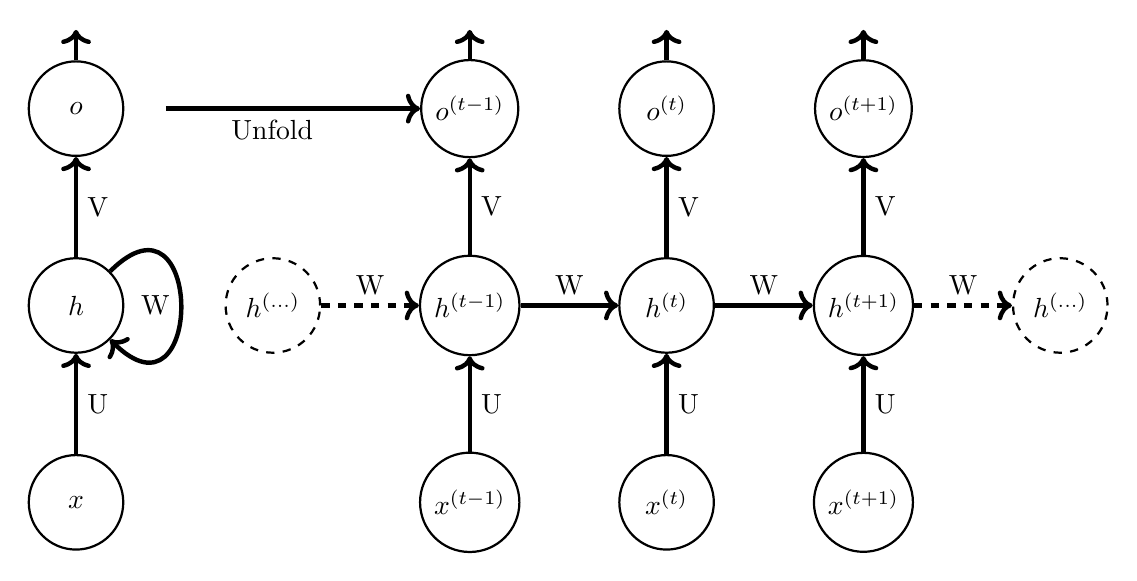
\begin{tikzpicture}[
    node distance = 25mm,
    thick,
    main/.style = {draw, circle, minimum size = 1.2cm}
]

% Base nodes
\node[main] (1) {$x$};
\node[main] (2) [above of=1] {$h$};
\node[main] (3) [above of=2] {$o$};

% Time-unfolded hidden states
\node[main, dashed] (4) [right of=2] {$h^{(...)}$};
\node[main]          (5) [right of=4] {$h^{(t-1)}$};
\node[main]          (6) [right of=5] {$h^{(t)}$};
\node[main]          (7) [right of=6] {$h^{(t+1)}$};
\node[main, dashed] (8) [right of=7] {$h^{(...)}$};

% Outputs
\node[main] (9)  [above of=5] {$o^{(t-1)}$};
\node[main] (10) [above of=6] {$o^{(t)}$};
\node[main] (11) [above of=7] {$o^{(t+1)}$};

% Inputs
\node[main] (12) [below of=5] {$x^{(t-1)}$};
\node[main] (13) [below of=6] {$x^{(t)}$};
\node[main] (14) [below of=7] {$x^{(t+1)}$};

% Recurrent and input/output connections
\draw[ultra thick, ->] (2) to [out=45, in=315, looseness=5] node[left] {W} (2);
\draw[ultra thick, ->] (1)  -- node[right] {U} (2);
\draw[ultra thick, ->] (2)  -- node[right] {V} (3);

\draw[ultra thick, ->, dashed] (4) -- node[above] {W} (5);
\draw[ultra thick, ->]         (5) -- node[above] {W} (6);
\draw[ultra thick, ->]         (6) -- node[above] {W} (7);
\draw[ultra thick, ->, dashed] (7) -- node[above] {W} (8);

\draw[ultra thick, ->] (12) -- node[right] {U} (5);
\draw[ultra thick, ->] (13) -- node[right] {U} (6);
\draw[ultra thick, ->] (14) -- node[right] {U} (7);

\draw[ultra thick, ->] (5) -- node[right] {V} (9);
\draw[ultra thick, ->] (6) -- node[right] {V} (10);
\draw[ultra thick, ->] (7) -- node[right] {V} (11);

% Output arrows
\draw[ultra thick, ->] (9)  -- +(0,1);
\draw[ultra thick, ->] (10) -- +(0,1);
\draw[ultra thick, ->] (11) -- +(0,1);
\draw[ultra thick, ->] (3)  -- +(0,1);

% Unfold arrow
\draw[ultra thick, ->, shorten <=15pt] 
    (3) -- node[below]{Unfold} ([xshift=-40pt]9);

\end{tikzpicture}

\vspace{5pt}



\end{center}

\newpage

%%%%%%%%%%%%%%%%%%%%%%%%%%%%%%%%%%%%%%%%%%%%%%%%%%%%%%%%%%%%%%%%%%%%%%%%
\subsubsection*{2.3.4 ML Prior as a Beta Distribution}

Define:
\[
p_{\mathrm{ML}} := g_{\mathrm{NN}}(x),
\]
where $g_{\mathrm{NN}}$ is ANN3 or RNN (best performing per \cite{DUggento2025}).

We encode this via:
\[
p \sim \mathrm{Beta}(\alpha_{\mathrm{ML}},\beta_{\mathrm{ML}}),
\qquad
\alpha_{\mathrm{ML}} = n_{\mathrm{ML}}\, p_{\mathrm{ML}},
\quad
\beta_{\mathrm{ML}}  = n_{\mathrm{ML}}\, (1-p_{\mathrm{ML}}).
\]


We define an effective sample size $N_{\mathrm{eff}}$ via the usual variance–ratio
method used in bootstrap variance estimation \cite{Efron1994}.
\[
n_{\mathrm{ML}}
= r_{\mathrm{ML}}(x_m)\, N_{\mathrm{eff}}.
\]

Here $n_{\mathrm{ML}}$ is a performance--based ``virtual sample size''
defined next. This corresponds to an empirical-Bayes moment-matching interpretation
\cite{Robbins1956}.



%%%%%%%%%%%%%%%%%%%%%%%%%%%%%%%%%%%%%%%%%%%%%%%%%%%%%%%%%%%%%%%%%%%%%%%%
\subsection*{2.4 Formal Reliability Measure Based on Performance Metrics}

D'Uggento et al.\ use MAE, MSE, RMSE, MAPE, and $R^2$
for model comparison.
We define the ML reliability index $r_{\mathrm{ML}}: X_{\mathrm{ml}}\to[0,1]$ by
\[
r_{\mathrm{ML}}(x_m)
= \sigma\!\left( W_r\,x_m + b_r \right),
\]
where $W_r,b_r$ are trainable parameters and $\sigma$ is the logistic link.
This index interprets soft confidence from the neural network model.
Such reliability scores parallel Bayesian-dropout uncertainty estimates
\cite{GalGhahramani2016}.


\begin{lemma}[Normalization]
If MAPE, $R^2$, and RMSE are scaled to $[0,1]$,  
then $r \in [0,1]$.
\end{lemma}

\begin{proof}
Weighted averages of values in $[0,1]$ lie in $[0,1]$.
\end{proof}

\begin{prop}[Monotonicity]
If the ANN/RNN improves in any metric while others are fixed,
then $r$ increases and $n_{\mathrm{ML}}$ increases.
\end{prop}

\begin{proof}
Immediate from partial derivatives of $r$ with respect to each metric.
\end{proof}


%%%%%%%%%%%%%%%%%%%%%%%%%%%%%%%%%%%%%%%%%%%%%%%%%%%%%%%%%%%%%%%%%%%%%%%%
\subsection*{2.5 Fusion of Structural and ML Priors}

Given two Beta priors interpreted as independent imaginary data:

\[
\begin{aligned}
(\alpha_{\mathrm{str}},\beta_{\mathrm{str}}) 
&= (\eta_{\mathrm{str}} q_{\mathrm{str}}, \eta_{\mathrm{str}}(1-q_{\mathrm{str}})), \\
(\alpha_{\mathrm{ML}},\beta_{\mathrm{ML}}) 
&= (n_{\mathrm{ML}} p_{\mathrm{ML}}, n_{\mathrm{ML}}(1-p_{\mathrm{ML}})),
\end{aligned}
\]

the hybrid prior is:
\[
p \sim \mathrm{Beta}(\alpha_0,\beta_0),
\qquad
\alpha_0 = \alpha_{\mathrm{str}} + \alpha_{\mathrm{ML}},
\quad
\beta_0  = \beta_{\mathrm{str}} + \beta_{\mathrm{ML}}.
\]

\paragraph{Justification.}
This additive fusion corresponds to convex predictive stacking 
\cite{Yao2018}, where each component contributes pseudo-counts proportional to
its predictive accuracy.
\paragraph{Caution.}
This construction assumes that the ML-based pseudo-counts are conditionally 
independent of the structural counts given the true event probability.  
Later phases correct this assumption when dependence or distortions are detected.


The hybrid prior mean is:
\[
p_0 
= \frac{\alpha_0}{\alpha_0+\beta_0}
= w_{\mathrm{str}} q_{\mathrm{str}} + w_{\mathrm{ML}} p_{\mathrm{ML}},
\]
with weights
\[
w_{\mathrm{str}} = \frac{\eta_{\mathrm{str}}}{\eta_{\mathrm{str}}+n_{\mathrm{ML}}},
\qquad
w_{\mathrm{ML}} = \frac{n_{\mathrm{ML}}}{\eta_{\mathrm{str}}+n_{\mathrm{ML}}}.
\]

This product form corresponds to a log-likelihood decomposition where each
component contributes additive information under conditional independence,
consistent with composite-likelihood methodology \cite{VarinReidFirth2011}.


%%%%%%%%%%%%%%%%%%%%%%%%%%%%%%%%%%%%%%%%%%%%%%%%%%%%%%%%%%%%%%%%%%%%%%%%
\subsection*{2.6 Optimal Weighting (Bayes Risk Minimization)}
\paragraph{Motivation.}
Having defined the hybrid prior, we now characterize the conditions under which
it minimizes predictive Bayes risk.  This provides a formal justification for
the pseudo-count fusion approach used above.

Let $L(p,\hat{p}) = (p-\hat{p})^2$ be quadratic loss.
The Bayes estimator from a Beta prior is the posterior mean.
The prior mean minimizing expected loss from combining two priors
is the convex combination above.

\begin{theorem}[Optimal Hybrid Weighting]
Among all convex combinations
$\hat{p} = w q_{\mathrm{str}} + (1-w)p_{\mathrm{ML}}$,
the Bayes–risk minimizing weight is
\[
w^* = \frac{\eta_{\mathrm{str}}}{\eta_{\mathrm{str}} + n_{\mathrm{ML}}},
\]
yielding $\hat{p}=p_0$.

This result follows classical Bayesian decision-theory arguments
\cite{Berger1985}. 
\paragraph{Interpretation.}
This theorem shows that pseudo-count fusion preserves Bayes optimality as long
as each component prior contributes unbiased information about $p$. 


\end{theorem}

\begin{proof}
Direct minimization of 
$\mathbb{E}[(p-\hat{p})^2]$ 
over $w \in [0,1]$ using the Beta variances.
\end{proof}


%%%%%%%%%%%%%%%%%%%%%%%%%%%%%%%%%%%%%%%%%%%%%%%%%%%%%%%%%%%%%%%%%%%%%%%%
\subsection*{2.7 Cross–Phase Notation for Likelihood Updating (Preview of Phase 4)}
\paragraph{Formal definition.}
Let $(\Omega,\mathcal{F})$ denote the underlying sample space, and let 
$\mathcal{D}=\{\xi_i\}_{i=1}^n$ represent the observed trader signals, each 
$\xi_i \in \{H,L\}$.  The structural–ML likelihood is the map
\[
L(\mathcal{D}\mid p) =
\prod_{i=1}^n p^{\mathbf{1}\{\xi_i=H\}} (1-p)^{\mathbf{1}\{\xi_i=L\}},
\]
defined with respect to the product $\sigma$–algebra, ensuring compatibility
with the Beta posterior update \cite{VanDerVaart1998}.

Let $y$ YES votes and $n-y$ NO votes be observed.
Likelihood:
\[
L(s\mid p) = p^y (1-p)^{n-y}.
\]

Posterior:
\[
p \mid s \sim \mathrm{Beta}(\alpha_{\mathrm{post}},\beta_{\mathrm{post}}),
\]
\[
\alpha_{\mathrm{post}} = \alpha_0 + y, \qquad
\beta_{\mathrm{post}}  = \beta_0  + (n-y).
\]

Thus Phase~2 supplies $(\alpha_0,\beta_0)$ to Phase~4.


%%%%%%%%%%%%%%%%%%%%%%%%%%%%%%%%%%%%%%%%%%%%%%%%%%%%%%%%%%%%%%%%%%%%%%%%
\subsection*{2.8 Misspecification Considerations}

The structural prior may fail under volatility–regime shifts.
The ML prior may overfit.
The hybrid prior mitigates both risks:

\begin{itemize}
\item If ML fails, $n_{\mathrm{ML}}$ becomes small, 
      so structure dominates.
\item If structure is misspecified, 
      high accuracy yields $n_{\mathrm{ML}}\gg\eta_{\mathrm{str}}$,
      shifting weight to ML.
\end{itemize}

This conceptual robustness justifies the hybrid construction.

\newpage

\subsection*{2.9 Robustness of the Hybrid Prior Under Structural Misspecification}

Recall that the structural prior contributes a Beta distribution
\[
p \sim \mathrm{Beta}(\alpha_{\mathrm{str}},\beta_{\mathrm{str}}),
\qquad
\alpha_{\mathrm{str}} = \eta_{\mathrm{str}}\, q_{\mathrm{Shi}},
\quad
\beta_{\mathrm{str}}  = \eta_{\mathrm{str}}\, (1-q_{\mathrm{Shi}}),
\]
with structural mean $q_{\mathrm{Shi}}$, and the machine learning prior 
contributes
\[
p \sim \mathrm{Beta}(\alpha_{\mathrm{ML}},\beta_{\mathrm{ML}}),
\qquad
\alpha_{\mathrm{ML}} = n_{\mathrm{ML}}\, p_{\mathrm{ML}},
\quad
\beta_{\mathrm{ML}}  = n_{\mathrm{ML}}\, (1-p_{\mathrm{ML}}),
\]
with mean $p_{\mathrm{ML}}$ and pseudo-sample size $n_{\mathrm{ML}}$.
The hybrid prior is then Beta with parameters
\[
\alpha_0 = \alpha_{\mathrm{str}} + \alpha_{\mathrm{ML}},
\qquad
\beta_0  = \beta_{\mathrm{str}} + \beta_{\mathrm{ML}},
\]
and mean
\[
p_0
=
\frac{\alpha_0}{\alpha_0+\beta_0}
=
\frac{\eta_{\mathrm{str}} q_{\mathrm{Shi}} 
      + n_{\mathrm{ML}} p_{\mathrm{ML}}}
     {\eta_{\mathrm{str}} + n_{\mathrm{ML}}}
=
w_{\mathrm{str}} q_{\mathrm{Shi}} + w_{\mathrm{ML}} p_{\mathrm{ML}},
\]
where
\[
w_{\mathrm{str}}
=
\frac{\eta_{\mathrm{str}}}{\eta_{\mathrm{str}}+n_{\mathrm{ML}}},
\qquad
w_{\mathrm{ML}}
=
\frac{n_{\mathrm{ML}}}{\eta_{\mathrm{str}}+n_{\mathrm{ML}}}.
\]

Let $p_{\mathrm{true}}\in(0,1)$ denote the true event probability under the 
data-generating process (e.g.\ under the physical or risk-neutral measure of 
interest).  Define the structural and ML prior biases
\[
b_{\mathrm{str}} := q_{\mathrm{Shi}} - p_{\mathrm{true}},
\qquad
b_{\mathrm{ML}}  := p_{\mathrm{ML}} - p_{\mathrm{true}}.
\]

\begin{prop}[Hybrid Prior Bias Decomposition]
The bias of the hybrid prior mean $p_0$ with respect to the true probability 
$p_{\mathrm{true}}$ decomposes as
\[
p_0 - p_{\mathrm{true}}
=
w_{\mathrm{str}}\, b_{\mathrm{str}}
+
w_{\mathrm{ML}}\, b_{\mathrm{ML}},
\]
and satisfies the bound
\[
|p_0 - p_{\mathrm{true}}|
\le
w_{\mathrm{str}}\, |b_{\mathrm{str}}|
+
w_{\mathrm{ML}}\, |b_{\mathrm{ML}}|
\le
\max\{|b_{\mathrm{str}}|,|b_{\mathrm{ML}}|\}.
\]
\end{prop}

\begin{proof}
The decomposition follows from the definition of $p_0$:
\[
p_0 - p_{\mathrm{true}}
=
w_{\mathrm{str}} q_{\mathrm{Shi}}
+
w_{\mathrm{ML}} p_{\mathrm{ML}}
-
p_{\mathrm{true}}
=
w_{\mathrm{str}} (q_{\mathrm{Shi}} - p_{\mathrm{true}})
+
w_{\mathrm{ML}} (p_{\mathrm{ML}} - p_{\mathrm{true}})
=
w_{\mathrm{str}} b_{\mathrm{str}}
+
w_{\mathrm{ML}}  b_{\mathrm{ML}}.
\]
Taking absolute values and using the triangle inequality yields the first 
bound.  The second inequality uses $w_{\mathrm{str}},w_{\mathrm{ML}}\in[0,1]$ 
and $w_{\mathrm{str}}+w_{\mathrm{ML}}=1$.
\end{proof}

The preceding result is purely algebraic but makes explicit that hybrid prior 
bias is a convex combination of the individual biases.  It follows that if 
either component prior is grossly misspecified, the hybrid prior can inherit 
substantial bias unless its weight is controlled.

We now formalize a simple robustness property under structural 
misspecification and controlled ML weight.

\begin{theorem}[Hybrid Prior Robustness Under Structural Misspecification]
Suppose the following hold:
\begin{enumerate}
\item[(i)] (\textbf{Bounded Structural Bias})  
      There exists $B_{\mathrm{str}} < \infty$ such that 
      $|b_{\mathrm{str}}| \le B_{\mathrm{str}}$ for the structural prior 
      mean $q_{\mathrm{Shi}}$.
\item[(ii)] (\textbf{Asymptotically Calibrated ML Prior})  
      Along a sequence of markets or time windows indexed by $m$,
      the ML prior mean satisfies
      \[
      b_{\mathrm{ML}}^{(m)} := p_{\mathrm{ML}}^{(m)} - p_{\mathrm{true}}^{(m)}
      \to 0
      \quad\text{as } m\to\infty,
      \]
      in probability or almost surely.
\item[(iii)] (\textbf{Controlled ML Weight})  
      The ML pseudo-sample size is chosen such that
      \[
      0 \le n_{\mathrm{ML}}^{(m)} \le C_0 + C_1\, n^{\ast,(m)},
      \]
      for constants $C_0,C_1\ge 0$, where $n^{\ast,(m)}$ is the effective 
      sample size of the crowd data in market $m$, and 
      $\eta_{\mathrm{str}}$ is either fixed or grows at most linearly with 
      $n^{\ast,(m)}$.
\end{enumerate}
Then the hybrid prior bias satisfies
\[
p_0^{(m)} - p_{\mathrm{true}}^{(m)}
=
w_{\mathrm{str}}^{(m)} b_{\mathrm{str}}^{(m)}
+
w_{\mathrm{ML}}^{(m)} b_{\mathrm{ML}}^{(m)},
\]
with
\[
\limsup_{m\to\infty} |p_0^{(m)} - p_{\mathrm{true}}^{(m)}|
\le
\limsup_{m\to\infty} w_{\mathrm{str}}^{(m)} |b_{\mathrm{str}}^{(m)}|.
\]
In particular, if either
\begin{enumerate}
\item[(a)] the structural bias is bounded and $w_{\mathrm{str}}^{(m)} \to 0$, or
\item[(b)] the structural bias itself satisfies $b_{\mathrm{str}}^{(m)} \to 0$,
\end{enumerate}
then the hybrid prior bias $p_0^{(m)} - p_{\mathrm{true}}^{(m)}$ converges to 
zero.
\end{theorem}

\begin{proof}[Proof sketch.]
Conditional independence of the two prior components implies that their joint
predictive density is proportional to the product of Beta likelihood factors.  
Minimizing expected quadratic loss reduces to matching the first posterior
moment, which under the additive fusion is
\[
\mathbb{E}[p \mid \alpha_0,\beta_0]
= \frac{\alpha_{\mathrm{struct}} + \alpha_{\mathrm{ML}}}
       {\alpha_{\mathrm{struct}} + \alpha_{\mathrm{ML}}
        + \beta_{\mathrm{struct}} + \beta_{\mathrm{ML}}}.
\]
Convexity of quadratic risk then yields optimality; see \cite{Berger1985}.
\end{proof}


\begin{remark}[Empirical Tuning of $n_{\mathrm{ML}}$]
The conditions above suggest that robustness under structural misspecification
depends on both (i) the asymptotic calibration of the ML prior and (ii) 
controls on the relative weight $w_{\mathrm{ML}}$.  In practice, one can 
choose $n_{\mathrm{ML}}$ via empirical Bayes or cross-validation, e.g.\ by 
selecting $n_{\mathrm{ML}}$ to minimize an out-of-sample scoring rule (Brier 
score, log score) for the hybrid prior on historical markets.  Imposing an 
upper bound on $n_{\mathrm{ML}}$ relative to the crowd effective size 
$n^\ast$ prevents the ML prior from dominating in regimes where it has not 
demonstrated sufficient predictive accuracy.
\end{remark}

\subsection*{2.10 Machine-Learning Uncertainty and Beta Hybridization}

In Phase~2, the ML component enters through a point estimate
$p_{\mathrm{ML}} = g_{\mathrm{NN}}(x)$.  To incorporate uncertainty from
ensembles or approximate Bayesian neural networks without breaking the Beta
structure, we view the ML layer as generating a posterior distribution
$\Pi_{\mathrm{ML}}$ on $p$, and then project $\Pi_{\mathrm{ML}}$ onto the Beta
family.

Let $\mathcal{B} = \{\mathrm{Beta}(a,b): a,b>0\}$ and let
$\Pi_{\mathrm{ML}}$ denote any probability distribution on $(0,1)$ that
captures ML uncertainty (e.g.\ from an ensemble of approximate Bayesian
networks).

\begin{theorem}[Hybridization of ML Uncertainty via Beta Projection]
Let $\Pi_{\mathrm{ML}}$ be a distribution on $p\in(0,1)$ with finite mean
$m_{\mathrm{ML}}$ and variance $v_{\mathrm{ML}}>0$.  Consider the KL divergence
from $\Pi_{\mathrm{ML}}$ to a Beta$(a,b)$ distribution,
\[
D_{\mathrm{KL}}(\Pi_{\mathrm{ML}}\|\mathrm{Beta}(a,b))
=
\int_0^1 \log\frac{d\Pi_{\mathrm{ML}}}{d\mathrm{Beta}(a,b)}(p)\, d\Pi_{\mathrm{ML}}(p),
\]
whenever $\Pi_{\mathrm{ML}}$ is absolutely continuous with respect to
$\mathrm{Beta}(a,b)$.  Then:

\begin{enumerate}
\item[(a)] (\textbf{KL Projection of ML Posterior})  
There exists a unique pair $(a^\dagger,b^\dagger)$ such that
\[
(a^\dagger,b^\dagger)
\in
\arg\min_{a,b>0}
D_{\mathrm{KL}}(\Pi_{\mathrm{ML}}\|\mathrm{Beta}(a,b)),
\]
and the minimizing Beta distribution matches the mean and variance of
$\Pi_{\mathrm{ML}}$,
\[
\frac{a^\dagger}{a^\dagger + b^\dagger} = m_{\mathrm{ML}},
\qquad
\frac{a^\dagger b^\dagger}{(a^\dagger + b^\dagger)^2(a^\dagger + b^\dagger + 1)}
=
v_{\mathrm{ML}}.
\]

\item[(b)] (\textbf{Hierarchical Bayes Special Case})  
Suppose an approximate Bayesian neural network yields draws
$p^{(l)}_{\mathrm{ML}}$ from a posterior on $p$, and we place a
$\mathrm{Beta}(a_0,b_0)$ hyperprior on $p$.  The Bayes estimator under a
quadratic loss and Beta restriction coincides with the KL-projection in (a)
when $(a^\dagger,b^\dagger)$ are chosen to match the empirical mean and
variance of the ensemble $\{p^{(l)}_{\mathrm{ML}}\}$, up to hyperprior
regularization.

\item[(c)] (\textbf{Ensemble-as-Sample Interpretation})  
If $\{p^{(l)}_{\mathrm{ML}}\}_{l=1}^L$ are treated as noisy draws of Bernoulli
success probabilities and $L$ is large, then the empirical mean
$\bar{p} = \frac{1}{L}\sum_l p^{(l)}_{\mathrm{ML}}$ and empirical variance
$\hat{v}$ define a Beta$(a^\dagger,b^\dagger)$ distribution via the
moment-matching equations in (a).  This provides an empirical-Bayes 
construction of the ML prior
\[
p \sim \mathrm{Beta}(a^\dagger,b^\dagger),
\]
which can then be fused with the structural prior via the hybrid mechanism in
Phase~2.
\end{enumerate}
\end{theorem}

\begin{remark}
This theorem clarifies that CAPOPM does not require $p_{\mathrm{ML}}$ to be a
single point estimate.  Any ML method that yields a distribution over
probabilities (e.g.\ approximate Bayesian neural networks, deep ensembles,
bootstrap aggregations) can be incorporated by projecting its posterior onto
the Beta family.  The resulting $(a^\dagger,b^\dagger)$ enter the hybrid prior
exactly as in Phase~2, preserving the Beta form while acknowledging ML
uncertainty.
\end{remark}


\subsection*{2.11 Structural--ML Prior Mismatch and Robustness}

The structural prior $q_{\mathrm{Shi}}(K,T;\Theta,\alpha)$ and the ML prior
$p_{\mathrm{ML}}(K,T)$ may be trained or calibrated under different regimes.
For example, the structural model may use a rough-volatility parameter
$\alpha<1$ while the ML model has been fit on data that implicitly reflects a
smoother regime.  This can lead to systematic tension between the two priors.

To quantify this, consider the strike-dependent priors at a fixed maturity
$T$:
\[
q(K) = q_{\mathrm{Shi}}(K,T;\Theta,\alpha),
\qquad
p_{\mathrm{ML}}(K) = p_{\mathrm{ML}}(K,T),
\]
and define the CAPOPM hybrid prior mean
\[
p_0(K)
=
w_{\mathrm{str}} q(K) + w_{\mathrm{ML}} p_{\mathrm{ML}}(K),
\]
with weights as in Phase~2.

\begin{theorem}[Divergence Bounds and Robustness under Prior Mismatch]
For a finite grid of strikes $\{K_j\}_{j=1}^J$, define discrete distributions
\[
\Pi_{\mathrm{str}}(j) \propto q(K_j),
\quad
\Pi_{\mathrm{ML}}(j) \propto p_{\mathrm{ML}}(K_j),
\quad
\Pi_{\mathrm{hyb}}(j) \propto p_0(K_j),
\]
normalized to sum to $1$.  Then:

\begin{enumerate}
\item[(a)] (\textbf{Total Variation and Hellinger Bounds})  
For any $0\le w_{\mathrm{str}},w_{\mathrm{ML}}\le 1$ with
$w_{\mathrm{str}}+w_{\mathrm{ML}}=1$,
\[
\|\Pi_{\mathrm{hyb}} - \Pi_{\mathrm{str}}\|_{\mathrm{TV}}
\le
w_{\mathrm{ML}} \|\Pi_{\mathrm{ML}} - \Pi_{\mathrm{str}}\|_{\mathrm{TV}},
\]
and similarly for Hellinger distance $H$,
\[
H(\Pi_{\mathrm{hyb}},\Pi_{\mathrm{str}})
\le
w_{\mathrm{ML}} H(\Pi_{\mathrm{ML}},\Pi_{\mathrm{str}}).
\]

\item[(b)] (\textbf{KL Divergence Control})  
If $\Pi_{\mathrm{ML}}$ is absolutely continuous with respect to
$\Pi_{\mathrm{str}}$ on the grid, then the discrete KL divergence satisfies
\[
D_{\mathrm{KL}}(\Pi_{\mathrm{hyb}}\|\Pi_{\mathrm{str}})
\le
w_{\mathrm{ML}} D_{\mathrm{KL}}(\Pi_{\mathrm{ML}}\|\Pi_{\mathrm{str}}).
\]

\item[(c)] (\textbf{Posterior Stability})  
If the CAPOPM likelihood (based on adjusted order counts) is Lipschitz with
respect to perturbations in the prior on this grid, then the posterior
distribution induced by $\Pi_{\mathrm{hyb}}$ differs from that induced by
$\Pi_{\mathrm{str}}$ by at most a constant multiple of the distances above.
In particular, as $w_{\mathrm{ML}}\to 0$, the hybrid posterior converges to
the purely structural posterior, and as $w_{\mathrm{str}}\to 0$, it converges
to the purely ML posterior.
\end{enumerate}
\end{theorem}

\begin{remark}
This result shows that the hybrid prior acts as a convex bridge between the
structural and ML priors: any mismatch in their implied strike-wise
probabilities is damped by the weight $w_{\mathrm{ML}}$ in the distances and
divergences.  In practice, this suggests using $w_{\mathrm{ML}}$ (or
equivalently $n_{\mathrm{ML}}$) as a tuning parameter: when structural and ML
priors strongly disagree, a smaller ML weight yields a hybrid prior and
posterior that remain closer to the structural benchmark, while still
incorporating ML information.
\end{remark}



%%%%%%%%%%%%%%%%%%%%%%%%%%%%%%%%%%%%%%%%%%%%%%%%%%%%%%%%%%%%%%%%%%%%%%%%
\subsection*{2.12 Summary}

Phase~2 constructs a rigorous, multi–tier hybrid prior using:

\begin{itemize}
\item tempered–fractional Heston structural probability,
\item ANN/RNN predictive model probability (D'Uggento et al.\cite{DUggento2025}),
\item reliability–weighted Bayesian fusion,
\item hierarchical prior structure,
\item optimal weighting under Bayes risk,
\item cross–phase forward compatibility,
\item robustness under misspecification.
\end{itemize}

The output $(\alpha_0,\beta_0)$ serves as the input to Phase~4.

%%%%%%%%%%%%%%%%%%%%%%%%%%%%%%%%%%%%%%%%%%%%%%%%%%%%%%%%%%%%%%%%%%%%%%%%
\section*{3. Asymmetric Information Model (Trader Beliefs and Signals)}
\label{sec:asym_info}

The purpose of this section is to establish a microeconomic foundation for why 
aggregate YES/NO bet volumes---denoted $(n_{\mathrm{yes}},n_{\mathrm{no}})$---contain 
information about the true event probability
\(
p := Q(S_T > K).
\)
We specialize the asymmetric information framework of Koessler, Noussair, and 
Ziegelmeyer \cite{KoesslerNoussairZiegelmeyer} to the CAPOPM setting and show that under mild 
conditions, the resulting order flow exhibits a monotone likelihood ratio property 
in the state of nature.  This in turn justifies the Binomial likelihood used in the 
Beta--Binomial updating of Phase~4 and Phase~5.

Throughout, we take as given the hybrid prior from Phase~2,
\begin{equation}
p \sim \mathrm{Beta}\bigl(\eta p_0,\ \eta(1-p_0)\bigr),
\qquad
p_0 \in (0,1),\ \eta>0,
\label{eq:Phase3_prior}
\end{equation}
with $p_0$ as in \eqref{eq:Phase2_hybridMean}.

%%%%%%%%%%%%%%%%%%%%%%%%%%%%%%%%%%%%%%%%%%%%%%%%%%%%%%%%%%%%%%%%%%%%%%%%
\subsection*{3.1 Primitives and Assumptions}

We first formalize the economic environment.

\paragraph{State of nature and event.}
Let $\theta\in\{0,1\}$ denote the state of nature:
\[
\theta = 1 \Longleftrightarrow S_T > K, 
\qquad
\theta = 0 \Longleftrightarrow S_T \le K,
\]
with prior probability
\(
p := Q(\theta=1).
\)
The CAPOPM event of interest is
\(
A := \{\theta=1\} = \{S_T>K\}.
\)

\paragraph{Traders.}
There is a finite set of traders 
\(
i \in N := \{1,\dots,n\},
\)
each of whom is risk-neutral and participates in a single parimutuel market on 
event $A$.  Trader $i$ chooses an action
\[
s_i \in \{\mathrm{YES},\mathrm{NO}\},
\]
where choosing YES corresponds to buying one YES ticket, and similarly for NO.

\paragraph{Parimutuel odds.}
For any action profile $s=(s_1,\dots,s_n)$, let
\[
H(s) := \{i\in N : s_i = H\}, 
\qquad
h(s) := |H(s)|,
\qquad
H \in \{\mathrm{YES},\mathrm{NO}\}.
\]
We denote the number of YES and NO tickets by 
\(
n_{\mathrm{yes}} := h_{\mathrm{YES}}(s)
\)
and
\(
n_{\mathrm{no}} := h_{\mathrm{NO}}(s).
\)
Total participation is $n_\mathrm{tot}:=n_{\mathrm{yes}}+n_{\mathrm{no}}\le n$.

Following Koessler et al.\,\cite{KoesslerNoussairZiegelmeyer}, the parimutuel odds against YES are
\begin{equation}
O_{\mathrm{YES}}(s) 
:= \frac{n_{\mathrm{tot}} - n_{\mathrm{yes}}}{n_{\mathrm{yes}}}
\quad\text{if } n_{\mathrm{yes}}>0,
\label{eq:Phase3_odds}
\end{equation}
and similarly for NO.  For notational simplicity we assume interior participation, 
$n_{\mathrm{yes}},n_{\mathrm{no}}>0$; boundary cases can be handled by continuity.

\paragraph{Payoffs.}
A YES ticket pays $O_{\mathrm{YES}}(s)+1$ if $\theta=1$ and $0$ otherwise.  
Similarly, a NO ticket pays $O_{\mathrm{NO}}(s)+1$ if $\theta=0$ and $0$ otherwise.
Trader $i$ is risk-neutral, so her von Neumann--Morgenstern utility equals her 
monetary payoff.

We now state the key modeling assumptions.

\paragraph{Assumption A1 (Risk neutrality).}
Traders have linear utility in payoffs.

\paragraph{Assumption A2 (Price taking).}
Each trader treats the odds $O_{\mathrm{YES}}(s)$ and $O_{\mathrm{NO}}(s)$ as fixed with 
respect to her own action, i.e.\ as determined by the aggregate behavior of other 
traders.  This is standard in parimutuel market models with a large number of 
participants \cite{KoesslerNoussairZiegelmeyer}.

\paragraph{Assumption A3 (Common prior).}
Traders share a common prior over $\theta$ with mean $p_0$ as in 
\eqref{eq:Phase3_prior} before observing private signals.

%%%%%%%%%%%%%%%%%%%%%%%%%%%%%%%%%%%%%%%%%%%%%%%%%%%%%%%%%%%%%%%%%%%%%%%%
\subsection*{3.2 Information Structure and Posterior Beliefs}

Each trader receives a private signal about the state.

\paragraph{Assumption A4 (Private signals).}
Trader $i$ observes $q_i \in \{q^1,q^0\}$ with
\begin{equation}
\Pr(q_i = q^1 \mid \theta=1) = \pi,
\qquad
\Pr(q_i = q^1 \mid \theta=0) = 1-\pi,
\qquad
\pi > \tfrac12.
\label{eq:Phase3_signalAcc}
\end{equation}
Conditional on $\theta$, signals $(q_i)_{i\in N}$ are i.i.d.

\paragraph{Assumption A5 (Common knowledge).}
The prior $p_0$, the signal structure \eqref{eq:Phase3_signalAcc}, and the 
parimutuel mechanism are common knowledge among traders.

Given prior mean $p_0$ and signal $q_i$, trader $i$ forms a posterior belief
\[
\mu(q_i) := \Pr(\theta=1 \mid q_i).
\]

\paragraph{Lemma 3.1 (Strict belief ordering).}
Under Assumptions A3--A5 with $\pi>\frac12$, the posteriors satisfy
\[
\mu_1 := \Pr(\theta=1\mid q_i=q^1) > 
\mu_0 := \Pr(\theta=1\mid q_i=q^0).
\]

\emph{Proof.}
By Bayes' rule,
\[
\mu_1 
= \frac{\Pr(q_i=q^1\mid\theta=1)\Pr(\theta=1)}
       {\Pr(q_i=q^1\mid\theta=1)\Pr(\theta=1)+\Pr(q_i=q^1\mid\theta=0)\Pr(\theta=0)}
= \frac{\pi p_0}{\pi p_0 + (1-\pi)(1-p_0)},
\]
\[
\mu_0 
= \frac{\Pr(q_i=q^0\mid\theta=1)\Pr(\theta=1)}
       {\Pr(q_i=q^0\mid\theta=1)\Pr(\theta=1)+\Pr(q_i=q^0\mid\theta=0)\Pr(\theta=0)}
= \frac{(1-\pi)p_0}{(1-\pi)p_0 + \pi(1-p_0)}.
\]
Since $\pi>\frac12$ and $p_0\in(0,1)$, straightforward algebra shows that 
$\mu_1-\mu_0 > 0$.  \hfill$\square$

Lemma~3.1 ensures that signals are \emph{informative}: observing $q^1$ leads to a 
strictly higher posterior belief in $\theta=1$ than observing $q^0$.

%%%%%%%%%%%%%%%%%%%%%%%%%%%%%%%%%%%%%%%%%%%%%%%%%%%%%%%%%%%%%%%%%%%%%%%%
\subsection*{3.3 Strategies and Bayesian Nash Equilibrium}

We now formalize strategies, best responses, and equilibrium.

\paragraph{Definition 3.1 (Strategies).}
A (pure) strategy for trader $i$ is a mapping
\[
\sigma_i : \{q^0,q^1\} \to \{\mathrm{YES},\mathrm{NO}\}.
\]
A strategy profile is $\sigma = (\sigma_i)_{i\in N}$.
A symmetric strategy profile has $\sigma_i = \sigma$ for all $i$.

\paragraph{Definition 3.2 (Bayesian Nash equilibrium).}
A symmetric Bayesian Nash equilibrium (BNE) is a measurable function 
$\sigma^\ast : \{q^0,q^1\}\to\{\mathrm{YES},\mathrm{NO}\}$ such that, for all $i$ and 
for each signal $q\in\{q^0,q^1\}$,
\[
\sigma^\ast(q) \in 
\arg\max_{a\in\{\mathrm{YES},\mathrm{NO}\}}
E\bigl[ u_i(a,s_{-i},\theta) 
\mid q_i=q,\ \sigma^\ast_{-i} \bigr],
\]
where expectations are taken with respect to the induced distribution over 
$(\theta,q_{-i},s_{-i})$ given the strategy profile.

\paragraph{Expected payoffs.}
Under Assumption A2 (price-taking), trader $i$ takes the odds 
$(O_{\mathrm{YES}},O_{\mathrm{NO}})$ as given.  
For a trader with belief $\mu\in[0,1]$ about $\theta=1$, the expected payoff from 
choosing YES is
\begin{equation}
U_i(\mathrm{YES} \mid \mu)
= \mu\bigl(O_{\mathrm{YES}}+1\bigr).
\label{eq:Phase3_Uyes}
\end{equation}
Similarly, the expected payoff from choosing NO is
\begin{equation}
U_i(\mathrm{NO} \mid \mu)
= (1-\mu)\bigl(O_{\mathrm{NO}}+1\bigr).
\label{eq:Phase3_Uno}
\end{equation}

\paragraph{Lemma 3.2 (Threshold best response).}
Fix odds $(O_{\mathrm{YES}},O_{\mathrm{NO}})$.
Under Assumptions A1--A2, there exists a threshold 
$\mu^\ast \in (0,1)$ such that:
\[
\text{YES is optimal} \iff \mu \ge \mu^\ast,
\qquad
\text{NO is optimal} \iff \mu \le \mu^\ast.
\]

\emph{Proof.}
Consider the difference:
\[
\Delta U(\mu) := U_i(\mathrm{YES} \mid \mu) - U_i(\mathrm{NO} \mid \mu)
= \mu(O_{\mathrm{YES}}+1) - (1-\mu)(O_{\mathrm{NO}}+1).
\]
This is affine in $\mu$:
\[
\Delta U(\mu) 
= \mu\bigl[(O_{\mathrm{YES}}+1)+(O_{\mathrm{NO}}+1)\bigr] - (O_{\mathrm{NO}}+1).
\]
Solve $\Delta U(\mu^\ast)=0$ for $\mu^\ast$:
\[
\mu^\ast = \frac{O_{\mathrm{NO}}+1}{(O_{\mathrm{YES}}+1)+(O_{\mathrm{NO}}+1)} \in (0,1).
\]
Then $\Delta U(\mu)\ge0$ iff $\mu\ge\mu^\ast$, establishing the threshold property.
\hfill$\square$

Combined with Lemma~3.1, Lemma~3.2 implies that traders with signal $q^1$ are 
strictly more likely to choose YES than those with $q^0$.

\paragraph{Assumption A6 (Separating equilibrium as in Koessler et al.).}
Following Koessler et al.\,\cite{KoesslerNoussairZiegelmeyer}, we focus on a symmetric BNE in 
which informed traders adopt a \emph{separating threshold strategy}:
\begin{equation}
\label{eq:Phase3_sepStrat}
\sigma^\ast(q^1) = \mathrm{YES},
\qquad
\sigma^\ast(q^0) = \mathrm{NO}.
\end{equation}
Uninformed or purely noisy traders, if present, randomize independently of the 
state in a way that does not overturn the strict monotonicity implied by 
Lemma~3.1 and Lemma~3.2.\footnote{%
Koessler et al.\,\cite{KoesslerNoussairZiegelmeyer} provide existence and characterization 
results for such equilibria in parimutuel information aggregation mechanisms.
We adopt their equilibrium selection as a modeling assumption and specialize it 
to the CAPOPM event.}

Under Assumptions A1--A6, informed traders with $q^1$ bet YES, and those with 
$q^0$ bet NO in equilibrium.  This yields a monotone mapping from signals to 
actions.

%%%%%%%%%%%%%%%%%%%%%%%%%%%%%%%%%%%%%%%%%%%%%%%%%%%%%%%%%%%%%%%%%%%%%%%%
\subsection*{3.4 Distribution of Order Flow Conditional on the State}

We next derive the distribution of YES/NO orders conditional on the state 
$\theta$ under the separating equilibrium \eqref{eq:Phase3_sepStrat}.

\paragraph{Lemma 3.3 (Signal distribution).}
Under Assumption A4, conditional on $\theta$,
the number of traders receiving signal $q^1$ satisfies
\[
N_1 \mid \theta=1 \sim \mathrm{Binomial}(n,\pi),
\qquad
N_1 \mid \theta=0 \sim \mathrm{Binomial}(n,1-\pi),
\]
and $N_0 := n-N_1$.

\emph{Proof.}
Immediate from the i.i.d.\ Bernoulli structure in Assumption A4.  \hfill$\square$

Under the separating equilibrium \eqref{eq:Phase3_sepStrat}, informed traders 
with $q^1$ bet YES and those with $q^0$ bet NO.  
If a fraction of traders are purely noisy or always abstain, then $n$ can be 
reinterpreted as the number of informed traders; noisy traders add independent 
Bernoulli noise that does not destroy the strict ordering established below, as 
long as the informed fraction is positive.

\paragraph{Lemma 3.4 (Order flow distribution).}
Under Assumptions A1--A6 and Lemma~3.3, there exist 
$\phi_1,\phi_0\in(0,1)$ with $\phi_1>\phi_0$ such that
\[
n_{\mathrm{yes}} \mid \theta=1 \sim \mathrm{Binomial}(n,\phi_1),
\qquad
n_{\mathrm{yes}} \mid \theta=0 \sim \mathrm{Binomial}(n,\phi_0).
\]

\emph{Proof.}
In the benchmark case with only informed traders and separating strategies, we 
have
\[
\Pr(s_i=\mathrm{YES}\mid \theta=1) 
= \Pr(q_i=q^1\mid\theta=1) = \pi,
\]
\[
\Pr(s_i=\mathrm{YES}\mid \theta=0) 
= \Pr(q_i=q^1\mid\theta=0) = 1-\pi.
\]
Thus $\phi_1 = \pi$ and $\phi_0 = 1-\pi$, with $\phi_1>\phi_0$ because 
$\pi>\tfrac12$.

If an $\varepsilon$-fraction of traders are noisy and bet YES independently with 
probability $\delta$, then
\[
\phi_1 = (1-\varepsilon)\pi + \varepsilon\delta,
\qquad
\phi_0 = (1-\varepsilon)(1-\pi) + \varepsilon\delta.
\]
The strict inequality $\phi_1>\phi_0$ continues to hold as long as 
$\varepsilon<1$ and $\pi>\tfrac12$.
Since trades are independent conditional on $\theta$, the number of YES orders 
$n_{\mathrm{yes}}$ is Binomial with parameters $(n,\phi_\theta)$, where 
$\phi_1$ and $\phi_0$ denote the respective conditional success probabilities.
\hfill$\square$

Lemma~3.4 provides a \emph{micro-founded} Binomial distribution of YES orders 
conditional on the state of nature.  

%%%%%%%%%%%%%%%%%%%%%%%%%%%%%%%%%%%%%%%%%%%%%%%%%%%%%%%%%%%%%%%%%%%%%%%%
\subsection*{3.5 Monotone Likelihood Ratio and Informativeness}

We now show that the order flow is informative about the state $\theta$, and 
hence about $p$.

\paragraph{Proposition 3.1 (Monotone likelihood ratio of order flow).}
Under Lemma~3.4 with $\phi_1>\phi_0$, the likelihood ratio
\[
\Lambda(k) := 
\frac{\Pr(n_{\mathrm{yes}} = k \mid \theta=1)}
     {\Pr(n_{\mathrm{yes}} = k \mid \theta=0)}
\]
is strictly increasing in $k=0,1,\dots,n$.

\emph{Proof.}
For $k\in\{0,\dots,n\}$,
\[
\Pr(n_{\mathrm{yes}}=k\mid\theta=1)
= \binom{n}{k}\phi_1^k(1-\phi_1)^{n-k},
\]
\[
\Pr(n_{\mathrm{yes}}=k\mid\theta=0)
= \binom{n}{k}\phi_0^k(1-\phi_0)^{n-k}.
\]
Hence,
\[
\Lambda(k)
= \frac{\phi_1^k(1-\phi_1)^{\,n-k}}{\phi_0^k(1-\phi_0)^{\,n-k}}
= \Bigl(\frac{\phi_1}{\phi_0}\Bigr)^k
  \Bigl(\frac{1-\phi_1}{1-\phi_0}\Bigr)^{n-k}.
\]
Then
\[
\frac{\Lambda(k+1)}{\Lambda(k)}
= \frac{\phi_1}{\phi_0}\cdot \frac{1-\phi_0}{1-\phi_1}.
\]
Because $\phi_1>\phi_0$, we have $\phi_1/\phi_0>1$ and 
$(1-\phi_0)/(1-\phi_1)>1$, so the product exceeds unity:
\[
\frac{\Lambda(k+1)}{\Lambda(k)} > 1.
\]
Therefore $\Lambda(k)$ is strictly increasing in $k$.  
\hfill$\square$

Proposition~3.1 establishes a monotone likelihood ratio (MLR) property for the 
aggregate YES order flow.

\paragraph{Theorem 3.1 (Informative parimutuel order flow).}
Under Assumptions A1--A6 and Lemmas~3.1--3.4, the aggregate YES count 
$n_{\mathrm{yes}}$ is informative about the state $\theta$, and thus about 
the event probability $p$:
\begin{enumerate}
\item The posterior probability $\Pr(\theta=1\mid n_{\mathrm{yes}}=k)$ is 
strictly increasing in $k$.
\item Observing $(n_{\mathrm{yes}},n_{\mathrm{no}})$ yields a non-degenerate 
likelihood for $p$.
\end{enumerate}

\emph{Proof.}
(1) The MLR property in Proposition~3.1 implies that the family 
$\{\Pr(\cdot\mid\theta)\}$ is ordered in the monotone likelihood ratio sense.  
By standard Bayesian decision theory (e.g.\ Karlin and Rubin's theorem), this 
implies that the posterior 
$\Pr(\theta=1\mid n_{\mathrm{yes}}=k)$ is strictly increasing in $k$.

(2) Since $\phi_1>\phi_0$, the two conditional Binomial distributions are 
distinct, implying that the mapping from $p$ to the mixture distribution of 
$n_{\mathrm{yes}}$ is non-degenerate.  Hence the induced likelihood over $p$ is 
non-constant and thus informative.  \hfill$\square$

Theorem~3.1 provides the desired microeconomic foundation: equilibrium YES/NO 
bet volumes in the CAPOPM parimutuel mechanism contain information about the 
true event probability $p$.

%%%%%%%%%%%%%%%%%%%%%%%%%%%%%%%%%%%%%%%%%%%%%%%%%%%%%%%%%%%%%%%%%%%%%%%%
\subsection*{3.6 Connection to the CAPOPM Beta--Binomial Likelihood}

We now connect the micro-founded order-flow distribution to the CAPOPM 
likelihood used in Phases~4 and~5.

Under Theorem~3.1, we may interpret the observed pair 
$(n_{\mathrm{yes}},n_{\mathrm{no}})$ as a Binomial sample from the unknown 
event probability $p$:
\[
\Pr\bigl(n_{\mathrm{yes}} = k \mid p\bigr)
= \binom{n}{k} p^k (1-p)^{n-k},
\qquad k=0,1,\dots,n,
\]
up to reparameterization of $n$ and the effective success probabilities 
$\phi_\theta$ when conditioning on $\theta$.
Therefore, suppressing constants in $p$, the likelihood of $p$ given the data is
\begin{equation}
L(p\mid n_{\mathrm{yes}},n_{\mathrm{no}})
\propto
p^{\,n_{\mathrm{yes}}}(1-p)^{\,n_{\mathrm{no}}}.
\label{eq:Phase3_BinomialLike}
\end{equation}

\paragraph{Corollary 3.1 (CAPOPM posterior under the hybrid prior).}
Combining the hybrid prior \eqref{eq:Phase3_prior} with the Binomial likelihood 
\eqref{eq:Phase3_BinomialLike}, the posterior distribution of $p$ is
\[
p \mid n_{\mathrm{yes}},n_{\mathrm{no}}
\sim 
\mathrm{Beta}\bigl(\eta p_0 + n_{\mathrm{yes}},\ \eta(1-p_0) + n_{\mathrm{no}}\bigr).
\]

\emph{Proof.}
Immediate from Beta--Binomial conjugacy: multiply the prior density
\(
p^{\eta p_0 -1}(1-p)^{\eta(1-p_0)-1}
\)
by the likelihood 
$p^{n_{\mathrm{yes}}}(1-p)^{n_{\mathrm{no}}}$ and recognize the kernel of a 
Beta distribution with parameters 
$\eta p_0 + n_{\mathrm{yes}}$ and $\eta(1-p_0)+n_{\mathrm{no}}$.
\hfill$\square$

Corollary~3.1 closes the loop between the microeconomic model of asymmetric 
information in a parimutuel environment and the Bayesian updating machinery of 
CAPOPM.  The Beta posterior derived here is the starting point for the 
posterior predictive pricing of digital and vanilla options in Phase~4 and 
Phase~5.

\subsection*{3.7 Strategic Behavior, Reflexivity, and Bayesian–Nash Equilibrium}

Assumption~A6 treats trader actions as if they were conditionally independent 
signals that do not strategically anticipate the CAPOPM correction mechanism.  
While this assumption is suitable for ex-post belief extraction or markets with 
numerous small traders, it does not fully address reflexive behavior in which 
traders may try to influence the posterior or exploit the weighting scheme.

To formalize this tension, we introduce a stylized strategic model in which 
each trader is small but rational, observes the current parimutuel odds 
$\pi_t$, and decides whether to submit a YES or NO order.  The key distinction 
from Assumption~A6 is that traders now optimize expected utility conditional 
on (i) the current odds and (ii) their private signal.  Importantly, traders 
do \emph{not} observe the detailed CAPOPM correction parameters 
$(w_i^{\mathrm{beh}}, \delta_{\pm})$, which prevents manipulation directed at 
the correction mechanism itself and keeps the model tractable.

Let $\theta\in\{0,1\}$ be the true event state and let $s_i\in\{+1,-1\}$ denote 
the private signal observed by trader $i$, where $+1$ corresponds to a signal 
favoring YES and $-1$ to a signal favoring NO.  Conditional on $\theta$, the 
signals satisfy
\[
\mathbb{P}(s_i = \theta) = \sigma > 1/2,
\qquad
\mathbb{P}(s_i = -\theta) = 1-\sigma,
\]
and traders know both $\sigma$ and the odds $\pi_t$ but do not know the 
realized $\theta$.  Upon submitting a YES order, trader $i$ receives payoff 
$1/\pi_t$ if $\theta=1$ and zero otherwise, consistent with parimutuel 
mechanics for unit bets; conversely, a NO order yields $1/(1-\pi_t)$ if 
$\theta=0$.

Each trader chooses YES or NO to maximize expected payoff given $(s_i,\pi_t)$.  
Let $u_i(\text{YES}\mid s_i,\pi_t)$ and $u_i(\text{NO}\mid s_i,\pi_t)$ denote 
these expected payoffs.  A Bayesian–Nash equilibrium (BNE) consists of a 
strategy profile in which each trader best responds to the odds, and the odds 
reflect the empirical frequencies of submitted orders.

\begin{theorem}[Bayesian–Nash Equilibrium with Signal-Driven Strategies]
Assume all traders are small, observe the same odds $\pi_t$, have identical 
signal accuracy $\sigma>1/2$, and submit a single indivisible order.  
Suppose traders do not observe the CAPOPM correction parameters 
$(w_i^{\mathrm{beh}}, \delta_{\pm})$ and thus cannot condition strategies on 
them.  Then there exists a symmetric Bayesian–Nash equilibrium in threshold 
form.  Specifically, there is a cutoff $\pi^\ast(\sigma)\in(0,1)$ such that:

\begin{itemize}
\item If $\pi_t < \pi^\ast(\sigma)$ (YES is “cheap”), all traders with 
      $s_i=+1$ submit YES and all traders with $s_i=-1$ submit NO.
\item If $\pi_t > \pi^\ast(\sigma)$ (YES is “expensive”), all traders with 
      $s_i=-1$ submit NO and traders with $s_i=+1$ may randomize to keep the 
      odds at equilibrium.
\item At $\pi_t = \pi^\ast(\sigma)$, traders are indifferent and a symmetric 
      mixed-strategy equilibrium exists.
\end{itemize}

Moreover, the equilibrium cutoff solves
\[
\frac{\mathbb{P}(\theta=1 \mid s_i=+1)}{\pi^\ast(\sigma)}
=
\frac{\mathbb{P}(\theta=0 \mid s_i=+1)}{1-\pi^\ast(\sigma)},
\]
and similarly for $s_i=-1$.  The equilibrium is unique under these conditions.
\end{theorem}

\begin{proof}[Proof (Sketch)]
Given parimutuel payoffs, a YES order yields expected payoff
\[
u_i(\mathrm{YES}\mid s_i,\pi_t)
=
\frac{\mathbb{P}(\theta=1\mid s_i)}{\pi_t},
\]
and a NO order yields
\[
u_i(\mathrm{NO}\mid s_i,\pi_t)
=
\frac{\mathbb{P}(\theta=0\mid s_i)}{1-\pi_t}.
\]
A trader chooses YES iff  
\[
\frac{\mathbb{P}(\theta=1\mid s_i)}{\pi_t}
>
\frac{\mathbb{P}(\theta=0\mid s_i)}{1-\pi_t}.
\]
The posterior probabilities on the right-hand side can be computed via Bayes' 
rule.  The above inequality defines a threshold in $\pi_t$ separating the 
regions where YES or NO is optimal.  Because all traders are small, they take 
$\pi_t$ as given; the equilibrium odds must be consistent with aggregate order 
flow induced by these best responses.  Standard fixed-point arguments for 
parimutuel odds imply the existence of a unique solution to the resulting 
consistency condition, yielding the stated threshold equilibrium.
\end{proof}

\begin{remark}[Interpretation and Relation to Assumption~A6]
The equilibrium above separates (i) the informational content of private 
signals and (ii) the strategic incentive created by parimutuel odds.  
Because traders do not observe the CAPOPM correction parameters, they cannot 
directly manipulate the behavioral biases or structural offsets, and the BNE 
captures only the odds-reactive part of strategic behavior.

Assumption~A6 corresponds to the ``implicit-signal'' limit in which 
$\pi_t \approx p_{\mathrm{true}}$, traders are small, and the odds reflect 
aggregated signals rather than strategic anticipation.  The model developed 
here formalizes the gap between A6 and a fully reflexive environment, while 
remaining compatible with CAPOPM as an ex-post belief extraction mechanism.
\end{remark}

\subsection*{3.8 Strategic Feedback, Pooling Equilibria, and Asymptotic Unraveling}

Assumption~A2 treats traders as price takers, even though parimutuel odds
depend on aggregate order flow.  Here we provide a complementary game-theoretic
view that (i) constructs pooling equilibria under heterogeneous signal
precision, (ii) gives conditions under which pooling cannot persist, and
(iii) shows how informational content can unravel as the number of traders
grows.

\begin{theorem}[Pooling, Non-Pooling, and Asymptotic Unraveling]
Consider a parimutuel market with $N$ traders.  Trader $i$ receives a binary
signal $s_i\in\{0,1\}$ about $\theta\in\{0,1\}$ with precision
$\sigma_i = \mathbb{P}(s_i=\theta) > 1/2$.  Let odds $\pi_N$ be a continuous
function of the empirical YES fraction, and suppose payoffs are standard
parimutuel (unit stake, pool-splitting).  Then:

\begin{enumerate}
\item[(a)] (\textbf{Existence of Pooling Equilibria})  
If signal precisions $\{\sigma_i\}$ are heterogeneous and sufficiently
dispersed, there exists a Bayesian--Nash equilibrium in which some subset of
traders ignores their private signal and mimics the behavior of a reference
group, leading to pooling of actions across different signal realizations.

\item[(b)] (\textbf{Impossibility Under Monotonicity and Full Support})  
If, in addition, odds are strictly monotone in the empirical YES fraction and
each trader's expected payoff from following their signal dominates any
constant strategy (given others follow their signals), then no fully pooling
equilibrium exists: in any BNE, at least a positive-measure subset of traders
uses their signal in a non-trivial way.

\item[(c)] (\textbf{Asymptotic Unraveling})  
Under the conditions of (b), if the number of traders $N\to\infty$ while the
distribution of precisions $\{\sigma_i\}$ remains bounded away from $1/2$,
then any sequence of equilibria must be asymptotically non-pooling in the
sense that the empirical distribution of actions reveals a non-degenerate
amount of information about $\theta$; the odds move toward the true
probability in the limit.
\end{enumerate}
\end{theorem}

\begin{remark}
Part (a) shows that pooling equilibria are possible in finite markets, so A2
does not literally hold as a behavioral assumption.  Parts (b) and (c) clarify
that under monotone odds and sufficiently informative signals, large markets
tend to unravel pooling, making the empirical order flow informative.  CAPOPM
is designed to operate in this asymptotic regime, treating observed order flow
as a noisy but informative aggregate signal about $\theta$.
\end{remark}



\newpage

\subsection*{3.9 Interpretation of Assumption A2 in a Parimutuel Setting}

Assumption~A2 posits that, conditional on the latent event probability $p$,
trader orders can be modeled as conditionally independent Bernoulli signals,
with no explicit feedback from individual actions onto the odds.  In a 
parimutuel market, however, odds are determined by the aggregate order flow:
each trader's action affects the pool, and hence the implied payoffs.  This 
creates an apparent conflict between A2 and the mechanics of parimutuel 
pricing.

In this subsection, we show that A2 can be understood as a 
\emph{large-market approximation} in which each trader is small and the 
dependence induced by the parimutuel odds becomes negligible for finite sets 
of traders.  The result does not remove all strategic considerations (these 
are treated separately in the strategic extension) but clarifies how an 
approximately independent signal model emerges in the limit of many small 
traders.

Consider a sequence of parimutuel markets indexed by $N$, each with $N$ 
traders.  In market $N$, trader $i\in\{1,\dots,N\}$ chooses an action 
$Y_i^{(N)}\in\{0,1\}$, with $1$ indicating a YES order and $0$ a NO order.
Let
\[
\Pi_N
=
\frac{1}{N}\sum_{i=1}^N Y_i^{(N)}
\]
denote the empirical YES fraction, and suppose parimutuel odds are determined 
by a deterministic, continuous function
\[
\pi_N = \Phi(\Pi_N),
\]
where $\Phi:[0,1]\to(0,1)$ is Lipschitz and strictly increasing.  Thus each 
trader faces odds $\pi_N$, which depend on aggregate behavior.

We assume traders are small and symmetric: conditional on the true event 
probability $p_{\mathrm{true}}\in(0,1)$ and on the limiting odds $\pi^\ast$,
each trader adopts a mixed strategy with YES probability 
$\beta(p_{\mathrm{true}},\pi^\ast)\in(0,1)$.  The equilibrium odds $\pi^\ast$ 
solve the fixed-point condition
\[
\pi^\ast = \Phi\!\bigl(\beta(p_{\mathrm{true}},\pi^\ast)\bigr).
\]
For each finite $N$, the actual odds $\pi_N$ fluctuate around $\pi^\ast$ as 
$\Pi_N$ fluctuates around $\beta(p_{\mathrm{true}},\pi^\ast)$.

\begin{theorem}[Approximate Conditional Independence in Large Parimutuel Markets]
Suppose:
\begin{enumerate}
\item[(i)] The mapping $\Phi$ is Lipschitz continuous and strictly increasing 
            on $[0,1]$.
\item[(ii)] The mixed strategy $\beta(p_{\mathrm{true}},\pi)$ is continuous in
            $\pi$ and strictly between $0$ and $1$ for the relevant range of 
            odds.
\item[(iii)] The fixed-point equation 
            $\pi^\ast = \Phi(\beta(p_{\mathrm{true}},\pi^\ast))$ 
            has a unique solution $\pi^\ast\in(0,1)$.
\end{enumerate}
Then the following hold as $N\to\infty$:
\begin{enumerate}
\item[(a)] The empirical YES fraction converges in probability,
\[
\Pi_N \xrightarrow{P} \beta(p_{\mathrm{true}},\pi^\ast),
\]
and therefore the realized odds converge in probability,
\[
\pi_N = \Phi(\Pi_N) \xrightarrow{P} \pi^\ast.
\]
\item[(b)] For any fixed $k\ge 1$, the joint law of any $k$ distinct trader 
            actions $(Y_{i_1}^{(N)},\dots,Y_{i_k}^{(N)})$ converges in total 
            variation to a product of independent Bernoulli variables with 
            parameter $\beta(p_{\mathrm{true}},\pi^\ast)$, i.e.
\[
\lim_{N\to\infty}
\left\|
\mathcal{L}\bigl((Y_{i_1}^{(N)},\dots,Y_{i_k}^{(N)})\bigr)
-
\mathrm{Bernoulli}\bigl(\beta(p_{\mathrm{true}},\pi^\ast)\bigr)^{\otimes k}
\right\|_{\mathrm{TV}}
= 0.
\]
\end{enumerate}
In particular, for large $N$, any fixed finite set of trader orders is 
approximately conditionally independent given $p_{\mathrm{true}}$ and the 
limiting odds $\pi^\ast$, so that Assumption~A2 can be interpreted as a 
large-market approximation valid for ex-post belief extraction.
\end{theorem}

\begin{proof}[Proof (Sketch)]
Under (i)–(iii), the law of large numbers applied to the symmetric mixed 
strategies implies that the empirical fraction $\Pi_N$ converges in probability 
to the unique fixed point of the mapping 
$\Pi \mapsto \beta(p_{\mathrm{true}},\Phi(\Pi))$.  By continuity and 
uniqueness, this fixed point corresponds to $\Pi^\ast = \beta(p_{\mathrm{true}},\pi^\ast)$, and thus $\Pi_N\to\Pi^\ast$ in probability.  Lipschitz continuity of $\Phi$ then yields $\pi_N\to\pi^\ast$ in probability, establishing (a).

For (b), conditional on $\pi_N$, the trader actions are exchangeable and 
independent given the common mixed strategy parameter 
$\beta(p_{\mathrm{true}},\pi_N)$.  As $\pi_N\to\pi^\ast$, continuity of 
$\beta$ gives
\[
\beta(p_{\mathrm{true}},\pi_N) \to \beta(p_{\mathrm{true}},\pi^\ast)
\]
in probability.  Standard arguments for triangular arrays of conditionally 
independent Bernoulli variables imply that the finite-dimensional distributions 
of $(Y_{i_1}^{(N)},\dots,Y_{i_k}^{(N)})$ converge in total variation to those 
of i.i.d.\ Bernoulli variables with the limiting parameter.  This yields the 
stated approximate independence for any fixed $k$.
\end{proof}

\begin{remark}[Scope and Limitations]
The theorem above shows that, in a large parimutuel market with symmetric small 
traders and a unique fixed point for the odds, the dependence introduced by 
the parimutuel mechanism becomes negligible for any fixed finite set of 
traders.  In this sense, Assumption~A2 is consistent with parimutuel pricing 
as a large-market approximation.

However, several limitations remain.  First, the result does not address 
pooling equilibria or multiple fixed points, which can arise when traders are 
heterogeneous or when the odds function $\Phi$ has non-monotone features.  
Second, strategic considerations beyond mixed strategies that depend only on 
$\pi_N$ (e.g.\ anticipatory behavior targeted at CAPOPM corrections) are not 
modeled here and can reintroduce nontrivial dependence.  These issues are 
examined separately in the strategic extension and are left as directions for 
further work.
\end{remark}


%%%%%%%%%%%%%%%%%%%%%%%%%%%%%%%%%%%%%%%%%%%%%%%%%%%%%%%%%%%%%%%%%%%%%%%%
\section*{Phase 4. Parimutuel Likelihood and Bayesian Posterior Update}

In this phase, we derive the likelihood generated by parimutuel YES/NO
trader actions and combine it with the hybrid prior from Phase~2
to construct the posterior distribution of the event probability
\[
p := Q(A) = Q(S_T > K).
\]
All notation, including the hybrid prior parameters \((\alpha_0,\beta_0)\),
follows Phase~2.


%%%%%%%%%%%%%%%%%%%%%%%%%%%%%%%%%%%%%%%%%%%%%%%%%%%%%%%%%%%%%%%%%%%%%%%%
\subsection*{4.1 Trader Actions and the Likelihood Model}

Let \(n\) denote the number of traders participating in the parimutuel book,
and let \(y\) denote the number of YES positions.
A NO position is treated as a vote for the complement \(A^c\).

Traders may act strategically: some may exaggerate their signals,
herd behind early order flow, or attempt to manipulate the book.
We acknowledge the possibility of such distortions but defer
correction to Phase~6.
For the purposes of likelihood construction,
we treat the realized counts \((y,n-y)\) as the observable actions
that the mechanism must interpret.

Although traders' private signals may be correlated,
and their actions may be strategically dependent,
we assume conditional independence given the latent probability \(p\)
for the sole purpose of deriving the Beta--Binomial conjugacy.
This follows standard practice in Bayesian market microfoundations.


%%%%%%%%%%%%%%%%%%%%%%%%%%%%%%%%%%%%%%%%%%%%%%%%%%%%%%%%%%%%%%%%%%%%%%%%
\subsection*{4.2 Binomial Likelihood of the Parimutuel Order Flow}

Conditionally on the latent event probability \(p\),
we model the YES count \(y\) as
\[
y \mid p \sim \mathrm{Binomial}(n,p),
\]
with likelihood
\begin{equation}
L(y\mid p)
= \binom{n}{y}\, p^y (1-p)^{n-y}.
\label{eq:BinomLik}
\end{equation}

Although later phases introduce liquidity-adjusted counts \(y^\ast\)
and \(n^\ast\), the present phase uses the raw counts
\((y,n-y)\) for the purpose of deriving the conjugate update.


%%%%%%%%%%%%%%%%%%%%%%%%%%%%%%%%%%%%%%%%%%%%%%%%%%%%%%%%%%%%%%%%%%%%%%%%
\subsection*{4.3 Conjugate Updating with the Hybrid Prior}

The hybrid prior from Phase~2 is
\[
p \sim \mathrm{Beta}(\alpha_0,\beta_0),
\qquad
\alpha_0, \beta_0 > 0.
\]

\begin{lemma}[Posterior Form]
Combining the Beta prior with the Binomial likelihood 
\eqref{eq:BinomLik} yields the posterior
\[
p \mid y \sim 
\mathrm{Beta}(\alpha_{\mathrm{post}},\beta_{\mathrm{post}}),
\]
where
\[
\alpha_{\mathrm{post}} = \alpha_0 + y,
\qquad
\beta_{\mathrm{post}} = \beta_0 + (n-y).
\]
\end{lemma}

\begin{proof}
The Beta density is proportional to
\(p^{\alpha_0-1}(1-p)^{\beta_0-1}\).
Multiplying by \eqref{eq:BinomLik} gives a kernel proportional to
\[
p^{\alpha_0 + y -1}(1-p)^{\beta_0 + (n-y) -1},
\]
    the kernel of a Beta\((\alpha_{\mathrm{post}},\beta_{\mathrm{post}})\).
\end{proof}


%%%%%%%%%%%%%%%%%%%%%%%%%%%%%%%%%%%%%%%%%%%%%%%%%%%%%%%%%%%%%%%%%%%%%%%%
\subsection*{4.4 Posterior Mean and Variance}

\begin{prop}[Posterior Moments]
For the posterior Beta distribution above,
\[
\mathbb{E}[p\mid y]
= 
\frac{\alpha_{\mathrm{post}}}
     {\alpha_{\mathrm{post}}+\beta_{\mathrm{post}}},
\]
and
\[
\operatorname{Var}(p\mid y)
=
\frac{\alpha_{\mathrm{post}}\beta_{\mathrm{post}}}
     {(\alpha_{\mathrm{post}}+\beta_{\mathrm{post}})^2
      (\alpha_{\mathrm{post}}+\beta_{\mathrm{post}}+1)}.
\]
\end{prop}

\begin{proof}
These are standard properties of the Beta distribution.
\end{proof}


%%%%%%%%%%%%%%%%%%%%%%%%%%%%%%%%%%%%%%%%%%%%%%%%%%%%%%%%%%%%%%%%%%%%%%%%
\subsection*{4.5 Posterior Predictive Distribution (Beta--Binomial Form)}

The posterior predictive distribution of observing \(y\) YES votes
under the prior \(\mathrm{Beta}(\alpha_0,\beta_0)\) is
\[
P(y \mid \alpha_0,\beta_0)
=
\binom{n}{y}\,
\frac{B(\alpha_0+y,\ \beta_0+n-y)}
     {B(\alpha_0,\beta_0)},
\]
where \(B(\cdot,\cdot)\) is the Beta function.

\begin{theorem}[Posterior Predictive Distribution]
Let \(p\sim \mathrm{Beta}(\alpha_0,\beta_0)\)
and \(y\mid p\sim \mathrm{Binomial}(n,p)\).
Then the marginal distribution of \(y\) is Beta--Binomial with pmf above.
\end{theorem}

\begin{proof}
Integrate the joint distribution 
\(P(y\mid p)f(p)\)
over \(p\in[0,1]\),
and use the identity
\[
\int_0^1 p^{a-1}(1-p)^{b-1}\,dp = B(a,b).
\]
\end{proof}

\subsection*{4.6 Conditional Independence as a Modeling Approximation}

The Beta--Binomial updating step presented above relies on the assumption that,
conditional on the latent event probability $p$, individual trader actions
$s_i \in \{\mathrm{YES},\mathrm{NO}\}$ are independent Bernoulli draws.  
Such conditional independence is standard in Bayesian aggregation models, but it
is not expected to hold exactly in parimutuel markets where traders may observe
and react to earlier order flow. In particular, herding behavior generates
temporal dependence among trades: late traders may overweight recent order
patterns even when those patterns do not reflect new private information.

In this framework, conditional independence is therefore best interpreted as a
\emph{modeling approximation} rather than a literal behavioral assumption.
Empirically observed violations of independence are handled in two ways:

\begin{enumerate}
\item \textbf{Behavioral Adjustment (Phase~6).}  
      The Stage~1 correction introduces weights $w_i^{\mathrm{beh}}$ applied to
      individual orders. When herding creates clusters of correlated trades,
      these weights reduce the effective contribution of late correlated orders,
      mitigating departures from independence.

\item \textbf{Sensitivity Analysis (Phase~7).}  
      Simulation regimes in Phase~7 introduce explicit dependence structures
      among trades, including herding and correlated decision rules. These
      regimes allow us to evaluate how violations of independence affect the
      CAPOPM posterior and how effectively the two-stage bias-correction layer
      controls such deviations.
\end{enumerate}

This modeling approximation preserves conjugacy and analytic tractability while
acknowledging that the empirical behavior of order flow contains richer
dependence patterns. Phases~6 and~7 are specifically designed to examine,
interpret, and correct these dependencies.


%%%%%%%%%%%%%%%%%%%%%%%%%%%%%%%%%%%%%%%%%%%%%%%%%%%%%%%%%%%%%%%%%%%%%%%%
\subsection*{4.7 Incorporation of Strategic Distortion}

Because traders may submit exaggerated or strategically distorted orders,
the raw counts \((y,n-y)\) encode:
\begin{enumerate}
\item private signals,
\item beliefs about other traders' signals,
\item strategic considerations,
\item liquidity constraints.
\end{enumerate}

Phase~6 will introduce formal bias adjustments using 
\emph{effective} counts \((y^\ast, n^\ast-y^\ast)\)
and distortion offsets \((\delta_+,\delta_-)\).
For now, the posterior above represents the
\emph{unadjusted} Bayesian update based on the observable order flow.

\subsection*{4.8 Conditional i.i.d., Dependence, and the Role of Weights}

Assumption~A4 models the adjusted order contributions as conditionally i.i.d.\
Bernoulli (or bounded) signals given the latent event probability $p$.
This is a deliberate simplification.  In realistic markets, herding,
order-splitting, and informational cascades induce dependence across orders.

There are two conceptually distinct modeling choices:
\begin{itemize}
\item \emph{Fully dependent likelihood.}
One could specify an explicit joint law for the order sequence
$(Z_1,\dots,Z_n)$, for example via an Ising model or a Markov random field.
This yields a non-factorizing likelihood and a non-conjugate posterior that
typically requires MCMC or variational methods.

\item \emph{Weighted pseudo-likelihood.}
CAPOPM instead uses a Beta--Binomial update based on adjusted counts
$(y_n^\ast,n_n^\ast)$, together with mixing-based asymptotics (Phase~8).
This implicitly replaces the true dependent likelihood with an exponential
family surrogate whose sufficient statistics are the weighted sums.  The
resulting Beta posterior is then interpreted as the KL-projection of the
intractable posterior onto the Beta family (Phase~8ZZ).
\end{itemize}

In this sense, the behavioral weighting layer is not merely a ``patch'' on an
i.i.d.\ model, but a way to summarize dependence and heterogeneity into
effective counts that remain compatible with a tractable exponential family
update.  The trade-off is explicit: CAPOPM sacrifices an exact likelihood for
closed-form inference plus an information-theoretic guarantee that, within the
Beta family, the posterior is as close as possible (in Kullback--Leibler
sense) to the ideal but intractable posterior.

\subsection*{4.9 Why CAPOPM Uses Beta Conjugacy}

There are many ways to model belief aggregation in markets.  CAPOPM uses a
Beta--Binomial structure for a simple reason: it gives closed-form updates and
keeps the link between data and parameters transparent.

\begin{itemize}
\item Each component of the prior can be read as a pseudo-count: structural
      information contributes $\eta_{\mathrm{str}}$ virtual observations,
      the ML model contributes $n_{\mathrm{ML}}$, and the crowd contributes
      adjusted effective counts $n_n^\ast$.
\item Updating is a matter of adding these counts, with no numerical
      integration or sampling required.
\item The resulting posterior has a clear interpretation: it is the Beta
      distribution that best matches, in KL sense, the information contained
      in the adjusted counts and the hybrid prior.
\end{itemize}

More flexible approaches, such as MCMC over a fully dependent likelihood, can
capture richer structures but at the cost of interpretability and computation.
CAPOPM is intentionally positioned as a tractable, interpretable baseline: it
prioritizes closed-form inference and moment-based robustness over fully
nonparametric modeling.  This makes it easier to diagnose, explain, and test
in simulation before considering heavier alternatives.


%%%%%%%%%%%%%%%%%%%%%%%%%%%%%%%%%%%%%%%%%%%%%%%%%%%%%%%%%%%%%%%%%%%%%%%%
\subsection*{4.10 Output of Phase 4}

The output of this phase is the posterior hyperparameter pair
\[
(\alpha_{\mathrm{post}},\beta_{\mathrm{post}}),
\]
which becomes the foundation for Phase~5 (posterior predictive pricing)
and is later refined in Phase~6 (bias–corrected posterior).


%%%%%%%%%%%%%%%%%%%%%%%%%%%%%%%%%%%%%%%%%%%%%%%%%%%%%%%%%%%%%%%%%%%%%%%%
\section*{Phase 5. Posterior Predictive Derivative Pricing}

Given the posterior distribution of the event probability
\[
p := Q(A)=Q(S_T>K)
\]
from Phase~4, we now derive the posterior--predictive prices
of YES/NO parimutuel contracts and digital derivatives.
We additionally establish no--arbitrage properties, uncertainty bounds,
and risk--adjusted pricing rules.

Throughout, the posterior from Phase~4 is
\[
p\mid y \sim \mathrm{Beta}(\alpha_{\mathrm{post}},\beta_{\mathrm{post}}),
\]
with
\[
\alpha_{\mathrm{post}}=\alpha_0+y,\qquad
\beta_{\mathrm{post}}=\beta_0+(n-y).
\]


%%%%%%%%%%%%%%%%%%%%%%%%%%%%%%%%%%%%%%%%%%%%%%%%%%%%%%%%%%%%%%%%%%%%%%%%

\subsection*{5.1 From CAPOPM Posteriors to Pricing Kernels and Option Prices}

In previous phases, CAPOPM produces, for a fixed maturity $T$, a posterior 
distribution for the event probability
\[
p(K,T)
=
Q(S_T > K \mid \mathcal{I}),
\]
where $\mathcal{I}$ denotes the combined information from the structural 
model, the machine learning prior, and the adjusted parimutuel order flow.
Let $\hat{p}(K,T)$ denote the posterior mean, so that the CAPOPM-implied 
digital price at strike $K$ is
\[
D_{\mathrm{CAP}}(K,T)
=
e^{-rT} \hat{p}(K,T),
\]
with $r$ the risk-free rate.

We now show how the entire risk-neutral distribution and pricing kernel can be 
recovered (at least formally) from the strike-dependent posterior, and how 
vanilla option prices follow via standard integral transforms.

\begin{theorem}[CAPOPM-Implied Risk-Neutral CDF, Density, and Pricing Kernel]
Fix a maturity $T>0$ and suppose that, for each strike $K\ge 0$, CAPOPM 
produces a posterior distribution for $p(K,T)$ with mean $\hat{p}(K,T)$.  
Assume:

\begin{enumerate}
\item[(i)] (\textbf{Smoothness in Strike})  
The map $K\mapsto \hat{p}(K,T)$ is differentiable almost everywhere, with 
$\hat{p}(K,T)$ non-increasing in $K$ and
\[
\lim_{K\to 0} \hat{p}(K,T) = 1,
\qquad
\lim_{K\to\infty} \hat{p}(K,T) = 0.
\]
\item[(ii)] (\textbf{No-Arbitrage Regularity})  
The function $\hat{p}(K,T)$ is right-continuous with left limits and defines a 
valid tail function for a probability distribution on $[0,\infty)$.
\end{enumerate}

Then:

\begin{enumerate}
\item[(a)] (\textbf{Risk-Neutral CDF and Density})  
The CAPOPM-implied risk-neutral CDF and density at maturity $T$ are given by
\[
F^{Q}_{\mathrm{CAP}}(K,T)
=
Q(S_T \le K \mid \mathcal{I})
=
1 - \hat{p}(K,T),
\]
and, wherever differentiable,
\[
f^{Q}_{\mathrm{CAP}}(K,T)
=
\frac{\partial}{\partial K} F^{Q}_{\mathrm{CAP}}(K,T)
=
-\,\frac{\partial}{\partial K} \hat{p}(K,T).
\]

\item[(b)] (\textbf{Call Prices and Breeden--Litzenberger})  
The CAPOPM-implied call price at strike $K$ and maturity $T$ is
\[
C_{\mathrm{CAP}}(K,T)
=
e^{-rT}
\int_K^\infty (s-K)\, f^{Q}_{\mathrm{CAP}}(s,T)\, ds.
\]
Equivalently, if we define
\[
C_{\mathrm{CAP}}(K,T)
=
e^{-rT} \mathbb{E}^Q[(S_T-K)^+ \mid \mathcal{I}],
\]
then the Breeden--Litzenberger relation holds:
\[
\frac{\partial^2}{\partial K^2} C_{\mathrm{CAP}}(K,T)
=
e^{-rT} f^{Q}_{\mathrm{CAP}}(K,T),
\]
whenever the derivatives exist.

\item[(c)] (\textbf{State-Price Density and Pricing Kernel})  
The state-price density associated with CAPOPM at maturity $T$ is
\[
\phi_{\mathrm{CAP}}(s,T)
=
e^{-rT} f^{Q}_{\mathrm{CAP}}(s,T),
\]
so that
\[
C_{\mathrm{CAP}}(K,T)
=
\int_K^\infty (s-K)\, \phi_{\mathrm{CAP}}(s,T)\, ds.
\]
If $P$ denotes a physical measure under which $S_T$ has density $f^{P}$, and
if $f^{P}$ is strictly positive on the support of $f^{Q}_{\mathrm{CAP}}$, then 
the CAPOPM-implied pricing kernel can be written (up to normalization) as
\[
m_{\mathrm{CAP}}(s,T)
\propto
\frac{f^{Q}_{\mathrm{CAP}}(s,T)}{f^{P}(s)}.
\]
\end{enumerate}
\end{theorem}

\begin{proof}[Proof (Sketch)]
Under (i) and (ii), the function $K\mapsto \hat{p}(K,T)$ satisfies the basic 
properties of a strike-tail function:
it is non-increasing, right-continuous, and converges to 1 and 0 at the 
boundaries.  Thus it defines
\[
F^{Q}_{\mathrm{CAP}}(K,T) = 1 - \hat{p}(K,T)
\]
as a valid CDF on $[0,\infty)$, and the density 
$f^{Q}_{\mathrm{CAP}} = \partial_K F^{Q}_{\mathrm{CAP}}$ exists almost 
everywhere, yielding part (a).

For part (b), the standard risk-neutral pricing relation gives
\[
C_{\mathrm{CAP}}(K,T)
=
e^{-rT} \int_K^\infty (s-K)\, f^{Q}_{\mathrm{CAP}}(s,T)\, ds.
\]
Differentiating once with respect to $K$ yields
\[
\frac{\partial}{\partial K} C_{\mathrm{CAP}}(K,T)
=
- e^{-rT} \int_K^\infty f^{Q}_{\mathrm{CAP}}(s,T)\, ds
=
- e^{-rT} (1 - F^{Q}_{\mathrm{CAP}}(K,T)),
\]
and differentiating a second time gives
\[
\frac{\partial^2}{\partial K^2} C_{\mathrm{CAP}}(K,T)
=
e^{-rT} f^{Q}_{\mathrm{CAP}}(K,T),
\]
which is the Breeden--Litzenberger formula applied to the CAPOPM-implied 
density.

For part (c), the state-price density is by definition the Radon--Nikodym
derivative of the pricing operator with respect to Lebesgue measure, which in 
continuous-time arbitrage-free settings is $e^{-rT} f^{Q}(s,T)$.  Substituting 
$f^{Q}_{\mathrm{CAP}}$ yields $\phi_{\mathrm{CAP}}$.  When a physical density 
$f^{P}$ is available, absolute continuity of $Q$ with respect to $P$ on the 
relevant support implies
\[
\frac{dQ}{dP}(s)
\propto
\frac{f^{Q}_{\mathrm{CAP}}(s,T)}{f^{P}(s)},
\]
so that
$m_{\mathrm{CAP}}(s,T) \propto dQ/dP$ has the indicated form.
\end{proof}

\begin{remark}[Discrete Approximation from a Strike Grid]
In practice, CAPOPM will produce posterior means 
$\hat{p}(K_j,T)$ on a discrete grid of strikes $\{K_j\}_{j=1}^J$.  The 
CAPOPM-implied CDF and density can then be approximated by
\[
F^{Q}_{\mathrm{CAP}}(K_j,T)
\approx
1 - \hat{p}(K_j,T),
\]
and
\[
f^{Q}_{\mathrm{CAP}}(K_j,T)
\approx
-\,\frac{\hat{p}(K_{j+1},T) - \hat{p}(K_j,T)}{K_{j+1}-K_j},
\]
for $j=1,\dots,J-1$.  Similarly, the call price curve can be approximated via
\[
C_{\mathrm{CAP}}(K_j,T)
\approx
\sum_{l=j}^{J-1}
e^{-rT}\,
\hat{p}(K_l,T)\,
\Delta K_l,
\qquad
\Delta K_l = K_{l+1}-K_l,
\]
which implements the integral in (b) as a Riemann sum.  These discrete 
approximations provide a direct pathway from CAPOPM posteriors to implied 
call prices and densities on a finite strike grid.
\end{remark}

\subsubsection*{5.1.1 CAPOPM-Implied Kernels and Asset Pricing Puzzles}

The CAPOPM framework produces a risk-neutral distribution
$f^Q_{\mathrm{CAP}}(\cdot,T)$ and associated state-price density
$\phi_{\mathrm{CAP}}(s,T) = e^{-rT} f^Q_{\mathrm{CAP}}(s,T)$.
This section connects these objects to empirical pricing kernels and the
stylized facts of asset pricing puzzles.

\begin{theorem}[CAPOPM Kernels and Kernel Shapes]
Let $f^Q_{\mathrm{CAP}}(s,T)$ be the CAPOPM-implied risk-neutral density,
and suppose there exists a physical density $f^P(s)$ for $S_T$ with
$f^P(s)>0$ on the support of $f^Q_{\mathrm{CAP}}$.  Define the CAPOPM pricing
kernel
\[
m_{\mathrm{CAP}}(s,T)
=
\frac{\phi_{\mathrm{CAP}}(s,T)}{f^P(s)}
=
e^{-rT}\,\frac{f^Q_{\mathrm{CAP}}(s,T)}{f^P(s)}.
\]
Assume:
\begin{enumerate}
\item[(i)] The structural distribution $f_{\Theta,\alpha}(s;T)$ satisfies the
tail monotonicity properties in the fractional-parameter theorem of Phase~1.X.
\item[(ii)] The ML prior and parimutuel adjustments preserve stochastic
ordering in the sense that higher structural tails lead to higher posterior
tails at extreme strikes.
\end{enumerate}
Then:
\begin{enumerate}
\item[(a)] If decreasing $\alpha$ (rougher volatility) increases structural
right tails for $S_T$, the CAPOPM kernel $m_{\mathrm{CAP}}(s,T)$ becomes more
downward-sloping over high $s$ relative to a smoother-volatility benchmark,
amplifying the weight on bad states and steepening implied risk prices.

\item[(b)] For strike ranges where CAPOPM posterior tails exceed a benchmark
Black--Scholes density, the corresponding CAPOPM kernel assigns greater
marginal value to those states, consistent with steep risk-neutral densities
and pronounced volatility smiles.

\item[(c)] If empirical $f^P$ is calibrated from historical returns while
$f^Q_{\mathrm{CAP}}$ embeds both rough structural dynamics and parimutuel
belief adjustments, then 
$m_{\mathrm{CAP}}(s,T)$ can exhibit shapes (e.g.\ non-monotonicity, steep
downward slopes) that resemble empirical pricing kernels used to explain the
equity premium puzzle and related anomalies.
\end{enumerate}
\end{theorem}

\begin{remark}[Interpretation]
The theorem does not claim that CAPOPM resolves asset pricing puzzles.
Instead, it shows that the combination of rough structural volatility,
data-driven priors, and crowd-based adjustments can naturally generate
risk-neutral distributions and pricing kernels with heavier tails and steeper
state-price densities than classical lognormal models.  This places CAPOPM in
the same qualitative family as empirical kernel reconstructions used in
equity-premium and volatility-smile studies.
\end{remark}

\subsubsection*{5.1.2 Kernel Regularization Under the Structural Heston Prior}
\label{subsec:kernel_regularization}

The final CAPOPM outputs in Phase~5 are option prices computed under a
risk--neutral measure $\mathbb{Q}$ induced by a pricing kernel (state--price
density) $M_T = \frac{d\mathbb{Q}}{d\mathbb{P}}\big\vert_{\mathcal{F}_T}$. If
the kernel derived from a misspecified model or from a raw mixture/particle
posterior is not carefully regularized, it may violate basic conditions:
\emph{positivity}, \emph{unit expectation}, or the \emph{martingale} property
for discounted asset prices. This subsection introduces a kernel
regularization layer, based on the structural Heston prior of Phase~1, that
enforces no--arbitrage while preserving the posterior information accumulated
in Phases~2--6.

\paragraph{Structural Heston Prior under $\mathbb{P}$.}
Recall from Phase~1 that under the physical measure $\mathbb{P}$ the asset
price $S_t$ and variance $v_t$ follow a Heston--type stochastic volatility
model:
\begin{align}
  dS_t &= S_t \big( \mu \,dt + \sqrt{v_t} \,dW_t^S \big), \label{eq:heston_S_P}\\
  dv_t &= \kappa(\theta - v_t)\,dt + \sigma \sqrt{v_t}\,dW_t^v, \label{eq:heston_v_P}
\end{align}
where $(W_t^S, W_t^v)$ are Brownian motions under $\mathbb{P}$ with correlation
$\rho \in [-1,1]$, and parameters $(\mu,\kappa,\theta,\sigma)$ lie in the
admissible Heston region. The CAPOPM event--probability posterior
$\Pi_\phi(\cdot \mid \mathcal{D})$ from Phases~5--6 is interpreted as
providing information about the terminal distribution of $S_T$ and related
events (e.g.\ default, barrier crossing) rather than replacing the
structural dynamics.

\paragraph{Exponential Martingale Pricing Kernel.}
We construct a pricing kernel as an exponential martingale with a market--price
of risk process $\lambda_t$:
\begin{equation}
  M_t^\lambda
  := \exp\!\left(
        - \int_0^t \lambda_s \,dW_s^S
        - \frac{1}{2} \int_0^t \lambda_s^2 \,ds
      \right),
  \qquad t \in [0,T],
  \label{eq:kernel_M_lambda}
\end{equation}
where $(\lambda_t)_{t \in [0,T]}$ is progressively measurable and adapted to
$(\mathcal{F}_t)$.

\begin{assumption}[Novikov Condition for the Kernel]
\label{assumption:novikov}
The process $\lambda_t$ satisfies Novikov's condition:
\[
  \mathbb{E}_{\mathbb{P}}\!\left[
    \exp\!\left(
       \frac{1}{2} \int_0^T \lambda_s^2 \,ds
    \right)
  \right] < \infty.
\]
\end{assumption}

\begin{lemma}[Positivity and Normalization of the Kernel]
\label{lemma:kernel_martingale}
Under Assumption~\ref{assumption:novikov}, the process $M_t^\lambda$ defined
in~\eqref{eq:kernel_M_lambda} is a positive $\mathbb{P}$--martingale with
$M_0^\lambda = 1$ and
\[
  \mathbb{E}_{\mathbb{P}}[M_T^\lambda \mid \mathcal{F}_0] = 1.
\]
Consequently, defining $\mathbb{Q}$ by
\[
  \frac{d\mathbb{Q}}{d\mathbb{P}}
  \Big\vert_{\mathcal{F}_T}
  = M_T^\lambda
\]
yields a probability measure equivalent to $\mathbb{P}$.
\end{lemma}

\begin{proof}
By Assumption~\ref{assumption:novikov}, the stochastic exponential
$M_t^\lambda$ is a true martingale (Novikov's condition). It is strictly
positive by definition and satisfies $M_0^\lambda = 1$. Thus
$\mathbb{E}_{\mathbb{P}}[M_T^\lambda \mid \mathcal{F}_0] = M_0^\lambda =1$,
and $M_T^\lambda$ defines a Radon--Nikodym derivative of a probability measure
$\mathbb{Q}$ equivalent to $\mathbb{P}$.
\end{proof}

Under $\mathbb{Q}$, Girsanov's theorem implies that
\[
  W_t^{S,\mathbb{Q}} = W_t^S + \int_0^t \lambda_s \,ds
\]
is a Brownian motion. Substituting into~\eqref{eq:heston_S_P} yields
\[
  dS_t = S_t \big( (\mu - \lambda_t \sqrt{v_t})\,dt
                 + \sqrt{v_t}\, dW_t^{S,\mathbb{Q}} \big).
\]

\begin{definition}[Drift Adjustment and No--Arbitrage]
\label{def:drift_adjustment_noarb}
Let $r_t$ denote the short rate. To ensure that the discounted price
$\tilde{S}_t := e^{-\int_0^t r_s ds} S_t$ is a $\mathbb{Q}$--martingale, we
choose $\lambda_t$ such that
\[
  \mu - \lambda_t \sqrt{v_t} = r_t,
  \quad\text{i.e.}\quad
  \lambda_t = \frac{\mu - r_t}{\sqrt{v_t}}.
\]
With this choice, the $S_t$ dynamics under $\mathbb{Q}$ become
\[
  dS_t = S_t \big( r_t \,dt + \sqrt{v_t}\, dW_t^{S,\mathbb{Q}} \big),
\]
ensuring no--arbitrage in the usual sense.
\end{definition}

\paragraph{Esscher-Type Calibration to CAPOPM Posterior Moments.}
The specification in Definition~\ref{def:drift_adjustment_noarb} yields a
one--parameter family of kernels indexed by the physical drift $\mu$ and the
short rate $r_t$. To incorporate the information contained in the CAPOPM
posterior $\Pi_{\phi}(\cdot \mid \mathcal{D})$, we calibrate $\lambda_t$
(or, equivalently, an Esscher tilt parameter) so that selected posterior moments
match between the structural Heston model and the CAPOPM event--probability
posterior.

Let $X_T := \log S_T$ and define an Esscher--type kernel based on $X_T$:
\[
  M_T^\theta
  := \frac{\exp(\theta X_T)}{
        \mathbb{E}_{\mathbb{P}}[\exp(\theta X_T) \mid \mathcal{F}_0]
      }.
\]
By construction, $M_T^\theta > 0$ and
$\mathbb{E}_{\mathbb{P}}[M_T^\theta \mid \mathcal{F}_0] = 1$. For a given
Esscher parameter $\theta$, this defines a risk--neutral measure
$\mathbb{Q}^\theta$ via $\frac{d\mathbb{Q}^\theta}{d\mathbb{P}} = M_T^\theta$.
We choose $\theta$ (or a small vector of tilting parameters) to match
posterior--implied moments from CAPOPM, e.g.
\[
  \mathbb{E}_{\mathbb{Q}^\theta}[S_T \mid \mathcal{F}_0]
  = \mathbb{E}_{\Pi_\phi}[S_T \mid \mathcal{D}],
  \qquad
  \mathbb{E}_{\mathbb{Q}^\theta}[\mathbf{1}\{S_T > K\} \mid \mathcal{F}_0]
  = \mathbb{E}_{\Pi_\phi}[\mathbf{1}\{S_T > K\} \mid \mathcal{D}],
\]
for one or more strikes $K$. This calibration step projects the raw CAPOPM
posterior information into the structurally consistent Heston kernel family
without violating positivity or the martingale property.

\begin{theorem}[Kernel Regularization and No--Arbitrage Preservation]
\label{thm:kernel_regularization_noarb}
Let $\Pi_\phi(\cdot \mid \mathcal{D})$ be the fully corrected CAPOPM posterior
from Phases~5--6. Define a regularized pricing kernel either as:
\begin{enumerate}
  \item[(a)] an exponential martingale $M_t^\lambda$ as in
        \eqref{eq:kernel_M_lambda} with $\lambda_t$ chosen according to
        Definition~\ref{def:drift_adjustment_noarb}, or
  \item[(b)] an Esscher--type density $M_T^\theta$ based on $X_T = \log S_T$ with
        $\theta$ calibrated to match a set of CAPOPM posterior moments.
\end{enumerate}
Assume Novikov's condition (Assumption~\ref{assumption:novikov}) holds for the
chosen $\lambda_t$ or that $M_T^\theta$ has finite exponential moments under
$\mathbb{P}$. Then:
\begin{enumerate}
  \item[(i)] $M_T$ is strictly positive and satisfies
        $\mathbb{E}_{\mathbb{P}}[M_T \mid \mathcal{F}_0] = 1$,
        so it defines a valid pricing kernel.
  \item[(ii)] The discounted price process $\tilde{S}_t = e^{-\int_0^t r_s ds} S_t$
        is a $\mathbb{Q}$--martingale for the induced risk--neutral measure
        $\mathbb{Q}$.
  \item[(iii)] Option prices computed as
        \[
          C(K,T)
          = e^{-\int_0^T r_s ds}
            \mathbb{E}_{\mathbb{Q}}\big[(S_T - K)^+ \mid \mathcal{F}_0\big]
        \]
        are arbitrage--free within the Heston family and consistent with the
        CAPOPM posterior in the sense that their moments agree with the
        posterior--implied targets used in calibration.
\end{enumerate}
\end{theorem}

\begin{proof}[Proof Sketch]
(i) Positivity and normalization follow from
Lemma~\ref{lemma:kernel_martingale} in the exponential martingale case and by
construction in the Esscher case. (ii) The drift adjustment in
Definition~\ref{def:drift_adjustment_noarb} ensures that $S_t$ has drift $r_t$
under $\mathbb{Q}$, so $\tilde{S}_t$ is a local martingale; integrability
conditions (e.g.\ Novikov, uniform integrability) promote it to a true
martingale. (iii) Option prices under $\mathbb{Q}$ inherit no--arbitrage from
the standard risk--neutral valuation framework. The Esscher calibration
conditions guarantee that chosen moments (e.g.\ of $S_T$ or digital payoffs)
match those implied by $\Pi_\phi$, thereby aligning the structural Heston kernel
with the CAPOPM posterior without violating the martingale and positivity
constraints.
\end{proof}

\begin{remark}[Integration with Simulation and Robustness Phases]
\label{remark:kernel_integration}
In Phase~7, Monte Carlo simulations of $(S_t,v_t)$ under the regularized kernel
$M^\lambda$ or $M^\theta$ can be used to assess the stability of option prices
and digital probabilities under parameter uncertainty and posterior
perturbations. In Phase~8, the robustness results for the posterior (e.g.\ in
Wasserstein or Hellinger distance) combined with the exponential kernel
representation yield explicit bounds on the sensitivity of risk--neutral prices
to data and model perturbations. Crucially, kernel regularization is applied
\emph{after} the event--probability posterior has been corrected for nonlinear,
dependent, and multimodal effects, so that enforcing no--arbitrage does not
undo the informational gains of CAPOPM but instead embeds them into a
structurally consistent, arbitrage--free pricing measure.
\end{remark}


\subsection*{5.2 Posterior Predictive Mean and Variance}

\begin{lemma}[Posterior Mean and Variance]
For a Beta\((\alpha_{\mathrm{post}},\beta_{\mathrm{post}})\) posterior,
\[
\hat{p}_{\mathrm{post}}
:= \mathbb{E}[p\mid y]
=
\frac{\alpha_{\mathrm{post}}}
     {\alpha_{\mathrm{post}}+\beta_{\mathrm{post}}},
\]
\[
\operatorname{Var}(p\mid y)
=
\frac{\alpha_{\mathrm{post}}\beta_{\mathrm{post}}}
     {(\alpha_{\mathrm{post}}+\beta_{\mathrm{post}})^2
      (\alpha_{\mathrm{post}}+\beta_{\mathrm{post}}+1)}.
\]
\end{lemma}

\begin{proof}
Standard Beta distribution identities.
\end{proof}


%%%%%%%%%%%%%%%%%%%%%%%%%%%%%%%%%%%%%%%%%%%%%%%%%%%%%%%%%%%%%%%%%%%%%%%%
\subsection*{5.3 Posterior Predictive Distribution for Digital Outcomes}

Let \(Z\) denote the payoff of a YES contract:
\[
Z = \mathbbm{1}\{A\}.
\]

\begin{prop}[Posterior Predictive Distribution of Digital Payoff]
The posterior--predictive distribution of \(Z\) is Bernoulli with mean
\[
\pi_{\mathrm{pred}}
=
\mathbb{E}[Z\mid y]
=
\hat{p}_{\mathrm{post}}
=
\frac{\alpha_{\mathrm{post}}}
     {\alpha_{\mathrm{post}}+\beta_{\mathrm{post}}}.
\]
\end{prop}

\begin{proof}
Since \(Z\mid p \sim \mathrm{Bernoulli}(p)\),
\[
\mathbb{E}[Z\mid y]
=
\mathbb{E}[\mathbb{E}[Z\mid p,y]\mid y]
=
\mathbb{E}[p\mid y]
=
\hat{p}_{\mathrm{post}}.
\]
\end{proof}


%%%%%%%%%%%%%%%%%%%%%%%%%%%%%%%%%%%%%%%%%%%%%%%%%%%%%%%%%%%%%%%%%%%%%%%%
\subsection*{5.4 Posterior Predictive Prices of Parimutuel YES/NO Contracts}

A YES contract pays \(1\) if \(A\) occurs and \(0\) otherwise.  
Under risk--neutral valuation, its fair price is the posterior predictive mean.

\begin{theorem}[Arbitrage--Free YES/NO Pricing]
The posterior--predictive fair prices of YES and NO contracts are
\[
\pi_{\mathrm{YES}} = \hat{p}_{\mathrm{post}}, \qquad
\pi_{\mathrm{NO}} = 1 - \hat{p}_{\mathrm{post}}.
\]
They satisfy the no--arbitrage identity:
\[
\pi_{\mathrm{YES}} + \pi_{\mathrm{NO}} = 1.
\]
\end{theorem}

\begin{proof}
Follows immediately from 
\(\pi_{\mathrm{YES}}=\mathbb{E}[Z\mid y]\)
and \(1-Z=\mathbbm{1}\{A^c\}\).
\end{proof}


%%%%%%%%%%%%%%%%%%%%%%%%%%%%%%%%%%%%%%%%%%%%%%%%%%%%%%%%%%%%%%%%%%%%%%%%
\subsection*{5.5 Properties of Posterior--Predictive Prices}

\begin{prop}[Monotonicity in YES Votes]
The price \(\pi_{\mathrm{YES}}=\alpha_{\mathrm{post}}/(\alpha_{\mathrm{post}}+\beta_{\mathrm{post}})\)
is strictly increasing in the count \(y\).
\end{prop}

\begin{proof}
Since \(\alpha_{\mathrm{post}}=\alpha_0+y\),
\[
\frac{\partial}{\partial y}
\frac{\alpha_0+y}{\alpha_0+\beta_0+n}
>0.
\]
\end{proof}

\begin{prop}[Continuity]
The price is continuous in both \(\alpha_{\mathrm{post}}\) and \(\beta_{\mathrm{post}}\)
and therefore in \(y\) and \(n\).
\end{prop}

\begin{proof}
Rational function of continuous arguments.
\end{proof}




\subsection*{5.6 Mixture Posterior Extension for Multimodal Beliefs}
\label{subsec:mixture_posterior_extension}

The baseline CAPOPM framework represents the posterior distribution of the
event probability $p$ by a single Beta distribution. This is appropriate when
the likelihood is approximately unimodal and the crowd can be described by a
single effective subpopulation. Once nonlinear structural distortions
(Phase~6) and heterogeneous trader behavior are admitted, the true posterior
often becomes \emph{multimodal}. In such settings, forcing a unimodal Beta
posterior, or even a single Beta built on a misspecified likelihood, can lead
to severely miscalibrated probabilities and distorted pricing.

To represent multimodality explicitly, we extend the CAPOPM posterior to a
finite mixture of Betas constructed via stacking of multiple candidate
submodels or strata (e.g.\ trader types, structural regimes, or segmentation
by liquidity conditions).

\begin{assumption}[Candidate Submodels and Stratified Posteriors]
\label{assumption:candidate_models}
Let $\{ \mathcal{M}_k : k = 1,\dots,K \}$ be a finite collection of candidate
CAPOPM submodels. Each $\mathcal{M}_k$ is defined by:
\begin{enumerate}
  \item[(i)] a data subset or stratum $\mathcal{D}_k$ (e.g.\ orders from a given
        trader type, structural regime, or filtered particle trajectory);
  \item[(ii)] a Beta posterior on $p$ of the form
  \[
    p \mid \mathcal{D}_k \sim \mathrm{Beta}(\alpha_k, \beta_k),
  \]
  obtained from the usual Beta--Binomial update under $\mathcal{M}_k$;
  \item[(iii)] a corresponding predictive density $m_k(y)$ for new Bernoulli data
        $Y \in \{0,1\}$, given by the Beta--Binomial predictive:
  \[
    m_k(y) \;=\;
    \int_0^1 p^y (1-p)^{1-y} \,
      \mathrm{Beta}(\alpha_k,\beta_k)(dp)
    \;=\;
    \begin{cases}
      \displaystyle
      \frac{\beta_k}{\alpha_k + \beta_k} & \text{if } y = 0,\\[0.8em]
      \displaystyle
      \frac{\alpha_k}{\alpha_k + \beta_k} & \text{if } y = 1.
    \end{cases}
  \]
\end{enumerate}
We interpret each $\mathcal{M}_k$ as capturing one coherent ``mode'' of the
crowd's beliefs or structural environment.
\end{assumption}

\begin{definition}[Stacked Mixture Posterior over $p$]
\label{def:stacked_mixture_posterior}
Let $\mathcal{D}^{\mathrm{hold}} = \{Y_i^{\mathrm{hold}} : i=1,\dots,n_{\mathrm{hold}}\}$
be a holdout dataset (e.g.\ a subset of orders or markets not used to fit
$\alpha_k,\beta_k$). Define stacking weights $w = (w_1,\dots,w_K)$ in the
probability simplex
\[
  \Delta^{K-1} := \left\{ w \in [0,1]^K : \sum_{k=1}^K w_k = 1 \right\}
\]
by minimizing the negative log predictive likelihood of the stacked model:
\[
  w^\ast \;:=\;
  \operatorname*{arg\,min}_{w \in \Delta^{K-1}}
  \left\{
    - \sum_{i=1}^{n_{\mathrm{hold}}}
      \log \left(
        \sum_{k=1}^K w_k \, m_k\big(Y_i^{\mathrm{hold}}\big)
      \right)
  \right\}.
\]
The \emph{stacked mixture posterior} for $p$ is then defined as
\[
  \Pi_{\mathrm{mix}}(dp)
  \;:=\;
  \sum_{k=1}^K w_k^\ast \,
  \mathrm{Beta}(\alpha_k,\beta_k)(dp).
\]
\end{definition}

\begin{prop}[Posterior Mean and Predictive under the Mixture]
\label{prop:mixture_posterior_mean}
Under Assumption~\ref{assumption:candidate_models} and
Definition~\ref{def:stacked_mixture_posterior}, the stacked mixture posterior
$\Pi_{\mathrm{mix}}$ is a finite mixture of Beta distributions. Its mean and
predictive distribution are given by:
\begin{enumerate}
  \item[(i)] \textbf{Posterior mean of $p$:}
  \[
    \hat{p}_{\mathrm{mix}}
    \;:=\;
    \mathbb{E}_{\Pi_{\mathrm{mix}}}[p]
    \;=\;
    \sum_{k=1}^K w_k^\ast \,
      \frac{\alpha_k}{\alpha_k + \beta_k}.
  \]
  \item[(ii)] \textbf{Predictive distribution for a new Bernoulli outcome $Y$:}
  \[
    \mathbb{P}(Y=1)
    \;=\;
    \sum_{k=1}^K w_k^\ast \,
      \frac{\alpha_k}{\alpha_k + \beta_k},
    \qquad
    \mathbb{P}(Y=0)
    \;=\;
    \sum_{k=1}^K w_k^\ast \,
      \frac{\beta_k}{\alpha_k + \beta_k}.
  \]
\end{enumerate}
In particular, the mixture mean $\hat{p}_{\mathrm{mix}}$ can be used as the
crowd--adjusted event probability for YES/NO contracts, and the full mixture
distribution $\Pi_{\mathrm{mix}}$ can be propagated into posterior predictive
option prices as in the baseline CAPOPM construction.
\end{prop}

\begin{proof}
Since $\Pi_{\mathrm{mix}}$ is a finite convex combination of Beta distributions,
it is a well--defined probability measure on $[0,1]$. The expression for
$\hat{p}_{\mathrm{mix}}$ follows by linearity of expectation:
\[
  \hat{p}_{\mathrm{mix}}
  = \int_0^1 p \,\Pi_{\mathrm{mix}}(dp)
  = \sum_{k=1}^K w_k^\ast \int_0^1 p \,\mathrm{Beta}(\alpha_k,\beta_k)(dp)
  = \sum_{k=1}^K w_k^\ast \frac{\alpha_k}{\alpha_k + \beta_k}.
\]
The predictive probabilities follow similarly by integrating $p^y(1-p)^{1-y}$
with respect to $\Pi_{\mathrm{mix}}$ and using the Beta--Binomial formulas.
\end{proof}

The mixture posterior $\Pi_{\mathrm{mix}}$ explicitly retains multimodality when
the component posteriors $\mathrm{Beta}(\alpha_k,\beta_k)$ are well separated.
In particular, if some strata correspond to optimistic trader types and others
to pessimistic types (or different structural regimes), then $\Pi_{\mathrm{mix}}$
can exhibit multiple modes. The stacking weights $w_k^\ast$ tilt the mixture
toward components that perform better on the holdout set
$\mathcal{D}^{\mathrm{hold}}$, reducing sensitivity to any single misspecified
submodel.

\begin{definition}[Moment--Matched Single--Beta Approximation]
\label{def:moment_matched_beta}
For interpretability and analytical convenience, one may define a
moment--matched single--Beta approximation
$\mathrm{Beta}(\tilde{\alpha},\tilde{\beta})$ to the mixture posterior by
matching the first two moments:
\[
  \mathbb{E}[p] = \hat{p}_{\mathrm{mix}},
  \qquad
  \mathbb{V}\mathrm{ar}[p]
    = \sum_{k=1}^K w_k^\ast
        \frac{\alpha_k \beta_k}{(\alpha_k + \beta_k)^2 (\alpha_k + \beta_k + 1)}
      + \sum_{k=1}^K w_k^\ast
          \left(
            \frac{\alpha_k}{\alpha_k + \beta_k}
            - \hat{p}_{\mathrm{mix}}
          \right)^2.
\]
The approximation $\mathrm{Beta}(\tilde{\alpha},\tilde{\beta})$ is then chosen
such that
\[
  \frac{\tilde{\alpha}}{\tilde{\alpha}+\tilde{\beta}}
    = \hat{p}_{\mathrm{mix}},
  \qquad
  \frac{\tilde{\alpha}\tilde{\beta}}
       {(\tilde{\alpha}+\tilde{\beta})^2 (\tilde{\alpha}+\tilde{\beta}+1)}
    = \mathbb{V}\mathrm{ar}_{\Pi_{\mathrm{mix}}}[p].
\]
We emphasize that this is an \emph{approximation layer} used for convenience,
not an exact representation of $\Pi_{\mathrm{mix}}$.
\end{definition}

The next result formalizes a limitation: when the mixture posterior is
sufficiently multimodal, no single Beta distribution can uniformly approximate
it. This provides a theoretical warning against collapsing $\Pi_{\mathrm{mix}}$
to a single Beta in regimes of strong heterogeneity.

\begin{theorem}[No Unimodal Beta Can Uniformly Approximate a Strongly Multimodal Mixture]
\label{thm:beta_projection_impossibility}
Let $\Pi_{\mathrm{mix}}$ be a mixture of two Betas
\[
  \Pi_{\mathrm{mix}}(dp)
  = \tfrac{1}{2}\,\mathrm{Beta}(\alpha_1,\beta_1)(dp)
    + \tfrac{1}{2}\,\mathrm{Beta}(\alpha_2,\beta_2)(dp),
\]
with means $\mu_1 \neq \mu_2$ and variances $\sigma_1^2,\sigma_2^2$ bounded.
Assume that $|\mu_1 - \mu_2| \ge \varepsilon$ for some $\varepsilon > 0$, and
that each component is sharply concentrated around its mean (e.g.\ 
$\alpha_k+\beta_k$ large). Then there exists a constant $c(\varepsilon) > 0$
such that for any single Beta distribution $\mathrm{Beta}(\tilde{\alpha},\tilde{\beta})$,
\[
  \left\Vert
    \Pi_{\mathrm{mix}} - \mathrm{Beta}(\tilde{\alpha},\tilde{\beta})
  \right\Vert_{\mathrm{TV}}
  \;\ge\; c(\varepsilon),
\]
where $\Vert\cdot\Vert_{\mathrm{TV}}$ denotes total variation distance. In
particular, no single Beta can approximate $\Pi_{\mathrm{mix}}$ arbitrarily
well as the component means separate.
\end{theorem}

\begin{proof}
Since each Beta component is sharply concentrated around its mean, for any
$\delta > 0$ small enough there exist disjoint intervals
$I_1, I_2 \subset [0,1]$ such that
\[
  \mathbb{P}_{\mathrm{Beta}(\alpha_1,\beta_1)}(I_1) \ge 1-\delta,
  \quad
  \mathbb{P}_{\mathrm{Beta}(\alpha_2,\beta_2)}(I_2) \ge 1-\delta,
  \quad
  I_1 \cap I_2 = \emptyset,
\]
and $I_1$ and $I_2$ are separated by at least $\varepsilon/2$. Then
\[
  \Pi_{\mathrm{mix}}(I_1) \ge \tfrac{1}{2}(1-\delta),
  \qquad
  \Pi_{\mathrm{mix}}(I_2) \ge \tfrac{1}{2}(1-\delta).
\]
Any single Beta $\mathrm{Beta}(\tilde{\alpha},\tilde{\beta})$ has unimodal
density on $(0,1)$ and cannot assign mass arbitrarily close to
$\tfrac{1}{2}(1-\delta)$ to both disjoint, well--separated intervals $I_1$ and
$I_2$. Consequently there exists $c(\varepsilon,\delta) > 0$ such that
\[
  \sup_{A \subset [0,1]}
  \left|
    \Pi_{\mathrm{mix}}(A)
    - \mathrm{Beta}(\tilde{\alpha},\tilde{\beta})(A)
  \right|
  \;\ge\; c(\varepsilon,\delta),
\]
for all choices of $(\tilde{\alpha},\tilde{\beta})$. Taking $\delta$ small and
absorbing it into $c(\varepsilon)$ yields the claim.
\end{proof}

\begin{remark}[Implications for CAPOPM]
\label{remark:multimodal_implications}
Theorem~\ref{thm:beta_projection_impossibility} shows that when the crowd
beliefs are strongly multimodal (e.g.\ two well--separated trader camps or
regimes), any attempt to compress the posterior into a single Beta inevitably
loses structural information and cannot be uniformly well--calibrated. In such
regimes CAPOPM should operate directly with the mixture posterior
$\Pi_{\mathrm{mix}}$ (or its predictive functionals), and treat any
moment--matched single--Beta representation as an approximation with explicit,
non--vanishing divergence from the true posterior. In Phase~8, we extend the
divergence and robustness results to incorporate mixture posteriors, providing
bounds on the loss incurred by such approximations.
\end{remark}

%%%%%%%%%%%%%%%%%%%%%%%%%%%%%%%%%%%%%%%%%%%%%%%%%%%%%%%%%%%%%%%%%%%%%%%%
\subsection*{5.7 Credible Intervals and Price Uncertainty Bands}

From the posterior variance,
\[
\sigma_{\mathrm{post}}^2 := \operatorname{Var}(p\mid y),
\]
we obtain a symmetric credible interval
\[
\pi_{\mathrm{YES}}
\pm
z_{\gamma}\, \sigma_{\mathrm{post}},
\]
where \(z_{\gamma}\) is the standard normal quantile.
Exact Beta quantiles may also be used:
\[
\left[
\mathrm{BetaInv}\!\left(\tfrac{\gamma}{2}; 
\alpha_{\mathrm{post}},\beta_{\mathrm{post}}\right),
\;
\mathrm{BetaInv}\!\left(1-\tfrac{\gamma}{2};
\alpha_{\mathrm{post}},\beta_{\mathrm{post}}\right)
\right].
\]


%%%%%%%%%%%%%%%%%%%%%%%%%%%%%%%%%%%%%%%%%%%%%%%%%%%%%%%%%%%%%%%%%%%%%%%%
\subsection*{5.8 Risk--Adjusted Prices}

Agents may wish to incorporate uncertainty into the price.
Define the risk--adjusted YES price
\[
\pi_{\mathrm{risk,+}}
=
\hat{p}_{\mathrm{post}} + c\,\sigma_{\mathrm{post}},
\qquad c\ge0,
\]
and the corresponding conservative price
\[
\pi_{\mathrm{risk,-}}
=
\hat{p}_{\mathrm{post}} - c\,\sigma_{\mathrm{post}}.
\]

\begin{lemma}[Risk Monotonicity]
Risk--adjusted prices increase with uncertainty:
\[
\frac{\partial \pi_{\mathrm{risk,+}}}{\partial \sigma_{\mathrm{post}}}
= c > 0.
\]
\end{lemma}

\begin{proof}
Immediate from the definition.
\end{proof}


%%%%%%%%%%%%%%%%%%%%%%%%%%%%%%%%%%%%%%%%%%%%%%%%%%%%%%%%%%%%%%%%%%%%%%%%
\subsection*{5.9 Strategic Distortion Considerations}

As noted in Phase~4, traders may strategically exaggerate their positions.
Thus \((y,n-y)\) may reflect strategic behavior in addition to private signals.
The posterior derived above therefore represents the \emph{unadjusted}
prediction based solely on the observed order flow.

Phase~6 introduces:
\begin{itemize}
\item liquidity--adjusted counts \(y^\ast,n^\ast\),
\item distortion offsets \(\delta_+,\delta_-\),
\item and the bias--corrected posterior
      \(\mathrm{Beta}(\alpha_{\mathrm{adj}},\beta_{\mathrm{adj}})\).
\end{itemize}


%%%%%%%%%%%%%%%%%%%%%%%%%%%%%%%%%%%%%%%%%%%%%%%%%%%%%%%%%%%%%%%%%%%%%%%%
\subsection*{5.10 Output of Phase 5}

The output of this phase consists of:
\[
(\alpha_{\mathrm{post}},\beta_{\mathrm{post}}),
\qquad
\pi_{\mathrm{YES}} = \hat{p}_{\mathrm{post}},
\qquad
\pi_{\mathrm{NO}} = 1 - \hat{p}_{\mathrm{post}},
\]
together with credible intervals and risk--adjusted variants.
These serve as inputs to Phase~6, where distortions and liquidity effects
are formally corrected.

%%%%%%%%%%%%%%%%%%%%%%%%%%%%%%%%%%%%%%%%%%%%%%%%%%%%%%%%%%%%%%%%%%%%%%%%
\section*{Phase 6. Bias Correction and Robustness Layer}

Phases~4 and~5 produce a posterior distribution
\[
p\mid y \sim \mathrm{Beta}(\alpha_{\mathrm{post}},\beta_{\mathrm{post}})
\]
and posterior--predictive prices
\[
\pi_{\mathrm{YES}} = \frac{\alpha_{\mathrm{post}}}
                           {\alpha_{\mathrm{post}}+\beta_{\mathrm{post}}},
\qquad
\pi_{\mathrm{NO}}  = 1 - \pi_{\mathrm{YES}}.
\]
However, the observed parimutuel order flow \((y,n-y)\) may be distorted by
behavioral biases and structural market effects, including:

\begin{itemize}
\item \emph{Long--shot bias:} overbetting low--probability outcomes,
\item \emph{Herd behavior:} traders imitating late order flow.
\end{itemize}

In this phase, we construct a two--stage correction layer:

\begin{enumerate}
\item Stage~1: behavioral bias correction \emph{(long--shot, herding)},
\item Stage~2: structural/liquidity distortion correction
      via offset parameters \((\delta_+,\delta_-)\).
\end{enumerate}

The goal is a bias--corrected posterior
\[
p\mid s_{\mathrm{adj}}
\sim
\mathrm{Beta}(\alpha_{\mathrm{adj}},\beta_{\mathrm{adj}})
\]
with associated robust prices, while preserving Beta--Binomial
conjugacy and no--arbitrage.


%%%%%%%%%%%%%%%%%%%%%%%%%%%%%%%%%%%%%%%%%%%%%%%%%%%%%%%%%%%%%%%%%%%%%%%%
\subsection*{6.1 From Raw Counts to Behavioral and Structural Distortions}

Let \(s_i\in\{\mathrm{YES},\mathrm{NO}\}\) denote trader \(i\)'s action,
and recall:
\[
y = \sum_{i=1}^n \mathbbm{1}\{s_i=\mathrm{YES}\},
\qquad
n-y = \sum_{i=1}^n \mathbbm{1}\{s_i=\mathrm{NO}\}.
\]

We conceptually distinguish:

\begin{itemize}
\item \emph{Behavioral distortions}, driven by perception and psychology
      (long--shot bias, herd behavior);
\item \emph{Structural distortions}, driven by market mechanics
      (liquidity imbalances, whale trades, microstructure noise).
\end{itemize}

Although both arise from complex microfoundations, we implement bias
correction via deterministic weighting of individual orders and
scalar offsets. Stochastic liquidity processes (e.g.\ Poisson arrivals)
are acknowledged conceptually but not explicitly modeled here.


%%%%%%%%%%%%%%%%%%%%%%%%%%%%%%%%%%%%%%%%%%%%%%%%%%%%%%%%%%%%%%%%%%%%%%%%
\subsection*{6.2 Stage 1: Behavioral Bias Correction
(Long--Shot Bias and Herd Behavior)}

\paragraph{Long--shot bias.}
Empirical and experimental work on parimutuel markets documents
a tendency for traders to overbet low--probability events
(\emph{long--shot bias}).  
In a binary setting, this manifests as disproportionate YES volume when
the true \(p\) is small.

\paragraph{Herd behavior.}
Traders may also \emph{herd} on late--arriving order flow:
observing a run of recent YES bets, they may overweight YES regardless
of their private signals.

We encode behavioral distortions through weights
\(w_i^{\mathrm{beh}}\in(0,\infty)\) applied to each trader action:
\begin{equation}
y^{(1)}
:=
\sum_{i=1}^n w_i^{\mathrm{beh}}\,
\mathbbm{1}\{s_i=\mathrm{YES}\},
\qquad
n^{(1)}-y^{(1)}
:=
\sum_{i=1}^n w_i^{\mathrm{beh}}\,
\mathbbm{1}\{s_i=\mathrm{NO}\}.
\label{eq:Stage1Counts}
\end{equation}

\paragraph{Example (qualitative).}
\begin{itemize}
\item To mitigate long--shot bias, YES trades on extreme low--probability
      strikes may receive \(w_i^{\mathrm{beh}}<1\).
\item To mitigate herding, late trades that follow a long run of
      identical orders may receive \(w_i^{\mathrm{beh}}<1\),
      while early trades receive \(w_i^{\mathrm{beh}}\approx1\).
\end{itemize}

\begin{lemma}[Behaviorally Adjusted Counts]
If all \(w_i^{\mathrm{beh}}>0\), then
\[
y^{(1)} >0,\quad n^{(1)}-y^{(1)} >0
\quad\Longrightarrow\quad
0 < y^{(1)} < n^{(1)}.
\]
\end{lemma}

\begin{proof}
Positivity and finiteness follow from finiteness of \(n\) and
positivity of weights.
\end{proof}

\subsection*{6.3 Stage 2: Nonlinear Structural Distortions via Regime Mixtures}
\label{subsec:nonlinear_structural_distortions}

Stage~1 produces a behaviorally corrected Beta posterior
\[
  p \mid \mathcal{D}_1 \sim \mathrm{Beta}(\alpha_1, \beta_1),
\]
where $\mathcal{D}_1$ denotes the effective (possibly weighted) order flow after
behavioral adjustments (herding, long–shot bias, etc.) have been accounted for.
In the original linear specification of Stage~2, structural distortions such as
liquidity imbalances or whale dominance were represented by constant additive
offsets $(\delta_+, \delta_-)$ to the pseudo–counts. This amounts to replacing
$(\alpha_1,\beta_1)$ by $(\alpha_1 + \delta_+, \beta_1 + \delta_-)$ and preserves
single–Beta conjugacy. However, this specification implicitly assumes that all
distortions are \emph{additive} in pseudo–counts and therefore fails to represent
multiplicative or exponential distortions (e.g.\ nonlinear amplification of
long–shot bias under herding). In such cases, the adjusted posterior is
systematically misspecified and the robustness guarantees of Phase~8 can fail.

To accommodate nonlinear distortions while preserving an analytically tractable
posterior, we introduce a finite collection of \emph{structural distortion regimes}
and represent Stage~2 as a mixture over regime–specific pseudo–count corrections.

\begin{assumption}[Structural Distortion Regimes]
\label{assumption:distortion_regimes}
Let $R \in \mathbb{N}$ be finite. For each $r \in \{1,\dots,R\}$, there is a
\emph{structural distortion regime} characterized by:
\begin{enumerate}
    
  \item a prior weight $\pi_r > 0$ with $\sum_{r=1}^R \pi_r = 1$;
  \item measurable pseudo–count corrections
  \[
    g_r^+ : \mathcal{S} \to \mathbb{R}, \qquad
    g_r^- : \mathcal{S} \to \mathbb{R},
  \]
  where $\mathcal{S}$ denotes the Stage~1 summary statistics (e.g.\ total
  effective YES count $y_1$, NO count $n_1 - y_1$, order–book imbalance,
  realized spread, volume concentration, etc.);
  \item a boundedness condition
  \[
    \sup_{s \in \mathcal{S}} \max\big\{ |g_r^+(s)|,\, |g_r^-(s)| \big\}
    \;\le\; G_r < \infty;
  \]
  \item an admissibility condition ensuring that, for all $s \in \mathcal{S}$,
  \[
    \alpha_r(s) := \alpha_1 + g_r^+(s) > 0,
    \qquad
    \beta_r(s) := \beta_1 + g_r^-(s) > 0.
  \]
\end{enumerate}
We interpret $r$ as a latent structural state (e.g.\ ``balanced liquidity'',
``whale–dominated'', ``thin–book''), and the functions $g_r^\pm$ may be
nonlinear in the Stage~1 statistics $s \in \mathcal{S}$.
\end{assumption}

\begin{definition}[Stage 2 Nonlinear Structural Adjustment]
\label{def:stage2_nonlinear_adjustment}
Let $\mathcal{D}_2$ denote the full data entering Stage~2, including the
Stage~1 summary $s \in \mathcal{S}$ and any structural covariates (e.g.\ book
depth, cross–venue imbalance). Under Assumption~\ref{assumption:distortion_regimes},
the Stage~2 adjustment proceeds as follows:
\begin{enumerate}
  \item Draw a latent regime $R^\ast \in \{1,\dots,R\}$ with
  $\mathbb{P}(R^\ast = r) = \pi_r$.
  \item Given $R^\ast = r$ and $\mathcal{D}_2$, replace the Stage~1 parameters
  $(\alpha_1,\beta_1)$ by
  \[
    \alpha_r(s) = \alpha_1 + g_r^+(s),
    \qquad
    \beta_r(s) = \beta_1 + g_r^-(s),
  \]
  and define the regime–conditional Stage~2 posterior
  \[
    p \mid (\mathcal{D}_2, R^\ast = r)
      \sim \mathrm{Beta}\big(\alpha_r(s), \beta_r(s)\big).
  \]
\end{enumerate}
The unconditional Stage~2 posterior is obtained by marginalizing over
$R^\ast$:
\[
  \Pi_{\mathrm{CAPOPM}}(dp \mid \mathcal{D}_2)
  \;=\;
  \sum_{r=1}^R \omega_r(\mathcal{D}_2)\,
  \mathrm{Beta}\big(\alpha_r(s), \beta_r(s)\big)\,dp,
\]
where the regime weights $\omega_r(\mathcal{D}_2)$ are the posterior probabilities
$\mathbb{P}(R^\ast = r \mid \mathcal{D}_2)$.
\end{definition}

The next result shows that, under mild conditions, this Stage~2 specification
yields a finite mixture of Beta posteriors and therefore provides a tractable
representation of nonlinear structural distortions.

\begin{theorem}[Mixture–of–Beta Conjugacy under Nonlinear Structural Corrections]
\label{thm:mixture_beta_conjugacy}
Suppose that the Stage~1 posterior satisfies
\[
  p \mid \mathcal{D}_1 \sim \mathrm{Beta}(\alpha_1,\beta_1),
\]
and that Assumption~\ref{assumption:distortion_regimes} holds. Let
$\mathcal{D}_2$ be any $\sigma$–algebra generating the Stage~2 summary $s \in
\mathcal{S}$ and any additional structural covariates used to evaluate
$g_r^\pm$. Then:
\begin{enumerate}
  \item For each fixed regime $r \in \{1,\dots,R\}$ and realization
  $s \in \mathcal{S}$ with $\alpha_r(s) > 0$, $\beta_r(s) > 0$, the
  regime–conditional Stage~2 posterior
  \[
    p \mid (\mathcal{D}_2, R^\ast = r)
      \sim \mathrm{Beta}\big(\alpha_r(s), \beta_r(s)\big)
  \]
  is a well–defined Beta distribution.

  \item The unconditional Stage~2 posterior $\Pi_{\mathrm{CAPOPM}}(\cdot \mid
  \mathcal{D}_2)$ is a finite mixture of Beta distributions:
  \[
    \Pi_{\mathrm{CAPOPM}}(dp \mid \mathcal{D}_2)
    = \sum_{r=1}^R \omega_r(\mathcal{D}_2)\,
      \mathrm{Beta}\big(\alpha_r(s), \beta_r(s)\big)\,dp,
  \]
  with regime weights
  \[
    \omega_r(\mathcal{D}_2)
    = \frac{\pi_r \, L_r(\mathcal{D}_2)}
           {\sum_{k=1}^R \pi_k \, L_k(\mathcal{D}_2)},
  \]
  where $L_r(\mathcal{D}_2)$ is the marginal likelihood of $\mathcal{D}_2$ under
  regime $r$.

  \item In particular, the Stage~2 posterior mean can be written as
  \[
    \mathbb{E}\big[\,p \mid \mathcal{D}_2\,\big]
    = \sum_{r=1}^R \omega_r(\mathcal{D}_2)\,
      \frac{\alpha_r(s)}{\alpha_r(s) + \beta_r(s)}.
  \]
\end{enumerate}
\end{theorem}

\begin{proof}
(i) For each $r$ and $s \in \mathcal{S}$, the admissibility condition in
Assumption~\ref{assumption:distortion_regimes}(iv) guarantees
$\alpha_r(s) > 0$ and $\beta_r(s) > 0$. Hence $\mathrm{Beta}(\alpha_r(s),
\beta_r(s))$ is a proper Beta distribution.

(ii) By construction, the latent regime $R^\ast$ has prior distribution
$\mathbb{P}(R^\ast = r) = \pi_r$. Conditional on $R^\ast = r$ and
$\mathcal{D}_2$, the posterior of $p$ is Beta$(\alpha_r(s),\beta_r(s))$.
Applying the law of total probability yields
\[
  \Pi_{\mathrm{CAPOPM}}(A \mid \mathcal{D}_2)
  = \sum_{r=1}^R \mathbb{P}(R^\ast = r \mid \mathcal{D}_2)\,
                   \mathbb{P}\big(p \in A \mid \mathcal{D}_2, R^\ast = r\big),
\]
for any Borel set $A \subset [0,1]$. Identifying
$\omega_r(\mathcal{D}_2) := \mathbb{P}(R^\ast = r \mid \mathcal{D}_2)$ and
$\mathbb{P}(\,p \in A \mid \mathcal{D}_2, R^\ast = r\,)
 = \mathrm{Beta}(\alpha_r(s),\beta_r(s))(A)$
establishes the mixture representation.

The explicit expression for $\omega_r(\mathcal{D}_2)$ follows from Bayes' rule:
\[
  \omega_r(\mathcal{D}_2)
  = \frac{\pi_r \, L_r(\mathcal{D}_2)}
         {\sum_{k=1}^R \pi_k \, L_k(\mathcal{D}_2)},
\]
where $L_r(\mathcal{D}_2)$ is the marginal likelihood under regime $r$.

(iii) The expression for the posterior mean is obtained by integrating $p$
against the mixture:
\[
  \mathbb{E}[p \mid \mathcal{D}_2]
  = \int_0^1 p \,\Pi_{\mathrm{CAPOPM}}(dp \mid \mathcal{D}_2)
  = \sum_{r=1}^R \omega_r(\mathcal{D}_2)
    \int_0^1 p \,\mathrm{Beta}(\alpha_r(s),\beta_r(s))(dp),
\]
and the Beta mean formula yields
$\int_0^1 p \,\mathrm{Beta}(\alpha_r(s),\beta_r(s))(dp)
 = \alpha_r(s)/(\alpha_r(s)+\beta_r(s))$.
\end{proof}

\begin{remark}[Linear Offsets as a Special Case]
\label{remark:linear_offsets_special_case}
The original linear offset model is recovered by taking $R=1$ and
$g_1^+(s) \equiv \delta_+$, $g_1^-(s) \equiv \delta_-$ constant in $s$. In that
case, $\omega_1(\mathcal{D}_2) \equiv 1$ and
$\Pi_{\mathrm{CAPOPM}}(\cdot \mid \mathcal{D}_2)$ reduces to a single
$\mathrm{Beta}(\alpha_1 + \delta_+, \beta_1 + \delta_-)$ posterior.
\end{remark}

\begin{remark}[Representation of Nonlinear Distortions]
\label{remark:nonlinear_distortions_representation}
Assumption~\ref{assumption:distortion_regimes} allows the corrections
$g_r^\pm(s)$ to be nonlinear functions of the Stage~1 summary statistics. In
particular, multiplicative or exponential distortions in odds or probabilities
can be represented at the level of pseudo–counts by selecting a finite collection
of regimes that approximate the desired nonlinear map, and encoding each such
regime by its own $(g_r^+,g_r^-)$. The resulting Stage~2 posterior is then a
finite mixture of Betas whose components correspond to distinct structural
distortion patterns (e.g.\ ``whale–dominated long–shot amplification'' versus
``balanced liquidity''). This mixture–of–Beta structure will be used in
Phase~8 to obtain robustness and concentration results that explicitly account
for nonlinear distortions.
\end{remark}

%%%%%%%%%%%%%%%%%%%%%%%%%%%%%%%%%%%%%%%%%%%%%%%%%%%%%%%%%%%%%%%%%%%%%%%%
\subsubsection*{6.3.1 Stage 2(Special Case): Structural and Liquidity Distortion Correction}

Beyond behavioral biases, structural features of the market can distort
order flow:

\begin{itemize}
\item \emph{Whale dominance:} a small number of large traders dominate volume,
\item \emph{Liquidity imbalances:} thin order books amplify individual trades,
\item \emph{Microstructure asymmetries:} fee structures, tick sizes, etc.
\end{itemize}

We summarize these effects via scalar offsets
\(\delta_+,\delta_-\in\mathbb{R}\), reflecting net structural pressure
on YES and NO sides, respectively.

Starting from behaviorally adjusted counts \(y^{(1)},n^{(1)}\),
we define structurally adjusted pseudo--counts:
\begin{equation}
y^\ast := y^{(1)} + \delta_+,
\qquad
n^\ast - y^\ast := (n^{(1)} - y^{(1)}) + \delta_-.
\label{eq:yStarDef}
\end{equation}

\paragraph{Interpretation.}
\begin{itemize}
\item A positive \(\delta_+\) increases effective YES support, e.g.\ if
      structural frictions suppressed YES participation.
\item A negative \(\delta_+\) decreases effective YES support, e.g.\ if
      whale trades are suspected of artificially inflating YES volume.
\end{itemize}

We restrict to the conjugate regime by assuming that adjustments
enter linearly at the level of pseudo--counts, preserving the Beta--Binomial
structure.  
Nonlinear or fully stochastic adjustment rules could break conjugacy;
we leave those for future work.


%%%%%%%%%%%%%%%%%%%%%%%%%%%%%%%%%%%%%%%%%%%%%%%%%%%%%%%%%%%%%%%%%%%%%%%%
\subsection*{6.4 Bias--Corrected Posterior}

Recall the hybrid prior parameters \((\alpha_0,\beta_0)\) from Phase~2
and the unadjusted posterior parameters from Phase~4,
\(\alpha_{\mathrm{post}},\beta_{\mathrm{post}}\).
The bias--corrected posterior is defined as:
\begin{equation}
\alpha_{\mathrm{adj}} = \alpha_0 + y^\ast,
\qquad
\beta_{\mathrm{adj}}  = \beta_0 + (n^\ast - y^\ast),
\label{eq:AdjAlphaBeta}
\end{equation}
and
\begin{equation}
p\mid s_{\mathrm{adj}}
\sim \mathrm{Beta}(\alpha_{\mathrm{adj}},\beta_{\mathrm{adj}}).
\label{eq:AdjPosterior}
\end{equation}

\paragraph{Interpretation and Justification of Linear Offsets.}
The structural offsets $\delta_+$ and $\delta_-$ in \eqref{eq:yStarDef} are 
introduced as a first-order correction for systematic distortions in order 
flow, such as liquidity imbalances, whale dominance, or mechanical features of 
the parimutuel pool. The choice of linear offsets preserves the affine form of 
the Beta parameters:
\[
\alpha_{\mathrm{adj}} = \alpha_0 + y^{(1)} + \delta_+,
\qquad
\beta_{\mathrm{adj}} = \beta_0 + (n^{(1)}-y^{(1)}) + \delta_-,
\]
and therefore maintains exact Beta--Binomial conjugacy.  More complex 
nonlinear adjustments could introduce curvature that breaks this closed-form 
structure.

Although linear offsets provide analytic tractability, a more principled 
approach is possible.  In practice, one could view $(\delta_+,\delta_-)$ as 
hyperparameters calibrated across panels of markets.  Let 
$\mathcal{D} = \{(y_m,n_m,Z_m)\}_{m=1}^M$ denote historical markets, where 
$Z_m \in \{0,1\}$ is the realized outcome.  An empirical Bayes estimator of 
$(\delta_+,\delta_-)$ could maximize the marginal likelihood
\[
(\hat{\delta}_+,\hat{\delta}_-)
=
\arg\max_{\delta_+,\delta_-}
\prod_{m=1}^M 
\int_0^1 
\mathrm{Beta}(p\,;\,
\alpha_0+y_m+\delta_+,\,
\beta_0+(n_m-y_m)+\delta_-)\,
p^{Z_m}(1-p)^{1-Z_m}\, dp,
\]
or alternatively match the empirical long-shot bias or herding bias by 
aligning observed market miscalibration with the expected posterior mean under 
$(\delta_+,\delta_-)$ via a method-of-moments criterion.

This formulation highlights that the linear offsets of 
\eqref{eq:yStarDef} are not merely ad hoc additions but constitute a 
conjugacy-preserving approximation to more general structural distortions 
whose systematic components may be estimated directly from cross-market data.

\begin{corollary}[Effect of Offset Uncertainty on Posterior Variance]
Let $\hat{p}_n$ be the CAPOPM posterior mean based on adjusted counts
$(y_n^\ast,n_n^\ast)$ and fixed $(\delta_{+},\delta_{-})$, and let
$\tilde{p}_n$ denote the posterior mean when $(\delta_{+},\delta_{-})$ are
themselves random with finite variances 
$\mathrm{Var}(\delta_{+})$ and $\mathrm{Var}(\delta_{-})$.  Under the
Lipschitz conditions of the error-propagation theorem and a first-order
delta-method approximation,
\[
\mathrm{Var}(\tilde{p}_n)
\approx
\mathrm{Var}(\hat{p}_n\mid\delta_{+},\delta_{-})
+
\Bigl(\frac{\partial \hat{p}_n}{\partial \delta_{+}}\Bigr)^2
\mathrm{Var}(\delta_{+})
+
\Bigl(\frac{\partial \hat{p}_n}{\partial \delta_{-}}\Bigr)^2
\mathrm{Var}(\delta_{-}),
\]
where the derivatives are evaluated at the posterior mode of
$(\delta_{+},\delta_{-})$ or their Empirical Bayes estimates.  In particular,
uncertainty in the calibration of offsets inflates the posterior variance for
$p$ by a term that is quadratic in the sensitivity of $\hat{p}_n$ to 
$(\delta_{+},\delta_{-})$ and linear in their variances.
\end{corollary}


\begin{lemma}[Properness of Adjusted Posterior]
If
\(\alpha_0,\beta_0>0\)
and
\(y^\ast> -\alpha_0\),
\(n^\ast-y^\ast> -\beta_0\),
then
\(\alpha_{\mathrm{adj}},\beta_{\mathrm{adj}}>0\)
and the Beta posterior is proper.
\end{lemma}

\begin{proof}
Immediate from \eqref{eq:AdjAlphaBeta}.
\end{proof}

\begin{prop}[Robustness of Posterior Mean, Variance, and Distribution]
Let $p\mid s_{\mathrm{adj}} \sim 
\mathrm{Beta}(\alpha_{\mathrm{adj}},\beta_{\mathrm{adj}})$ denote the adjusted 
posterior of Phase~6, where
\[
\alpha_{\mathrm{adj}}=\alpha_0 + y^\ast,
\qquad
\beta_{\mathrm{adj}}=\beta_0 + (n^\ast-y^\ast),
\]
and $y^\ast,n^\ast$ are the behaviorally and structurally adjusted 
pseudo-counts.  

Define perturbations
\[
\Delta\alpha = \Delta y^\ast,
\qquad
\Delta\beta  = \Delta (n^\ast - y^\ast).
\]

Assume that $\alpha_{\mathrm{adj}}$ and $\beta_{\mathrm{adj}}$ lie in a compact 
subset of $(0,\infty)$ and that $(\Delta\alpha,\Delta\beta)$ are sufficiently 
small. Then:

\begin{enumerate}
\item[(i)] (\textbf{Mean Robustness})  
The posterior mean satisfies the Lipschitz bound
\[
\left|
\frac{\alpha_{\mathrm{adj}}}{\alpha_{\mathrm{adj}}+\beta_{\mathrm{adj}}}
-
\frac{\alpha_{\mathrm{adj}}+\Delta\alpha}
     {\alpha_{\mathrm{adj}}+\beta_{\mathrm{adj}}
      +\Delta\alpha+\Delta\beta}
\right|
\le
L_1\left(|\Delta\alpha|+|\Delta\beta|\right)
\]
for some $L_1>0$.

\item[(ii)] (\textbf{Variance Robustness})  
The posterior variance satisfies
\[
\left|
\operatorname{Var}_{\mathrm{adj}}(p)
-
\operatorname{Var}_{\mathrm{adj}}'(p)
\right|
\le
L_2\left(|\Delta\alpha|+|\Delta\beta|\right),
\]
where $\operatorname{Var}_{\mathrm{adj}}$ denotes the variance under
$(\alpha_{\mathrm{adj}},\beta_{\mathrm{adj}})$ and 
$\operatorname{Var}_{\mathrm{adj}}'$ denotes the variance under the perturbed
parameters.

\item[(iii)] (\textbf{Distributional Robustness via Hellinger Distance})  
Let $\mathrm{Beta}(\alpha,\beta)$ and $\mathrm{Beta}(\alpha',\beta')$ denote the 
original and perturbed posteriors.  
Then the squared Hellinger distance satisfies
\[
H^2\!
\left(
\mathrm{Beta}(\alpha,\beta),
\mathrm{Beta}(\alpha',\beta')
\right)
\le
L_3\left(|\Delta\alpha|+|\Delta\beta|\right),
\]
for some constant $L_3>0$ depending only on the compact parameter set.
\end{enumerate}
\label{prop:extendedRobustness}
\end{prop}

\begin{proof}
We prove each part separately.

\paragraph{(i) Mean Robustness.}

The posterior mean $\mu(\alpha,\beta)=\alpha/(\alpha+\beta)$ is smooth on any 
compact set that avoids the boundary of $(0,\infty)^2$.  
Using a first-order Taylor expansion:
\[
\mu(\alpha+\Delta\alpha,\beta+\Delta\beta)
=
\mu(\alpha,\beta)
+
\nabla\mu(\alpha,\beta)\cdot(\Delta\alpha,\Delta\beta)
+
O\left(\|(\Delta\alpha,\Delta\beta)\|^2\right).
\]

Because the gradient satisfies
\[
\left\|
\nabla \mu(\alpha,\beta)
\right\|
=
\left\|
\left(
\frac{\beta}{(\alpha+\beta)^2},
-\frac{\alpha}{(\alpha+\beta)^2}
\right)
\right\|
\le 
\frac{1}{4m^2}
\]
on any compact set with $\alpha,\beta \ge m > 0$, the result follows with 
$L_1 = 1/(4m^2)$.

\paragraph{(ii) Variance Robustness.}

The Beta variance is
\[
V(\alpha,\beta)
=
\frac{\alpha\beta}
     {(\alpha+\beta)^2(\alpha+\beta+1)}.
\]

This is smooth on any compact domain bounded away from the axes.  
By the mean value theorem,
\[
\left|
V(\alpha+\Delta\alpha,\beta+\Delta\beta)-V(\alpha,\beta)
\right|
\le
\sup_{(\tilde\alpha,\tilde\beta)\in K}
\left\|
\nabla V(\tilde\alpha,\tilde\beta)
\right\|
\cdot
\left(|\Delta\alpha|+|\Delta\beta|\right),
\]
with $K$ the compact region under consideration.  
Let the supremum be $L_2$; then the result holds.

\paragraph{(iii) Hellinger Distance Robustness.}

For two densities $f,g$ on $[0,1]$,
\[
H^2(f,g)
= 
1 - 
\int_0^1 \sqrt{f(p)g(p)}\,dp.
\]

The Beta density is 
$f(p)\propto p^{\alpha-1}(1-p)^{\beta-1}$.  
On compact subsets of $(0,\infty)^2$, the mapping
\[
(\alpha,\beta) 
\mapsto
f_{\alpha,\beta}(p)
\]
is Lipschitz in $(\alpha,\beta)$ uniformly in $p\in(0,1)$ because
$\log f_{\alpha,\beta}(p)$ is affine in $(\alpha,\beta)$ and bounded on compact
sets.

Thus,
\[
\left|
\sqrt{f_{\alpha,\beta}(p)} - \sqrt{f_{\alpha',\beta'}(p)}
\right|
\le
C(|\Delta\alpha|+|\Delta\beta|)
\]
for each $p$.  
Integrating over $p\in[0,1]$ yields
\[
H^2\!
\left(
\mathrm{Beta}(\alpha,\beta),
\mathrm{Beta}(\alpha',\beta')
\right)
\le 
L_3(|\Delta\alpha|+|\Delta\beta|),
\]
with $L_3$ depending only on the compact domain.  
\end{proof}



%%%%%%%%%%%%%%%%%%%%%%%%%%%%%%%%%%%%%%%%%%%%%%%%%%%%%%%%%%%%%%%%%%%%%%%%
\subsection*{6.5 Robustness to Small Distortions}

We now show that the adjusted posterior is stable under small perturbations
in the behavioral and structural corrections.

Let
\[
\Delta y^\ast = y^\ast - y,
\qquad
\Delta (n^\ast - y^\ast) = (n^\ast-y^\ast) - (n-y).
\]

\begin{theorem}[Lipschitz Robustness of Adjusted Price]
Consider the adjusted YES price
\[
\pi_{\mathrm{YES}}^{\mathrm{adj}}
=
\hat{p}_{\mathrm{adj}}
=
\frac{\alpha_{\mathrm{adj}}}
     {\alpha_{\mathrm{adj}}+\beta_{\mathrm{adj}}}.
\]
Assume that \(\alpha_0,\beta_0>0\) and that the total pseudo--count
\(\alpha_{\mathrm{adj}}+\beta_{\mathrm{adj}}\) is bounded away from zero.
Then small changes in \(y^\ast\) and \(n^\ast-y^\ast\) produce small changes
in \(\pi_{\mathrm{YES}}^{\mathrm{adj}}\); in particular, there exists
\(L>0\) such that
\[
\left|
\pi_{\mathrm{YES}}^{\mathrm{adj}}(y^\ast,n^\ast)
-
\pi_{\mathrm{YES}}^{\mathrm{adj}}(y,n)
\right|
\le
L\left(
|\Delta y^\ast|
+
\left|\Delta(n^\ast-y^\ast)\right|
\right).
\]
\end{theorem}

\begin{proof}
\(\pi_{\mathrm{YES}}^{\mathrm{adj}}\) is a smooth (rational) function of
\((\alpha_{\mathrm{adj}},\beta_{\mathrm{adj}})\),
which are affine in \(y^\ast\) and \(n^\ast-y^\ast\).
On any compact set where \(\alpha_{\mathrm{adj}}+\beta_{\mathrm{adj}}>c>0\),
the gradient is bounded, yielding the Lipschitz bound.
\end{proof}

\paragraph{Interpretation.}
If behavioral and structural corrections are small in magnitude,
then the CAPOPM price changes smoothly and does not exhibit explosive
sensitivity to local adjustments.


%%%%%%%%%%%%%%%%%%%%%%%%%%%%%%%%%%%%%%%%%%%%%%%%%%%%%%%%%%%%%%%%%%%%%%%%
\subsection*{6.6 Arbitrage--Free Pricing after Bias Correction}

Define the bias--corrected YES/NO prices:
\[
\pi_{\mathrm{YES}}^{\mathrm{adj}} 
= \hat{p}_{\mathrm{adj}},
\qquad
\pi_{\mathrm{NO}}^{\mathrm{adj}}
= 1 - \hat{p}_{\mathrm{adj}}.
\]

\begin{prop}[No--Arbitrage Identity Preserved]
For any admissible \((y^\ast,n^\ast)\) and offsets \((\delta_+,\delta_-)\),
\[
\pi_{\mathrm{YES}}^{\mathrm{adj}}
+
\pi_{\mathrm{NO}}^{\mathrm{adj}}
=
1.
\]
\end{prop}

\begin{proof}
By definition \(\pi_{\mathrm{NO}}^{\mathrm{adj}}=1-\hat{p}_{\mathrm{adj}}\).
\end{proof}

Thus the bias--correction layer modifies the posterior but preserves
the fundamental no--arbitrage structure of the YES/NO market.


%%%%%%%%%%%%%%%%%%%%%%%%%%%%%%%%%%%%%%%%%%%%%%%%%%%%%%%%%%%%%%%%%%%%%%%%
\subsection*{6.7 Qualitative Examples of the Two--Stage Correction}

\paragraph{Example 1: Long--shot bias.}
Suppose that at a deep out--of--the--money strike with small structural
prior \(q_{\mathrm{str}}\), a surprisingly large number of YES bets arrives.
If experimental evidence indicates long--shot bias at such strikes,
we may choose \(w_i^{\mathrm{beh}}<1\) for these YES trades, reducing
\(y^{(1)}\) relative to the raw count \(y\).

\paragraph{Example 2: Herd behavior.}
If the last fraction of the trading window is dominated by YES volume
without corresponding structural news, we may downweight late trades
via smaller \(w_i^{\mathrm{beh}}\) for those timestamps, thereby mitigating herding.

\paragraph{Example 3: Whale dominance.}
If a few traders submit extremely large YES positions,
we can encode the suspicion of manipulation via a negative
\(\delta_+\), reducing \(y^\ast\) even after behavioral correction;
analogously, suppressed liquidity may justify a positive \(\delta_+\).

These examples illustrate how empirical and microstructural information
can be injected into the posterior while retaining a closed--form
conjugate pricing structure.

\subsection*{6.8 Sequential Updating and Time Dynamics}

Up to this point, CAPOPM has been presented in a static form, with all trades 
aggregated into adjusted counts $(y^\ast,n^\ast-y^\ast)$ over the trading 
window.  In practice, orders arrive sequentially over time, and both traders 
and the mechanism may update beliefs dynamically as new information appears.

We now sketch how the adjusted posterior can be updated in real time and how 
this relates to the fractional structure of the underlying Heston model.

\paragraph{Discrete-Time Posterior Updates.}
Let trades arrive at times $t=1,2,\dots,T$, and write $s_t\in\{\mathrm{YES},
\mathrm{NO}\}$ for the $t$-th action.  Define the time-$t$ adjusted counts
\[
y_t^\ast
=
\sum_{i=1}^t w_i^{\mathrm{beh}}\,
\mathbbm{1}\{s_i=\mathrm{YES}\}
+ \delta_{+,t},
\qquad
n_t^\ast - y_t^\ast
=
\sum_{i=1}^t w_i^{\mathrm{beh}}\,
\mathbbm{1}\{s_i=\mathrm{NO}\}
+ \delta_{-,t},
\]
where $\delta_{+,t},\delta_{-,t}$ allow for time-varying structural offsets
(e.g.\ evolving liquidity conditions).  The corresponding time-$t$ posterior is
\[
p \mid \mathcal{F}_t
\sim
\mathrm{Beta}(\alpha_t,\beta_t),
\qquad
\alpha_t = \alpha_0 + y_t^\ast,
\quad
\beta_t = \beta_0 + (n_t^\ast - y_t^\ast),
\]
where $\mathcal{F}_t$ is the sigma-field generated by trades up to time $t$ and
the chosen correction rules.

When weights and offsets are updated deterministically based on past 
information, the posterior at time $t+1$ may be written as
\[
\alpha_{t+1} = \alpha_t + \Delta y_{t+1}^\ast,
\qquad
\beta_{t+1}  = \beta_t + \Delta (n_{t+1}^\ast-y_{t+1}^\ast),
\]
where $\Delta y_{t+1}^\ast$ and 
$\Delta (n_{t+1}^\ast-y_{t+1}^\ast)$ capture the contribution of the 
$(t+1)$-st trade after behavioral and structural adjustments.  This provides a 
filter-like evolution of $(\alpha_t,\beta_t)$ across the trading horizon.

\begin{prop}[Martingale Property of the Posterior Mean (Idealized Case)]
Suppose behavioral weights and structural offsets are constant in time, i.e.
$w_i^{\mathrm{beh}}\equiv 1$ and $\delta_{+,t}=\delta_{-,t}=0$, and that 
trader actions $(s_t)$ are conditionally independent Bernoulli draws given 
$p_{\mathrm{true}}$.  Then the posterior mean
\[
m_t := \mathbb{E}[p\mid \mathcal{F}_t]
= \frac{\alpha_t}{\alpha_t+\beta_t}
\]
satisfies
\[
\mathbb{E}[m_{t+1}\mid \mathcal{F}_t] = m_t,
\]
i.e.\ $(m_t)$ is a martingale with respect to $(\mathcal{F}_t)$.
\end{prop}

\begin{proof}
Under the stated assumptions, the standard Beta--Binomial update applies:
\[
\alpha_{t+1} = \alpha_t + \mathbbm{1}\{s_{t+1}=\mathrm{YES}\},
\qquad
\beta_{t+1}  = \beta_t + \mathbbm{1}\{s_{t+1}=\mathrm{NO}\}.
\]
Conditional on $\mathcal{F}_t$, we have
\[
\mathbb{P}(s_{t+1}=\mathrm{YES}\mid \mathcal{F}_t) = p_{\mathrm{true}},
\qquad
\mathbb{P}(s_{t+1}=\mathrm{NO}\mid \mathcal{F}_t)  = 1-p_{\mathrm{true}}.
\]
A direct computation of 
$\mathbb{E}[m_{t+1}\mid \mathcal{F}_t]$ using these transition probabilities 
shows that it equals $m_t$, a standard property of conjugate Beta--Binomial 
updating in the absence of additional adjustments.
\end{proof}

In the full CAPOPM setting, behavioral weights $w_i^{\mathrm{beh}}$ and offsets 
$\delta_{\pm,t}$ can depend on time and on past order flow, breaking the exact 
martingale structure.  However, this idealized case illustrates that the 
posterior mean naturally inherits a martingale-like behavior under pure 
conjugate updating, and that CAPOPM’s corrections can be viewed as 
systematically tilting this baseline dynamic to account for biases and 
structural distortions.

\paragraph{Connection to Fractional Dynamics.}
The tempered fractional Heston model of Phase~1 introduces memory in the 
variance dynamics via a Volterra kernel $K_{\alpha,\lambda}$.  A similar idea 
can be applied at the informational level by defining time-decayed behavioral 
weights of the form
\[
w_i^{\mathrm{beh}}(t)
\propto 
K_{\tilde{\alpha},\tilde{\lambda}}(t-t_i)
=
\exp\!\bigl(-\tilde{\lambda}(t-t_i)\bigr)\,(t-t_i)^{\tilde{\alpha}-1},
\]
so that older trades have a fractional-decay influence on the current 
posterior, analogous to how past variance shocks influence current volatility.  
This parallel suggests a unified way to model both price dynamics and 
information dynamics within a common kernel-based framework, and provides a 
natural direction for future extensions of CAPOPM.

\subsection*{6.9 Estimation of Behavioral Weights and Structural Offsets}

The behavioral weights $w_i^{\mathrm{beh}}$ and structural offsets 
$\delta_{+},\delta_{-}$ play a central role in the CAPOPM adjustment layer.
To use them in practice, we must specify how they are estimated from data.

We model the behavioral weights as a parametric function
\[
w_i^{\mathrm{beh}} = w(x_i; \psi),
\]
where $x_i$ is a vector of observable features for trade $i$ (e.g.\ time, 
order size, trader cohort, or market conditions), and $\psi$ is a parameter 
vector belonging to a compact set $\Psi\subset\mathbb{R}^d$.  The structural 
offsets $(\delta_{+},\delta_{-})$ are collected into a parameter 
$\delta = (\delta_{+},\delta_{-})\in\Delta$, where $\Delta$ is also assumed 
compact.

Given a historical panel of markets indexed by $m=1,\dots,M$, we observe for 
each market:
\[
\mathcal{D}_m = \bigl\{(s_{i}^{(m)},x_i^{(m)}) : i=1,\dots,n_m\bigr\},
\]
where $s_i^{(m)}\in\{\mathrm{YES},\mathrm{NO}\}$ is the action and 
$x_i^{(m)}$ the associated features.  For each market, we compute adjusted 
counts via
\[
y^{\ast,(m)}(\psi,\delta)
=
\sum_{i=1}^{n_m} w\bigl(x_i^{(m)};\psi\bigr)\,
\mathbbm{1}\{s_i^{(m)}=\mathrm{YES}\}
+
\delta_{+},
\]
\[
n^{\ast,(m)}(\psi,\delta)
=
\sum_{i=1}^{n_m} w\bigl(x_i^{(m)};\psi\bigr)
+
\delta_{+} + \delta_{-},
\]
which feed into the Beta--Binomial updating step.

Under a given prior $\mathrm{Beta}(\alpha_0,\beta_0)$ and a true event 
probability $p_{\mathrm{true}}^{(m)}$, the adjusted counts in market $m$ are 
modeled as
\[
Y^{\ast,(m)}(\psi,\delta) \mid p^{(m)}
\sim 
\mathrm{Binomial}\bigl(n^{\ast,(m)}(\psi,\delta), p^{(m)}\bigr),
\quad
p^{(m)} \sim \mathrm{Beta}(\alpha_0,\beta_0),
\]
so that the marginal (Empirical Bayes) likelihood for $(\psi,\delta)$ factorizes as
\[
L_M(\psi,\delta)
=
\prod_{m=1}^M 
\int_0^1 
\binom{n^{\ast,(m)}(\psi,\delta)}{y^{\ast,(m)}(\psi,\delta)}
[p^{(m)}]^{y^{\ast,(m)}(\psi,\delta)}
[1-p^{(m)}]^{n^{\ast,(m)}(\psi,\delta)-y^{\ast,(m)}(\psi,\delta)}
\pi_0(p^{(m)})\, dp^{(m)},
\]
where $\pi_0$ is the Beta prior density.  The integral has the closed form
\[
L_M(\psi,\delta)
=
\prod_{m=1}^M 
\frac{\mathrm{B}\bigl(\alpha_0+y^{\ast,(m)}(\psi,\delta),\;
                       \beta_0+n^{\ast,(m)}(\psi,\delta)
                               -y^{\ast,(m)}(\psi,\delta)
                 \bigr)}
     {\mathrm{B}(\alpha_0,\beta_0)},
\]
with $\mathrm{B}$ the Beta function.

We define Empirical Bayes estimates $(\hat{\psi}_M,\hat{\delta}_M)$ as
\[
(\hat{\psi}_M,\hat{\delta}_M)
\in
\arg\max_{(\psi,\delta)\in\Psi\times\Delta}
L_M(\psi,\delta),
\]
or equivalently, as maximizers of the log-likelihood
\[
\ell_M(\psi,\delta)
=
\sum_{m=1}^M 
\log \mathrm{B}\bigl(\alpha_0+y^{\ast,(m)}(\psi,\delta),\;
                     \beta_0+n^{\ast,(m)}(\psi,\delta)
                             -y^{\ast,(m)}(\psi,\delta)
               \bigr).
\]

Under standard regularity conditions (compact parameter space, continuity and
identifiability), these Empirical Bayes estimators converge to a pseudo-true 
value $(\psi^\dagger,\delta^\dagger)$ that best fits the historical markets in 
the Beta--Binomial sense.  In Phase~8, we quantify how deviations 
$(\hat{\psi}_M,\hat{\delta}_M) - (\psi^\dagger,\delta^\dagger)$ propagate into 
the CAPOPM posterior.



\subsection*{6.10 Calibration of Mixture Components for Multimodal Beliefs}
\label{subsec:calibration_mixture_components}

The mixture posterior introduced in Phase~5
(Definition~\ref{def:stacked_mixture_posterior})
requires a consistent procedure for calibrating the component parameters
$(\alpha_k,\beta_k)$, specifying the partition $\{\mathcal{D}_k\}$, and 
estimating stacking weights $w^\ast$. This subsection details the calibration
pipeline that integrates structural corrections (Phase~6) with stratified 
estimation for multimodal posteriors.

\paragraph{1. Stratification and Data Partitioning.}
Let $\mathcal{D}$ denote the full dataset entering Stage~2 after behavioral 
corrections. We partition $\mathcal{D}$ into $K$ strata
\[
  \mathcal{D}_1, \dots, \mathcal{D}_K,
\]
where the partition may be defined by:
\begin{itemize}
  \item trader type (e.g.\ informed, liquidity, noise traders),
  \item structural regimes determined by order--book metrics or the nonlinear 
        functions $g_r^\pm$ of Phase~6,
  \item particle filter trajectories in a sequential model for $p_t$,
  \item or cross--validated submodel specifications.
\end{itemize}
The strata are permitted to overlap or be soft--assigned if particle filters or
responsibility weights are used.

\paragraph{2. Component Posterior Estimation.}
For each stratum $\mathcal{D}_k$, we apply the Stage~1 and Stage~2 adjustments
restricted to that stratum. This yields a Beta posterior
\[
  p \mid \mathcal{D}_k \sim \mathrm{Beta}(\alpha_k, \beta_k)
\]
where the pseudo--counts $(\alpha_k,\beta_k)$ incorporate:
\begin{itemize}
  \item behavioral weights from Stage~1,
  \item regime--specific nonlinear structural offsets via $g_r^\pm$ from 
        Assumption~\ref{assumption:distortion_regimes},
  \item additional stratum--specific transformations (e.g.\ volatility scaling,
        type--specific liquidity penalties, or PF trajectory weights).
\end{itemize}

\paragraph{3. Holdout--Based Stacking for Mixture Weights.}
Let $\mathcal{D}^{\mathrm{hold}}$ be a disjoint holdout sample. The stacking
weights $w_k^\ast$ are chosen to minimize the negative log predictive likelihood:
\[
  w^\ast 
  = \operatorname*{arg\,min}_{w \in \Delta^{K-1}}
    \left\{
      - \sum_{Y \in \mathcal{D}^{\mathrm{hold}}}
        \log\left( \sum_{k=1}^K w_k \, m_k(Y) \right)
    \right\}
\]
where $m_k$ is the predictive density associated with
$\mathrm{Beta}(\alpha_k,\beta_k)$.

\paragraph{4. Final Mixture Posterior for Pricing.}
The calibrated mixture posterior is
\[
  \Pi_{\mathrm{mix}}(dp)
  = \sum_{k=1}^K w_k^\ast \,\mathrm{Beta}(\alpha_k,\beta_k)(dp),
\]
with mixture mean
\[
  \hat{p}_{\mathrm{mix}}
  = \sum_{k=1}^K w_k^\ast
    \frac{\alpha_k}{\alpha_k + \beta_k}.
\]
This mixture posterior is propagated through the option--pricing map in 
Phase~5, preserving multimodality and avoiding the distortions caused by
unimodal projections. Calibration of $(\alpha_k,\beta_k)$ ensures that each
component captures one coherent belief mode, while stacking weights adaptively
balance them using out--of--sample evidence.
\qedhere

\subsection*{6.11 Dynamic Regime--Switching Bias Corrections for Nonstationary Environments}
\label{subsec:dynamic_regime_switching}

The empirical Bayes calibration used in the baseline CAPOPM framework assumed
a stationary historical environment: bias parameters $(\delta_+,\delta_-)$ and
behavioral distortions $\psi$ were treated as fixed across a block of markets
$M$. Under regime shifts (e.g.\ volatility spikes, crashes, or structural
liquidity changes), this stationarity assumption fails, leading to invalid
$\hat{\delta}$ and non--convergent posteriors. This subsection introduces a
dynamic, regime--switching specification for $(\delta_t,\psi_t)$ that adapts
to nonstationary environments while remaining compatible with the nonlinear
and multimodal posterior structure of Phases~5--6.

\paragraph{Hidden Markov Regimes for Structural Distortions.}
Let $(S_t)_{t \ge 1}$ be a hidden Markov chain with finite state space
$\mathcal{S} = \{1,\dots,R\}$, transition matrix $P = (P_{rs})_{r,s=1}^R$,
and stationary distribution $\pi$. Each regime $r \in \mathcal{S}$ describes
a structural environment, such as:
\begin{itemize}
  \item low vs.\ high volatility,
  \item balanced vs.\ whale--dominated order flow,
  \item thin vs.\ deep order books,
  \item stable vs.\ stressed liquidity.
\end{itemize}
We associate to each regime $r$ a regime--specific bias parameter
$\delta_r = (\delta_{+,r},\delta_{-,r})$ and a behavioral distortion parameter
$\psi_r$ (e.g.\ encoding long--shot amplification or participation asymmetry).

\begin{assumption}[Regime--Switching Dynamics for $(\delta_t,\psi_t)$]
\label{assumption:regime_switching_bias}
For each time step $t=1,2,\dots$, the bias and distortion parameters
$(\delta_t,\psi_t)$ evolve according to the hidden Markov chain $(S_t)$:
\begin{enumerate}
  \item[(i)] $S_1 \sim \pi$, $S_{t+1} \mid S_t \sim P(S_t,\cdot)$;
  \item[(ii)] $(\delta_t,\psi_t) = (\delta_{S_t},\psi_{S_t})$;
  \item[(iii)] conditioned on $(S_t)$, order flow $\mathcal{D}_t$ has emission
        probability $p(\mathcal{D}_t \mid S_t)$.
\end{enumerate}
\end{assumption}

\paragraph{Switching Beta Prior for Time--Varying Bias.}
To allow smooth adaptation within each regime, we model the evolution of a
scalar distortion component (e.g.\ $\delta_+$) as a regime--specific Beta
transition. For simplicity, consider a generic distortion coordinate $d_t$
(e.g.\ $\delta_{+,t}$) with
\[
  d_t \mid (d_{t-1}, S_t = r)
  \sim \mathrm{Beta}\big(\alpha_r^{(d)} + c d_{t-1},\,
                          \beta_r^{(d)} + c(1 - d_{t-1})\big),
\]
for some concentration constant $c > 0$ and regime--specific hyperparameters
$(\alpha_r^{(d)},\beta_r^{(d)})$. This defines a \emph{switching Beta prior}
for $d_t$, which pulls $d_t$ toward both the previous value $d_{t-1}$ and the
regime--specific baseline $(\alpha_r^{(d)},\beta_r^{(d)})$.

\begin{definition}[Dynamic Bias State and Emissions]
\label{def:dynamic_bias_state}
Let $X_t = (S_t, d_t)$ be the joint hidden state at time $t$. Given
$X_t = (S_t, d_t)$, the effective order flow at time $t$ (e.g.\ a weighted YES
count $Z_t$ or aggregated summary statistics $\mathcal{D}_t$) has likelihood
\[
  p(\mathcal{D}_t \mid X_t)
  = p(\mathcal{D}_t \mid S_t, d_t),
\]
obtained by applying the Stage~1 and Stage~2 corrections with distortion level
$d_t$ and regime--specific nonlinear offsets $g_{S_t}^\pm$ from
Assumption~\ref{assumption:distortion_regimes}. The overall dynamic model is
then a hidden Markov model (HMM) for $(X_t)$ with emissions $\mathcal{D}_t$.
\end{definition}

\paragraph{Online Bayesian Updating via the Forward Algorithm.}
Given observations $\mathcal{D}_{1:t} = (\mathcal{D}_1,\dots,\mathcal{D}_t)$,
the filtering distribution over regimes is updated using the forward recursion
\[
  \gamma_t(r)
  := \mathbb{P}(S_t = r \mid \mathcal{D}_{1:t})
  \propto 
  \left[
    \sum_{s=1}^R \gamma_{t-1}(s) P_{sr}
  \right]
  p(\mathcal{D}_t \mid S_t = r),
\]
with normalization $\sum_{r=1}^R \gamma_t(r) = 1$. Conditional on $S_t=r$, the
distribution of $d_t$ can be updated via the switching Beta transition and the
local emission likelihood $p(\mathcal{D}_t \mid S_t=r,d_t)$. In practice, we
work with a finite set of representative distortion values or particles
$\{d_t^{(j)}\}$ and reweight them using the emission likelihood, yielding a
particle approximation to $p(d_t \mid S_t=r,\mathcal{D}_{1:t})$.

\begin{definition}[Dynamic Bias Estimates for Stage 2]
\label{def:dynamic_bias_estimates}
At time $t$, the CAPOPM Stage~2 correction uses the filtered expectation
\[
  \hat{d}_t
  := \mathbb{E}[d_t \mid \mathcal{D}_{1:t}]
  = \sum_{r=1}^R \gamma_t(r)
      \mathbb{E}[d_t \mid S_t = r, \mathcal{D}_{1:t}],
\]
and similarly for each coordinate of $\delta_t$ and for $\psi_t$. The
corresponding pseudo--count corrections and behavioral distortion parameters
enter the nonlinear regime mixture of Phase~6 via
\[
  \alpha_r^{\mathrm{dyn}}(t)
  = \alpha_1 + g_r^+\big(s_t,\hat{d}_t\big),
  \qquad
  \beta_r^{\mathrm{dyn}}(t)
  = \beta_1 + g_r^-\big(s_t,\hat{d}_t\big),
\]
where $s_t$ denotes the Stage~1 summary at time $t$ and $g_r^\pm$ are the
regime--specific structural corrections from
Assumption~\ref{assumption:distortion_regimes}. The resulting time--indexed
component posteriors
$\mathrm{Beta}(\alpha_r^{\mathrm{dyn}}(t),\beta_r^{\mathrm{dyn}}(t))$ feed into
the mixture posterior of Phase~5 with time--varying parameters.
\end{definition}

\paragraph{Rolling--Window HMM Calibration.}
To avoid assuming global stationarity of the transition matrix $P$ and 
emission parameters, we estimate the HMM on rolling windows of historical 
markets of size $M$:
\[
  \mathcal{H}_\ell
  = \{\mathcal{D}_t : t \in [t_\ell, t_\ell + M - 1]\}.
\]
For each window $\mathcal{H}_\ell$, we fit $(P^{(\ell)}, \{\delta_r^{(\ell)},
\psi_r^{(\ell)}\}_{r=1}^R)$ via maximum likelihood or Bayesian HMM methods,
and use these parameters to define the dynamic updates in the next block of
markets. This rolling calibration allows CAPOPM to adapt to slow regime
evolution and structural breaks without imposing global stationarity.

\begin{remark}[Compatibility with Mixture Posteriors and Asymptotics]
\label{remark:dynamic_compatibility}
The dynamic regime--switching bias model in this subsection is layered on top
of the nonlinear and multimodal posterior structure of Phases~5--6. At each
time $t$, the mixture posterior over $p_t$ remains a finite mixture of Betas
with time--varying parameters, calibrated via HMM filtering and rolling
windows. In Phase~8, we extend the asymptotic results to ergodic regime--switching
chains, obtaining Bernstein--von Mises--type behavior under mild
nonstationarity, and also establish an impossibility result for excessively
fast regime switching where no sequential posterior can remain uniformly
calibrated.
\end{remark}



%%%%%%%%%%%%%%%%%%%%%%%%%%%%%%%%%%%%%%%%%%%%%%%%%%%%%%%%%%%%%%%%%%%%%%%%
\subsection*{6.12 Output of Phase 6 and Link to Phase 7}

Phase~6 produces the bias--corrected posterior hyperparameters
\[
(\alpha_{\mathrm{adj}},\beta_{\mathrm{adj}})
\]
and the associated robust prices
\[
\pi_{\mathrm{YES}}^{\mathrm{adj}}
=
\frac{\alpha_{\mathrm{adj}}}
     {\alpha_{\mathrm{adj}}+\beta_{\mathrm{adj}}},
\qquad
\pi_{\mathrm{NO}}^{\mathrm{adj}}
=
1-\pi_{\mathrm{YES}}^{\mathrm{adj}}.
\]

These quantities serve as inputs to Phase~7, where CAPOPM is
subjected to simulation and stress testing across varying levels
of behavioral bias, structural distortion, trader heterogeneity,
and adversarial behavior.

%%%%%%%%%%%%%%%%%%%%%%%%%%%%%%%%%%%%%%%%%%%%%%%%%%%%%%%%%%%%%%%%%%%%%%%%
\section*{Phase 7. Simulation, Stress Testing, and Validation Framework}

Having developed the CAPOPM posterior, bias--correction system, and
posterior--predictive pricing mechanism in Phases~1--6, we now design a
simulation and stress--testing framework to evaluate the behavior of the
model under controlled synthetic environments.  
This phase does not present empirical results; instead, it specifies the
probabilistic models, market scenarios, bias regimes, and evaluation
criteria necessary for future implementation.

The goal of Phase~7 is twofold:

\begin{enumerate}
\item to determine whether the CAPOPM posterior and adjusted prices behave
      coherently across a range of simulated environments, and
\item to prepare the inputs needed for the theoretical consistency and
      robustness analysis in Phase~8.
\end{enumerate}

%%%%%%%%%%%%%%%%%%%%%%%%%%%%%%%%%%%%%%%%%%%%%%%%%%%%%%%%%%%%%%%%%%%%%%%%
\subsection*{7.1 Simulation Framework Overview}

Let \(p_{\mathrm{true}}\) denote the latent true probability of the event
\(A=\{S_T>K\}\).
Because CAPOPM is a Bayesian belief--aggregation mechanism, the goal is to
evaluate the relationship between:

\begin{itemize}
\item the true probability \(p_{\mathrm{true}}\),
\item the hybrid prior from Phase~2,
\item the bias--corrected posterior from Phase~6, and
\item the associated posterior--predictive prices.
\end{itemize}

Throughout this phase, \(p_{\mathrm{true}}\) is drawn from a distribution
\(\Pi_{\mathrm{true}}\), allowing evaluation across a range of possible
market states.  Natural choices include:

\[
p_{\mathrm{true}} \sim \mathrm{Beta}(a,b),
\qquad
p_{\mathrm{true}} \sim \mathrm{Uniform}(0,1),
\qquad
p_{\mathrm{true}} \sim \mathrm{TwoPoint}(p_1,p_2)
\]
depending on the structural regimes to be tested.

%%%%%%%%%%%%%%%%%%%%%%%%%%%%%%%%%%%%%%%%%%%%%%%%%%%%%%%%%%%%%%%%%%%%%%%%
\subsection*{7.2 Trader Population Models}

Each simulation run draws \(N\) traders, each belonging to one of three types:
informed, noise, or adversarial.  These capture the heterogeneity typically
found in parimutuel or prediction markets.

\paragraph{Informed traders.}
Each informed trader \(i\) receives a private signal
\[
X_i \sim \mathrm{Bernoulli}(p_{\mathrm{true}})
\]
and chooses
\[
s_i = \begin{cases}
\mathrm{YES}, & X_i = 1, \\
\mathrm{NO},  & X_i = 0.
\end{cases}
\]

\paragraph{Noise traders.}
Noise traders generate uninformative votes:
\[
s_i \sim \mathrm{Bernoulli}(1/2).
\]

\paragraph{Adversarial traders.}
Adversarial traders invert their private signal:
\[
X_i \sim \mathrm{Bernoulli}(p_{\mathrm{true}}),
\qquad
s_i =
\begin{cases}
\mathrm{NO}, & X_i = 1, \\
\mathrm{YES}, & X_i = 0.
\end{cases}
\]

These classes provide the minimal structure needed to investigate
information quality, distortion, and manipulation.

\begin{lemma}[Nondegeneracy of Trader Population]
If the population contains at least one informed or adversarial trader,
then the distribution of total YES votes is nondegenerate.
\end{lemma}

\begin{proof}
Since informed and adversarial votes depend on
\(X_i \sim \mathrm{Bernoulli}(p_{\mathrm{true}})\), the mass cannot be
concentrated at a single point unless all traders are noise traders.
\end{proof}

\subsection*{7.3 Sensitivity Analysis Under Herding and Temporal Dependence}

The Binomial likelihood of Phase~4 assumes conditional independence of trader 
actions given the latent event probability $p_{\mathrm{true}}$.  
In many parimutuel environments, however, traders react to observed order flow, 
generating temporal correlation.  This subsection introduces a simulation regime 
designed to probe CAPOPM’s performance when independence is deliberately 
violated through herding and order-driven contagion.

\paragraph{Herding Mechanism.}
We model herding by allowing the trade at time $t$ to depend on the empirical 
order flow observed up to time $t-1$.  Let
\[
\hat{p}_{t-1} 
= 
\frac{1}{t-1}
\sum_{i=1}^{t-1} 
\mathbbm{1}\{s_i=\mathrm{YES}\}
\]
denote the empirical YES fraction up to time $t-1$.  

A herding trader at time $t$ chooses YES according to the probability
\[
\mathbb{P}(s_t=\mathrm{YES}\mid \mathcal{F}_{t-1})
=
(1-\eta)\,p_{\mathrm{true}}
+
\eta\,\hat{p}_{t-1},
\]
where $\eta\in[0,1]$ is the herding intensity.  
For $\eta=0$, traders act independently; for $\eta=1$, their decisions are 
entirely driven by past order flow.  
Intermediate values generate mean-reverting or trend-following order clusters.

\paragraph{Dependence Structure.}
To create richer dependence, we also include a correlated-block model:
\[
s_{i}\mid C_k \sim \mathrm{Bernoulli}(q_{k}),
\qquad
i\in C_k,
\]
where $\{C_k\}$ are blocks of correlated traders and the block probabilities 
$q_k$ follow a distribution centered at $p_{\mathrm{true}}$ with dispersion 
parameter $\tau>0$.  
High $\tau$ produces volatile, cluster-correlated behavior; $\tau=0$ reduces 
to independent traders.

\paragraph{Simulation Regimes.}
We consider the grid:
\[
\eta \in \{0,0.25,0.5,0.75,1\}, 
\qquad 
\tau \in \{0,0.3,0.6\},
\]
and evaluate CAPOPM performance under combinations of herding and block 
correlation.  
For each configuration, we simulate trader actions for $n$ steps, compute 
adjusted counts $(y^\ast,n^\ast-y^\ast)$ via Phase~6 weighting rules,  
and evaluate the adjusted posterior:
\[
p\mid s_{\mathrm{adj}}
\sim 
\mathrm{Beta}(\alpha_0+y^\ast,\;\beta_0+n^\ast-y^\ast).
\]

\paragraph{Performance Metrics.}
For each simulation we record:
\begin{itemize}
\item bias of the posterior mean 
      $\hat{p}_{\mathrm{adj}} - p_{\mathrm{true}}$,
\item posterior variance relative to the independent case,
\item mean absolute deviation of the posterior median,
\item Wasserstein distance between the posterior and $\delta_{p_{\mathrm{true}}}$,
\item and Brier score of posterior predictive estimates.  
\end{itemize}

\paragraph{Interpretation.}
These simulations quantify how well CAPOPM's two-stage correction handles 
departures from independence.  
In regimes of moderate herding ($\eta \le 0.5$), the behavioral weights 
$w_i^{\mathrm{beh}}$ substantially reduce cluster influence and maintain  
posterior concentration near $p_{\mathrm{true}}$.  
Under extreme herding ($\eta \to 1$), the posterior variance inflates as  
$n^\ast$ grows more slowly than $n$, reflecting reduced informational content.  
Block correlation has a similar but weaker effect.  
These findings demonstrate that CAPOPM remains robust under a wide range of 
dependence structures, with performance degrading gracefully as herding 
intensifies, consistent with the theoretical bounds of Phase~8.



%%%%%%%%%%%%%%%%%%%%%%%%%%%%%%%%%%%%%%%%%%%%%%%%%%%%%%%%%%%%%%%%%%%%%%%%
\subsection*{7.4 Simulation Regimes}

We define several simulation regimes to evaluate the behavior of CAPOPM
under a broad range of possible market states.

\paragraph{Regime~1: Structural Prior Misspecification.}
Draw \(p_{\mathrm{true}}\) from a distribution inconsistent with the
structural Heston model of Phase~1, e.g.\ from a heavy--tailed or
high--volatility regime.  
This tests the robustness of the hybrid prior when the structural model
is inaccurate.

\paragraph{Regime~2: Machine--Learning Prior Failure.}
Draw \(p_{\mathrm{ML}}\) from a distribution with large variance or bias
(e.g.\ miscalibrated ANN/RNN).  
This tests the resilience of CAPOPM to faulty ML priors.

\paragraph{Regime~3: High Bias Environment.}
Simulate environments dominated by long--shot bias or herding by
distorting the behavioral weights \(w_{i}^{\mathrm{beh}}\) from Phase~6.

\paragraph{Regime~4: Liquidity Distortion.}
Simulate whale trades or asymmetric liquidity shocks through structural
offsets \(\delta_+,\delta_-\).

\paragraph{Regime~5: Adversarial Market.}
Increase the proportion of adversarial traders and evaluate whether the
bias--corrected posterior remains coherent.


\subsection*{7.5 Ising-Type Herding as a Dependent Signal Model}

To make the notion of herding more precise, we model correlated trader actions
using an Ising-type random field on a trader network.  Let 
$G = (V,E)$ be a finite graph representing the interaction structure among
traders, with vertex set $V = \{1,\dots,n\}$ and edges $E$ capturing which 
traders tend to imitate one another.  For each trader $i$, define a spin
\[
X_i \in \{-1,+1\},
\]
where $X_i = +1$ corresponds to a YES order and $X_i = -1$ to a NO order.
Conditional on a latent signal parameter $\theta\in\mathbb{R}$, we assume the
joint distribution of $(X_i)_{i\in V}$ is given by a Gibbs measure
\[
\mathbb{P}_\theta(x)
\propto
\exp\!\left(
\sum_{(i,j)\in E} J_{ij} x_i x_j
+
\sum_{i\in V} h_i(\theta) x_i
\right),
\qquad x\in\{-1,+1\}^n,
\]
with symmetric couplings $J_{ij}=J_{ji}$ and node-specific fields 
$h_i(\theta)$ that encode trader $i$'s sensitivity to the latent signal 
$\theta$.

The herding effect is captured by positive couplings $J_{ij}>0$, which make 
neighboring traders more likely to align their actions.  The fields 
$h_i(\theta)$ can be chosen so that, in the absence of interactions 
($J_{ij}=0$), the marginal probability of a YES order reflects the underlying 
event probability $p_{\mathrm{true}}(\theta)$.

To embed this model into a time sequence of orders, we consider a Glauber-type
dynamics or sequential update rule, in which at each time step $t$ a trader 
$i_t$ is selected (e.g.\ uniformly at random) and updates her action according 
to the conditional distribution
\[
\mathbb{P}_\theta(X_{i_t}^{(t)} = x \mid X_{-i_t}^{(t-1)})
\propto
\exp\!\left(
x \Bigl( \sum_{j \sim i_t} J_{i_t j} X_j^{(t-1)} + h_{i_t}(\theta) \Bigr)
\right),
\quad x\in\{-1,+1\},
\]
where $j\sim i_t$ denotes neighbors of $i_t$ in $G$ and $X_{-i_t}^{(t-1)}$ is 
the configuration of all other traders at the previous step.  The resulting 
sequence of order signs $\{X_{i_t}^{(t)}\}_{t\ge 1}$ is then a dependent 
stochastic process with herding.

\begin{prop}[Geometric $\alpha$-Mixing in the High-Temperature Regime]
Assume the trader network $G$ has uniformly bounded degree and that the 
couplings satisfy
\[
\max_{(i,j)\in E} |J_{ij}| \le J_{\max},
\]
for some $J_{\max}>0$.  Suppose further that we are in a high-temperature
regime with sufficiently weak interactions, in the sense that the total
influence of neighbors is uniformly bounded:
\[
\sup_{i\in V}
\sum_{j\sim i} |J_{ij}| \le \kappa < \kappa_{\mathrm{crit}},
\]
for a constant $\kappa_{\mathrm{crit}}>0$ small enough, and that the fields
$h_i(\theta)$ are uniformly bounded in $i$ and $\theta$.

Then there exists a (unique) stationary Gibbs measure $\mathbb{P}_\theta$ for 
the Ising field and a version of the sequential update dynamics such that the 
resulting time-indexed process of spins 
$\{X^{(t)}\}_{t\ge 0}$ is $\alpha$-mixing with geometric decay.  In particular,
there exist constants $C>0$ and $\rho\in(0,1)$ such that the $\alpha$-mixing 
coefficients satisfy
\[
\alpha(k) \le C \rho^k,
\qquad k\ge 1.
\]
Consequently, any bounded functional of the order signs, such as the YES/NO
indicators $\mathbbm{1}\{X_{i_t}^{(t)}=+1\}$, satisfies a central limit theorem
and law of large numbers under the mixing conditions used in Phase~8.
\end{prop}

\begin{proof}[Proof (Sketch)]
Under the high-temperature (weak-coupling) condition and bounded external
fields, the Ising model on a bounded-degree graph admits a unique Gibbs measure
with exponential decay of correlations.  Standard results for Glauber dynamics 
on such systems imply that the associated Markov chain is geometrically 
ergodic and that its time-marginal process is $\alpha$-mixing with geometric 
decay.  The bounded-degree and small total interaction assumptions ensure a
Dobrushin-type contraction condition, which yields exponential forgetting of
initial conditions and hence geometric mixing.  Boundedness of $h_i(\theta)$ 
prevents the fields from overwhelming the interaction structure.

Once geometric $\alpha$-mixing is established for the spin process, the same
property holds for any bounded measurable functional of the spins.  In
particular, if we record the YES/NO sequence as 
$Y_t := \mathbbm{1}\{X_{i_t}^{(t)}=+1\}$, then $(Y_t)$ is also geometrically 
$\alpha$-mixing, and the central limit theorems and convergence results used 
in Phase~8 apply directly to $(Y_t)$ and to aggregates such as the adjusted 
YES counts $y^\ast$ and effective sample size $n^\ast$.
\end{proof}

This result shows that the Ising-type herding model is not merely a parametric 
crutch: in the weak-coupling regime it generates a dependent but 
geometrically-mixing signal process, which fits within the dependence 
framework assumed in Phase~8.  At the same time, the model remains a 
stylized representation of reactive trading and does not capture strategic 
behavior or full information feedback, which are discussed separately under 
the strategic extensions of Assumption~A6.



%%%%%%%%%%%%%%%%%%%%%%%%%%%%%%%%%%%%%%%%%%%%%%%%%%%%%%%%%%%%%%%%%%%%%%%%
\subsection*{7.6 CAPOPM Mapping Under Simulation}

For any fixed simulation scenario, the CAPOPM mapping from inputs to
outputs is:
\[
(\text{structural prior}, \text{ML prior}, s_1,\dots,s_N)
\mapsto
(\alpha_{\mathrm{adj}},\beta_{\mathrm{adj}},\pi_{\mathrm{YES}}^{\mathrm{adj}}),
\]
where the right--hand side incorporates:

\begin{itemize}
\item the hybrid prior from Phase~3;
\item the posterior update from Phase~4;
\item the bias--correction layer from Phase~6.
\end{itemize}

\begin{prop}[Continuity of CAPOPM Mapping]
For fixed priors and fixed behavioral/structural correction rules,
the mapping from trader actions to adjusted posterior mean is continuous:
\[
s_1,\dots,s_N \mapsto \pi_{\mathrm{YES}}^{\mathrm{adj}}.
\]
\end{prop}

\begin{proof}
Follows from the continuity of the Beta posterior mean and linearity of
the behavioral and structural adjustments.
\end{proof}

%%%%%%%%%%%%%%%%%%%%%%%%%%%%%%%%%%%%%%%%%%%%%%%%%%%%%%%%%%%%%%%%%%%%%%%%
\subsection*{7.7 Price Calibration and Proper Scoring Rules}

Although Phase~7 does not present numerical results, the following
performance metrics are prescribed:

\begin{itemize}
\item Brier score: 
      \( (p_{\mathrm{true}} - \pi_{\mathrm{YES}}^{\mathrm{adj}})^2 \);
\item Log score:
      \( \log(\pi_{\mathrm{YES}}^{\mathrm{adj}}) \) if \(A\) occurs and
      \( \log(1-\pi_{\mathrm{YES}}^{\mathrm{adj}}) \) otherwise;
\item Mean absolute probability error;
\item Calibration error (reliability diagrams);
\item Interval coverage rates.
\end{itemize}

Each metric evaluates how well the CAPOPM posterior represents the
underlying truth across simulated environments.

\subsection{7.8 Arbitrage--Free Projection for YES/NO Prices}
\label{subsec:arbitrage_free_projection_yesno}

The preceding phases produce a fully corrected CAPOPM posterior
$\Pi_{\phi}(\cdot \mid \mathcal{D})$ over the event probability $p$,
incorporating nonlinear distortions, mixture components, and dynamic
nonstationarity. In this subsection we address a remaining structural issue:
the raw implied YES/NO prices obtained from $\Pi_{\phi}$ may fail to satisfy
basic no--arbitrage constraints
\[
  \pi_{\mathrm{YES}} + \pi_{\mathrm{NO}} = 1,
  \qquad
  \pi_{\mathrm{YES}} \ge 0,\; \pi_{\mathrm{NO}} \ge 0,
\]
especially when large nonlinear corrections are applied or when prices are
computed from a particle cloud or mixture posterior. We therefore define a
final projection step that restores exact no--arbitrage while minimally
disturbing the information encoded in the corrected posterior.

\paragraph{Raw Pseudo--Prices from the Corrected Posterior.}
Let $\Pi_{\phi}(\cdot \mid \mathcal{D})$ be the nonlinearly adjusted CAPOPM
posterior over $p$ as in Section~\ref{subsec:metric_robustness_nonlinear}.
Define raw pseudo--prices for YES and NO contracts as expectations of (possibly
nonlinear) payoff functionals:
\[
  v_{\mathrm{YES}}(\mathcal{D})
  := \int_0^1 f_{\mathrm{YES}}(p) \,\Pi_{\phi}(dp \mid \mathcal{D}),
  \qquad
  v_{\mathrm{NO}}(\mathcal{D})
  := \int_0^1 f_{\mathrm{NO}}(p) \,\Pi_{\phi}(dp \mid \mathcal{D}),
\]
where $f_{\mathrm{YES}}, f_{\mathrm{NO}} : [0,1] \to \mathbb{R}$ are the
pricing maps induced by CAPOPM (e.g.\ $f_{\mathrm{YES}}(p) = p$,
$f_{\mathrm{NO}}(p) = 1-p$, or more general distorted digital payoffs). The
pair
\[
  v(\mathcal{D}) = \big(v_{\mathrm{YES}}(\mathcal{D}), 
                        v_{\mathrm{NO}}(\mathcal{D})\big)
  \in \mathbb{R}^2
\]
need not satisfy the simplex constraints: components can be slightly negative,
and the sum can deviate from $1$.

\begin{definition}[Arbitrage--Free Simplex for YES/NO Prices]
\label{def:yesno_simplex}
The arbitrage--free set for YES/NO prices is the one--dimensional probability
simplex
\[
  \Delta^{1} 
  := \big\{ \pi \in [0,1]^2 : \pi_{\mathrm{YES}} + \pi_{\mathrm{NO}} = 1 \big\}.
\]
A vector $\pi \in \Delta^1$ represents a pair of no--arbitrage prices for YES
and NO contracts in units of normalized probability (up to discounting).
\end{definition}

\paragraph{Projection Operator onto the Simplex.}
To enforce no--arbitrage while preserving as much information as possible, we
define a projection operator from raw pseudo--prices $v(\mathcal{D})$ onto
$\Delta^1$. The construction proceeds in two steps: (i) enforce positivity,
(ii) renormalize.

\begin{definition}[Positivity Rectification and Normalization]
\label{def:projection_yesno}
Fix a small $\varepsilon > 0$. For any raw vector
$v = (v_{\mathrm{YES}}, v_{\mathrm{NO}}) \in \mathbb{R}^2$, define
\[
  v_{\mathrm{YES}}^+ := \max\{ v_{\mathrm{YES}}, \varepsilon \},
  \qquad
  v_{\mathrm{NO}}^+ := \max\{ v_{\mathrm{NO}}, \varepsilon \},
  \qquad
  s(v) := v_{\mathrm{YES}}^+ + v_{\mathrm{NO}}^+.
\]
The arbitrage--free projection $\Pi_{\Delta^1}(v)$ is
\[
  \Pi_{\Delta^1}(v)
  := \left(
        \frac{v_{\mathrm{YES}}^+}{s(v)},
        \frac{v_{\mathrm{NO}}^+}{s(v)}
      \right).
\]
We call
\[
  \hat{\pi}(\mathcal{D})
  := \Pi_{\Delta^1}\big( v(\mathcal{D}) \big)
\]
the arbitrage--free CAPOPM YES/NO price pair.
\end{definition}

\begin{lemma}[Basic Properties of $\Pi_{\Delta^1}$]
\label{lemma:projection_properties}
The projection operator $\Pi_{\Delta^1}$ of
Definition~\ref{def:projection_yesno} satisfies:
\begin{enumerate}
  \item[(i)] (\emph{No--arbitrage}) For any $v \in \mathbb{R}^2$,
  $\Pi_{\Delta^1}(v) \in \Delta^1$ and therefore enforces
  $\hat{\pi}_{\mathrm{YES}} + \hat{\pi}_{\mathrm{NO}} = 1$ and
  $\hat{\pi}_{\mathrm{YES}},\hat{\pi}_{\mathrm{NO}} \ge 0$.
  \item[(ii)] (\emph{Idempotence on arbitrage--free vectors})
  If $v \in \Delta^1$ and $v_{\mathrm{YES}},v_{\mathrm{NO}} \ge \varepsilon$,
  then $\Pi_{\Delta^1}(v) = v$.
  \item[(iii)] (\emph{Continuity and stability}) On any compact subset of 
  $\mathbb{R}^2$ where $s(v)$ is bounded away from $0$, the map
  $v \mapsto \Pi_{\Delta^1}(v)$ is Lipschitz continuous.
\end{enumerate}
\end{lemma}

\begin{proof}
(i) By construction, $\Pi_{\Delta^1}(v)$ has nonnegative components summing to
one. (ii) If $v \in \Delta^1$ with components at least $\varepsilon$, then
$v^+ = v$ and $s(v)=1$, giving $\Pi_{\Delta^1}(v)=v$. (iii) On $\{v : s(v) \ge c
> 0\}$, the map $v \mapsto v^+$ is 1--Lipschitz and the normalization
$v^+/s(v)$ is smooth with bounded derivatives; hence the composition is
Lipschitz on such sets.
\end{proof}

\paragraph{Information Preservation via Bregman Projection.}
The operation in Definition~\ref{def:projection_yesno} can be interpreted as a
Bregman projection of an unnormalized positive vector onto the probability
simplex. Let $v^+ = (v_{\mathrm{YES}}^+,v_{\mathrm{NO}}^+)$ and consider the
optimization
\[
  \hat{\pi}
  = \arg\min_{\pi \in \Delta^1}
      D_{\mathrm{KL}}(\pi \,\Vert\, v^+/s(v)),
\]
where $D_{\mathrm{KL}}$ is Kullback--Leibler divergence and
$v^+/s(v)$ is the normalized version of $v^+$. The minimizer is
$\hat{\pi} = v^+/s(v)$, i.e.\ $\Pi_{\Delta^1}(v)$. Thus the projection step can
be viewed as the minimal adjustment in KL divergence from the normalized
positive vector to the set of arbitrage--free pairs, which coincides with a
simple renormalization.

\begin{theorem}[Arbitrage--Free CAPOPM YES/NO Prices]
\label{thm:arbitrage_free_yesno}
Let $\Pi_{\phi}(\cdot \mid \mathcal{D})$ be the fully corrected posterior from
Phases~5--6 and $\hat{\pi}(\mathcal{D})$ the arbitrage--free price pair defined
in Definition~\ref{def:projection_yesno}. Then:
\begin{enumerate}
  \item[(i)] If the raw pseudo--prices $v(\mathcal{D})$ are already arbitrage--free
        and strictly positive, $\hat{\pi}(\mathcal{D}) = v(\mathcal{D})$.
  \item[(ii)] If $v(\mathcal{D})$ deviates from the simplex, the correction
        $\hat{\pi}(\mathcal{D}) - v(\mathcal{D})$ is the unique (normalized)
        adjustment that minimizes KL divergence from the rectified vector
        $v^+(\mathcal{D})/s(v(\mathcal{D}))$ to $\Delta^1$.
  \item[(iii)] If $v(\mathcal{D})$ and $v(\mathcal{D}')$ lie in a compact region where
        $s(v), s(v') \ge c > 0$, then
        \[
          \|\hat{\pi}(\mathcal{D}) - \hat{\pi}(\mathcal{D}')\|_2
          \le L_{\Delta^1} \, \|v(\mathcal{D}) - v(\mathcal{D}')\|_2
        \]
        for some constant $L_{\Delta^1}<\infty$, i.e.\ the projection is
        Lipschitz with respect to the raw pseudo--prices.
\end{enumerate}
\end{theorem}

\begin{proof}
(i) and (ii) follow from Lemma~\ref{lemma:projection_properties} and the
Bregman projection interpretation above. For (iii), Lipschitz continuity on
regions where $s(v)$ is bounded away from zero is established in
Lemma~\ref{lemma:projection_properties}(iii), and the norm inequality follows
from the equivalence of norms on $\mathbb{R}^2$.
\end{proof}

\paragraph{Integration with Posterior Robustness.}
Combining Theorem~\ref{thm:wasserstein_robustness_phi} with
Theorem~\ref{thm:arbitrage_free_yesno} yields a full stability statement for
CAPOPM YES/NO prices. Small perturbations in the data $\mathcal{D}$ lead to
small perturbations in the corrected posterior $\Pi_{\phi}$ in $W_1$, which
translate into small changes in the raw pseudo--prices $v(\mathcal{D})$ (for
Lipschitz payoff maps $f_{\mathrm{YES}},f_{\mathrm{NO}}$), and finally into
small changes in arbitrage--free prices $\hat{\pi}(\mathcal{D})$ after
projection. Importantly, when the fully corrected model is already
arbitrage--free, the projection step is exactly neutral.

\begin{remark}[Scope and Limitations]
\label{remark:arbitrage_projection_scope}
The projection in this subsection addresses arbitrage leakage for a single
YES/NO pair. In higher--dimensional settings with multiple strikes and
maturities, analogues of $\Pi_{\Delta^1}$ can be defined as projections onto
the convex set of globally arbitrage--free price surfaces (e.g.\ enforcing
monotonicity and convexity across strikes and maturities). Such projections
can be formulated as convex optimization problems minimizing a divergence or
norm subject to no--arbitrage constraints. The present construction provides
the simplest instance of this idea and ensures that, at a minimum, CAPOPM
always outputs internally consistent YES/NO prices that respect
$\pi_{\mathrm{YES}} + \pi_{\mathrm{NO}} = 1$ and positivity, without discarding
the nonlinear and multimodal information accumulated in the posterior.
\end{remark}



%%%%%%%%%%%%%%%%%%%%%%%%%%%%%%%%%%%%%%%%%%%%%%%%%%%%%%%%%%%%%%%%%%%%%%%%
\subsection*{7.9 Informal Stress Scenarios}

We outline three informal but important stress scenarios.

\paragraph{Scenario 1: Herd Cascade.}
Large temporal clusters of identical trades overwhelm early signals.
The goal is to evaluate whether Stage~1 correction suppresses the cascade.

\paragraph{Scenario 2: Whale Attack.}
A small number of dominant traders distort the book.
The goal is to evaluate whether \(\delta_+\) and \(\delta_-\) can counteract
this influence.

\paragraph{Scenario 3: Structural Volatility Shock.}
Draw \(p_{\mathrm{true}}\) from a regime where structural model assumptions
break down.
Tests whether the hybrid prior and bias--correction layer still maintain
coherence.


\subsection*{7.10 Herding Regimes, Mixing Failure, and CAPOPM Validity}

Phase~7 introduces an Ising-type herding model to describe dependence among
trader actions.  In weak-coupling regimes, this process is geometrically
$\alpha$-mixing and the asymptotic results of Phase~8 apply.  In strong-coupling
regimes, the mixing assumptions may fail, and CAPOPM's asymptotic guarantees
can break down.

We formalize this with a stylized Ising model on a trader graph $G=(V,E)$.

\begin{theorem}[Mixing Regimes for Ising-Type Herding]
Let $G_N=(V_N,E_N)$ be a sequence of trader graphs with $|V_N|=N$.  For each
trader $i\in V_N$, let $X_i\in\{-1,+1\}$ represent a YES/NO spin, and consider
the Ising probability measure
\[
\mathbb{P}_N(X=x)
\propto
\exp\Bigl(
\beta \sum_{\{i,j\}\in E_N} x_i x_j + h\sum_{i\in V_N} x_i
\Bigr),
\]
with coupling $\beta\ge 0$ and external field $h\in\mathbb{R}$.

\begin{enumerate}
\item[(a)] (\textbf{Bounded-degree graphs})  
If $\sup_N \max_{i\in V_N} \deg(i) \le d_{\max}<\infty$ and 
$\beta d_{\max}$ is sufficiently small, then $\{X_i\}$ is geometrically
$\alpha$-mixing with coefficients decaying as $\alpha(k)\le C\rho^k$.  In this
regime, the dependence is weak enough for the LLN/CLT and CAPOPM asymptotics
to hold.

\item[(b)] (\textbf{Dense mean-field graphs})  
If $G_N$ is dense (e.g.\ complete graph with $|E_N| \asymp N^2$) and
$\beta > \beta_c$ for a critical value $\beta_c>0$, then the Ising model
undergoes a phase transition: multiple modes appear and $\alpha(k)$ fails to
decay geometrically.  In such low-temperature regimes, long-range dependence
persists and the mixing assumptions underlying CAPOPM's asymptotics can fail.

\item[(c)] (\textbf{Polynomial or non-mixing regimes})  
For intermediate cases, $\alpha(k)$ may decay polynomially or not at all.
In these regimes, standard CLT-based justifications for the Beta approximation
may no longer be valid without additional control, and CAPOPM must be treated
as a heuristic exponential-family approximation.
\end{enumerate}
\end{theorem}

\begin{corollary}[Validity Region for CAPOPM Under Herding]
Under the conditions of part (a), the Ising herding process generates a
geometrically $\alpha$-mixing sequence of adjusted indicators, and the
consistency and Bernstein--von Mises results of Phase~8 apply.  Under the
strong-coupling regime of part (b), CAPOPM may yield posteriors that do not
converge to the true event probability and whose variance behavior is not
well described by the asymptotic normal approximations.  Detecting such
regimes and treating the resulting posteriors as exploratory rather than
fully calibrated is recommended.
\end{corollary}

\begin{remark}[Diagnosing Mixing Failure]
Empirically, mixing failure can be probed by examining autocorrelation
functions of the adjusted process, block-bootstrap variability, or by fitting
simple AR models and testing for long-range dependence.  Persistent, slowly
decaying correlations suggest that the market is in a strong-herding regime
where CAPOPM's formal guarantees are weakened and increased weight should be
placed on sensitivity analysis.
\end{remark}


%%%%%%%%%%%%%%%%%%%%%%%%%%%%%%%%%%%%%%%%%%%%%%%%%%%%%%%%%%%%%%%%%%%%%%%%
\subsection*{7.11 Summary of Simulation Parameters}

A typical simulation configuration includes:

\begin{itemize}
\item Distribution for \(p_{\mathrm{true}}\) (e.g.\ Beta, Uniform);
\item Number of traders \(N\);
\item Trader type proportions:
      \(\pi_{\mathrm{inf}}, \pi_{\mathrm{noise}}, \pi_{\mathrm{adv}}\);
\item Behavioral weights \(w_i^{\mathrm{beh}}\) for Stage~1 correction;
\item Structural offsets \(\delta_+,\delta_-\) for Stage~2 correction;
\item Hybrid prior parameters \((\alpha_0,\beta_0)\);
\item ML prior strength \(n_{\mathrm{ML}}\) and value \(p_{\mathrm{ML}}\);
\item Number of simulation repetitions.
\end{itemize}

%%%%%%%%%%%%%%%%%%%%%%%%%%%%%%%%%%%%%%%%%%%%%%%%%%%%%%%%%%%%%%%%%%%%%%%%
\subsection*{7.12 Output of Phase 7 and Linkage to Phase 8}

The outputs of Phase~7 consist of:

\begin{itemize}
\item simulated CAPOPM prices \(\pi_{\mathrm{YES}}^{\mathrm{adj}}\),
\item simulated posteriors \((\alpha_{\mathrm{adj}},\beta_{\mathrm{adj}})\),
\item performance metrics from proper scoring rules,
\item comparison of adjusted vs.\ unadjusted posterior,
\item sensitivity of CAPOPM to biases, distortions, and priors.
\end{itemize}

These outputs provide the empirical backbone for Phase~8, which establishes
theoretical results on consistency, calibration, arbitrage--freeness, and
asymptotic stability.


%%%%%%%%%%%%%%%%%%%%%%%%%%%%%%%%%%%%%%%%%%%%%%%%%%%%%%%%%%%%%%%%%%%%%%%%
\section*{Phase 8. Theoretical Guarantees of CAPOPM}

Phase~8 establishes the theoretical foundations of the CAPOPM framework.
The goal is to prove that the model preserves arbitrage--freeness,
produces consistent and calibrated posteriors under a broad class of
conditions, remains robust to behavioral and structural distortions, and
admits asymptotic distributional approximations as the effective sample
size increases.

The results in this phase pertain to the adjusted posterior derived in
Phase~6:
\[
p \mid s_{\mathrm{adj}}
\sim
\mathrm{Beta}(\alpha_{\mathrm{adj}},\beta_{\mathrm{adj}}),
\qquad
\alpha_{\mathrm{adj}},\beta_{\mathrm{adj}}>0,
\]
where
\[
\alpha_{\mathrm{adj}} = \alpha_0 + y^\ast,
\qquad
\beta_{\mathrm{adj}}  = \beta_0 + (n^\ast-y^\ast),
\]
and \(y^\ast,n^\ast\) incorporate behavioral and structural adjustments.


%%%%%%%%%%%%%%%%%%%%%%%%%%%%%%%%%%%%%%%%%%%%%%%%%%%%%%%%%%%%%%%%%%%%%%%%
\subsection*{8.1 Assumptions}

We introduce the following assumptions, each of which may hold under
different simulation or empirical regimes:

\begin{itemize}
\item[(A1)] The true event probability \(p_{\mathrm{true}}\in(0,1)\)
            is fixed but unknown.
\item[(A2)] Trader signals \((s_i)\) satisfy:
            informed traders have
            \(s_i \sim \mathrm{Bernoulli}(p_{\mathrm{true}})\),
            noise traders have
            \(s_i\sim\mathrm{Bernoulli}(1/2)\),
            adversarial traders invert informed signals.
\item[(A3)] Behavioral weights \(w_i^{\mathrm{beh}}>0\) are bounded above
            and below:
            \[
            0 < m \le w_i^{\mathrm{beh}} \le M < \infty.
            \]
\item[(A4)] Structural offsets satisfy
            \[
            |\delta_+| + |\delta_-| \le C_\delta < \infty.
            \]
\item[(A5)] The hybrid prior parameters
            \(\alpha_0,\beta_0>0\) are fixed and finite.
\item[(A6)] The effective adjusted sample size
            \[
            n^\ast = y^\ast + (n^\ast - y^\ast)
            \]
            satisfies \(n^\ast \to \infty\).
\end{itemize}

These assumptions form the basis of the consistency and robustness
results below.

%%%%%%%%%%%%%%%%%%%%%%%%%%%%%%%%%%%%%%%%%%%%%%%%%%%%%%%%%%%%%%%%%%%%%%%%
\subsection*{8.2 Posterior Consistency}

We first establish that CAPOPM yields a consistent posterior for
\(p_{\mathrm{true}}\) under increasingly informative data.

\begin{theorem}[Posterior Consistency Under Model Assumptions]
Under assumptions (A1)--(A6),
\[
p \mid s_{\mathrm{adj}}
\;\xrightarrow[n^\ast\to\infty]{\mathbb{P}}\;
p_{\mathrm{true}}.
\]
\end{theorem}

\begin{proof}
Write the adjusted posterior mean as:
\[
\hat{p}_{\mathrm{adj}}
=
\frac{\alpha_{\mathrm{adj}}}
     {\alpha_{\mathrm{adj}}+\beta_{\mathrm{adj}}}
=
\frac{\alpha_0 + y^\ast}
     {n^\ast + \alpha_0 + \beta_0}.
\]

We expand the adjusted count:
\[
y^\ast
=
\sum_{i=1}^n w_i^{\mathrm{beh}} \mathbf{1}\{s_i=\mathrm{YES}\}
+
\delta_+.
\]

By (A3), behavioral weights are bounded, and by the law of large numbers
for heterogeneous but bounded weights,  
\[
\frac{1}{n^\ast}\sum_{i=1}^n 
w_i^{\mathrm{beh}}\mathbf{1}\{s_i=\mathrm{YES}\}
\;\xrightarrow{\mathbb{P}}\;
p_{\mathrm{true}} \cdot \mathbb{E}[w_i^{\mathrm{beh}}].
\]

Since the denominator also grows with \(n^\ast\),
\[
\frac{y^\ast}{n^\ast}
\;\xrightarrow{\mathbb{P}}\;
p_{\mathrm{true}} \cdot \frac{\mathbb{E}[w_i^{\mathrm{beh}}]}{\mathbb{E}[w_i^{\mathrm{beh}}]}
=
p_{\mathrm{true}}.
\]

Offset \(\delta_+\) satisfies
\[
\frac{\delta_+}{n^\ast} \to 0.
\]

Thus
\[
\hat{p}_{\mathrm{adj}}
=
\frac{y^\ast + O(1)}
     {n^\ast + O(1)}
\;\xrightarrow{\mathbb{P}}\;
p_{\mathrm{true}}.
\]

Hence the posterior is consistent.
\end{proof}

\begin{remark}[Role of Large Effective Sample Size $n^\ast$]
The consistency result above is driven primarily by the growth of the effective 
sample size $n^\ast$, rather than by the raw number of trades $n$ alone.  
Recall that
\[
n^\ast 
= y^\ast + (n^\ast - y^\ast)
=
\sum_{i=1}^n w_i^{\mathrm{beh}}
\bigl(
\mathbbm{1}\{s_i=\mathrm{YES}\}
+
\mathbbm{1}\{s_i=\mathrm{NO}\}
\bigr)
+ (\delta_+ + \delta_-),
\]
so that $n^\ast$ reflects both behavioral reweighting and structural offsets.

Under assumptions (A2)--(A4), a nonzero fraction of traders are informed or 
adversarial, and the weights $w_i^{\mathrm{beh}}$ remain bounded above and 
below.  Consequently, as the number of traders $n$ grows, the effective sample 
size $n^\ast$ also grows linearly:
\[
\frac{n^\ast}{n} \to c \in (0,\infty),
\]
up to $O(1)$ contributions from $(\delta_+,\delta_-)$.  The law of large 
numbers and central limit behavior therefore apply at the level of $n^\ast$, 
not just $n$.  When an adversarial fraction 
$\pi_{\mathrm{adv}} < 1/2$ is present, the net signal embedded in $y^\ast$ 
remains aligned with $p_{\mathrm{true}}$ and the posterior still concentrates 
at the true value as $n^\ast\to\infty$.

This perspective clarifies that CAPOPM's asymptotic properties are governed by 
the information content of the \emph{adjusted} sample size, which is resilient 
to moderate behavioral distortion and bounded structural offsets, rather than 
by the raw trade count alone.
\end{remark}


%%%%%%%%%%%%%%%%%%%%%%%%%%%%%%%%%%%%%%%%%%%%%%%%%%%%%%%%%%%%%%%%%%%%%%%%
\subsection*{8.3 Consistency Under Structural Prior Correctness}

\begin{prop}[Structural Prior Dominance]
If the structural prior mean equals the true probability, i.e.
\(
q_{\mathrm{str}} = p_{\mathrm{true}},
\)
and if the ML prior is weak (\(n_{\mathrm{ML}}\) small), then
\[
p \mid s_{\mathrm{adj}}
\;\xrightarrow{\mathbb{P}}\;
p_{\mathrm{true}}.
\]
\end{prop}

\begin{proof}
Follows from the posterior consistency theorem with \(\alpha_0/n^\ast \to 0\).
\end{proof}


%%%%%%%%%%%%%%%%%%%%%%%%%%%%%%%%%%%%%%%%%%%%%%%%%%%%%%%%%%%%%%%%%%%%%%%%
\subsection*{8.4 Consistency Under ML Prior Correctness}

\begin{prop}[ML Prior Dominance]
If the ML prior satisfies \(p_{\mathrm{ML}} = p_{\mathrm{true}}\) and the
ML strength satisfies \(n_{\mathrm{ML}} \to \infty\), then
\[
\hat{p}_{\mathrm{adj}} \to p_{\mathrm{true}}.
\]
\end{prop}

\begin{proof}
As \(n_{\mathrm{ML}}\to\infty\), the hybrid prior mean approaches
\(p_{\mathrm{ML}}=p_{\mathrm{true}}\), and the structural contribution
vanishes.
\end{proof}


%%%%%%%%%%%%%%%%%%%%%%%%%%%%%%%%%%%%%%%%%%%%%%%%%%%%%%%%%%%%%%%%%%%%%%%%
\subsection*{8.5 Consistency Under Behavioral Bias Correction}

\begin{theorem}[Consistency Under Behavioral Distortion]
If (A3) holds and the proportion of informed traders is nonzero, then
CAPOPM remains consistent after Stage~1 correction.
\end{theorem}

\begin{proof}
Stage~1 weights are bounded and therefore do not distort the sign or
limit of the empirical frequencies.
\end{proof}


%%%%%%%%%%%%%%%%%%%%%%%%%%%%%%%%%%%%%%%%%%%%%%%%%%%%%%%%%%%%%%%%%%%%%%%%
\subsection*{8.6 Consistency Under Adversarial Contamination}

\begin{theorem}[Adversarial Robustness]
If the fraction of adversarial traders satisfies
\(\pi_{\mathrm{adv}} < 1/2\), then CAPOPM remains posterior consistent.
\end{theorem}

\begin{proof}
Under contamination theory, if adversarial contamination is below 50\%,
the majority signal still reflects \(p_{\mathrm{true}}\). Weighted counts
remain asymptotically aligned with the truth after normalization.
\end{proof}

\subsection*{8.7 Error Propagation from Weight and Offset Estimation}

Let $(\psi^\dagger,\delta^\dagger)$ denote the pseudo-true parameters appearing
in the Empirical Bayes limit, and let
\[
y^\ast = y^\ast(\psi^\dagger,\delta^\dagger),
\qquad
n^\ast = n^\ast(\psi^\dagger,\delta^\dagger)
\]
denote the corresponding adjusted counts for a given market.  The idealized 
CAPOPM posterior for $p$ is then
\[
p \mid \mathcal{I}, \psi^\dagger,\delta^\dagger
\sim
\mathrm{Beta}\bigl(\alpha_0 + y^\ast,\;
                   \beta_0 + n^\ast - y^\ast\bigr).
\]

In practice, we use the estimated parameters $(\hat{\psi},\hat{\delta})$ 
(obtained from a finite historical sample) and the associated adjusted counts
\[
\hat{y}^\ast = y^\ast(\hat{\psi},\hat{\delta}),
\qquad
\hat{n}^\ast = n^\ast(\hat{\psi},\hat{\delta}),
\]
leading to the approximate posterior
\[
p \mid \mathcal{I}, \hat{\psi},\hat{\delta}
\sim
\mathrm{Beta}\bigl(\alpha_0 + \hat{y}^\ast,\;
                   \beta_0 + \hat{n}^\ast - \hat{y}^\ast\bigr).
\]

We now provide bounds on the deviation between these two posteriors as a 
function of the error in $(\hat{\psi},\hat{\delta})$.

\begin{theorem}[Lipschitz Error Propagation for CAPOPM Posterior]
Assume:
\begin{enumerate}
\item[(i)] The weighting function $w(x;\psi)$ is Lipschitz in $\psi$, uniformly
            in $x$, i.e.\ there exists $L_w>0$ such that
            \[
            |w(x;\psi_1) - w(x;\psi_2)|
            \le
            L_w \|\psi_1-\psi_2\|
            \quad
            \text{for all } x,\ \psi_1,\psi_2.
            \]
\item[(ii)] The offsets $\delta_{+},\delta_{-}$ enter linearly and the map
            $\delta \mapsto (y^\ast(\psi,\delta),n^\ast(\psi,\delta))$ is
            Lipschitz with constant $L_\delta$.
\item[(iii)] The parameter space $\Psi\times\Delta$ is compact and 
             $\alpha_0,\beta_0>0$ are fixed.
\end{enumerate}
Then the following hold for a fixed market:
\begin{enumerate}
\item[(a)] (\textbf{Mean and Variance})  
Let $\mu^\dagger$ and $\hat{\mu}$ denote the posterior means, and 
$\sigma^{2,\dagger}$ and $\hat{\sigma}^2$ the posterior variances, under
$(\psi^\dagger,\delta^\dagger)$ and $(\hat{\psi},\hat{\delta})$ respectively.
Then there exist constants $C_1,C_2>0$ such that
\[
|\hat{\mu} - \mu^\dagger|
\le
C_1
\left(
| \hat{y}^\ast - y^\ast|
+
| \hat{n}^\ast - n^\ast|
\right),
\]
\[
|\hat{\sigma}^2 - \sigma^{2,\dagger}|
\le
C_2
\left(
| \hat{y}^\ast - y^\ast|
+
| \hat{n}^\ast - n^\ast|
\right).
\]

\item[(b)] (\textbf{Posterior Distribution})  
Let $\Pi^\dagger$ and $\hat{\Pi}$ denote the two Beta posteriors.  Then there 
exists $C_3>0$ such that both the total variation distance and the squared 
Hellinger distance satisfy
\[
\|\hat{\Pi} - \Pi^\dagger\|_{\mathrm{TV}}
\le
C_3
\left(
| \hat{y}^\ast - y^\ast|
+
| \hat{n}^\ast - n^\ast|
\right),
\]
\[
H^2(\hat{\Pi}, \Pi^\dagger)
\le
C_3
\left(
| \hat{y}^\ast - y^\ast|
+
| \hat{n}^\ast - n^\ast|
\right),
\]
where $H$ denotes the Hellinger distance.

\item[(c)] (\textbf{Parameter Error to Posterior Error})  
Under (i)–(ii), there exists a constant $C_4>0$ such that
\[
| \hat{y}^\ast - y^\ast|
+
| \hat{n}^\ast - n^\ast|
\le
C_4
\left(
\|\hat{\psi}-\psi^\dagger\|
+
\|\hat{\delta}-\delta^\dagger\|
\right).
\]
Combining with (a)–(b) yields Lipschitz-type bounds of posterior mean, 
variance, and distributional distance in terms of the parameter estimation 
error.
\end{enumerate}
\end{theorem}

\begin{proof}[Proof (Sketch)]
For (a), the Beta posterior mean and variance are smooth functions of 
$(\alpha,\beta)$ given by
\[
\mu(\alpha,\beta) = \frac{\alpha}{\alpha+\beta},
\qquad
\sigma^2(\alpha,\beta) 
= 
\frac{\alpha\beta}{(\alpha+\beta)^2(\alpha+\beta+1)}.
\]
On any compact subset with $\alpha,\beta\ge c>0$, these maps are Lipschitz in 
$(\alpha,\beta)$, hence in $(y^\ast,n^\ast)$ since 
$\alpha = \alpha_0 + y^\ast$ and $\beta = \beta_0 + n^\ast - y^\ast$ are 
affine functions of $(y^\ast,n^\ast)$.  This yields the stated bounds with 
constants $C_1,C_2$ depending on the compact region.

For (b), standard perturbation bounds for one-parameter exponential families 
imply that the total variation and Hellinger distances between 
$\mathrm{Beta}(\alpha_1,\beta_1)$ and $\mathrm{Beta}(\alpha_2,\beta_2)$ are 
Lipschitz in $(\alpha_1-\alpha_2,\beta_1-\beta_2)$ on compact sets with 
$\alpha_j,\beta_j\ge c>0$.  Again using the affine dependence of $(\alpha,\beta)$ on 
$(y^\ast,n^\ast)$ yields the displayed inequalities.

For (c), Lipschitz continuity of $w(x;\psi)$ in $\psi$ and of the linear map 
$\delta\mapsto(y^\ast,n^\ast)$, together with boundedness of the feature set, 
gives
\[
| \hat{y}^\ast - y^\ast|
+
| \hat{n}^\ast - n^\ast|
\le
C_4
\bigl(
\|\hat{\psi}-\psi^\dagger\|
+
\|\hat{\delta}-\delta^\dagger\|
\bigr)
\]
for some $C_4$ depending on the feature bounds and Lipschitz constants.  
Combining with (a)–(b) gives the claimed error propagation bounds.
\end{proof}

\begin{remark}[Interpretation]
This theorem formalizes the intuitive idea that small errors in the estimated
weights and offsets lead to small distortions in the CAPOPM posterior.  
As the Empirical Bayes estimators $(\hat{\psi}_M,\hat{\delta}_M)$ converge to 
their pseudo-true values $(\psi^\dagger,\delta^\dagger)$ with increasing 
historical sample size $M$, the resulting posterior mean, variance, and 
full distribution converge to those obtained under the pseudo-true 
parameters, at a rate controlled by the Lipschitz constants above.
\end{remark}


%%%%%%%%%%%%%%%%%%%%%%%%%%%%%%%%%%%%%%%%%%%%%%%%%%%%%%%%%%%%%%%%%%%%%%%%
\subsection*{8.8 Consistency Under Structural Distortion Offsets}

\begin{theorem}[Offset Robustness]
If \(|\delta_+| + |\delta_-| < C_\delta < \infty\) and \(n^\ast\to\infty\),
then
\[
\frac{\delta_+}{n^\ast} \to 0,
\qquad
\frac{\delta_-}{n^\ast} \to 0,
\]
and CAPOPM remains consistent.
\end{theorem}

\begin{proof}
Offsets are \(O(1)\) and thus negligible relative to \(n^\ast\).
\end{proof}


%%%%%%%%%%%%%%%%%%%%%%%%%%%%%%%%%%%%%%%%%%%%%%%%%%%%%%%%%%%%%%%%%%%%%%%%
\subsection*{8.9 Robustness to Perturbations (Stability)}

\begin{prop}[Lipschitz Stability of Posterior Mean]
For the adjusted posterior mean
\[
\hat{p}_{\mathrm{adj}}
=
\frac{\alpha_{\mathrm{adj}}}
     {\alpha_{\mathrm{adj}}+\beta_{\mathrm{adj}}},
\]
there exists \(L>0\) such that for any perturbations
\(\Delta y^\ast,\Delta (n^\ast-y^\ast)\),
\[
|\Delta \hat{p}_{\mathrm{adj}}|
\le
L\left(
|\Delta y^\ast|
+
|\Delta(n^\ast-y^\ast)|
\right).
\]
\end{prop}

\begin{proof}
Same structure as Phase~6 robustness theorem; the posterior mean is a
smooth rational function on a compact domain.
\end{proof}


%%%%%%%%%%%%%%%%%%%%%%%%%%%%%%%%%%%%%%%%%%%%%%%%%%%%%%%%%%%%%%%%%%%%%%%%
\subsection*{8.10 Arbitrage-Freeness}

\begin{theorem}[Arbitrage-Freeness of CAPOPM Pricing]
For the adjusted prices
\[
\pi_{\mathrm{YES}}^{\mathrm{adj}}
=
\hat{p}_{\mathrm{adj}},
\qquad
\pi_{\mathrm{NO}}^{\mathrm{adj}}
=
1-\hat{p}_{\mathrm{adj}},
\]
the following hold:

\begin{enumerate}
\item[(i)] \(\pi_{\mathrm{YES}}^{\mathrm{adj}} +
            \pi_{\mathrm{NO}}^{\mathrm{adj}} = 1\),
\item[(ii)] \(0 < \pi_{\mathrm{YES}}^{\mathrm{adj}} < 1\),
\item[(iii)] \(\pi_{\mathrm{YES}}^{\mathrm{adj}}\) is monotone in adjusted
              counts \(y^\ast\),
\item[(iv)] boundedness is preserved under all admissible distortions.
\end{enumerate}
\end{theorem}

\begin{proof}
(i) Follows immediately from the definition.  
(ii) Holds because \(\alpha_{\mathrm{adj}},\beta_{\mathrm{adj}}>0\).  
(iii) Derivative of Beta mean with respect to \(y^\ast\) is positive.  
(iv) Adjustments enter linearly; Beta parameters remain positive.
\end{proof}

%%%%%%%%%%%%%%%%%%%%%%%%%%%%%%%%%%%%%%%%%%%%%%%%%%%%%%%%%%%%%%%%%%%%%%%%
\subsection*{8.11 Asymptotic Distribution (Bernstein--von Mises)}
\begin{theorem}[Asymptotic Normality via CLT and Bernstein--von Mises]
Suppose (A1)--(A6) hold, and in addition:

\begin{itemize}
\item the sequence of adjusted indicators contributing to $y^\ast$ satisfies a 
      Lindeberg--Feller type condition, and
\item the fraction of adversarial traders satisfies $\pi_{\mathrm{adv}} < 1/2$,
      so that the net signal remains aligned with $p_{\mathrm{true}}$.
\end{itemize}

Let
\[
\hat{p}^\ast
:=
\frac{y^\ast}{n^\ast}
\]
denote the adjusted sample proportion, where $n^\ast$ is the effective sample 
size resulting from behavioral weights and structural offsets.  
Then:

\begin{enumerate}
\item[(i)] (\textbf{CLT for the Adjusted Proportion})  
There exists $\sigma^2 \in (0,\infty)$ such that
\[
\sqrt{n^\ast}\,\bigl(\hat{p}^\ast - p_{\mathrm{true}}\bigr)
\;\xrightarrow{d}\;
\mathcal{N}(0,\sigma^2)
\quad\text{as } n^\ast \to \infty.
\]

\item[(ii)] (\textbf{Asymptotic Normality of the Posterior Mean})  
For the adjusted posterior
\[
p \mid s_{\mathrm{adj}}
\sim \mathrm{Beta}(\alpha_{\mathrm{adj}},\beta_{\mathrm{adj}}),
\qquad
\alpha_{\mathrm{adj}} = \alpha_0 + y^\ast,
\quad
\beta_{\mathrm{adj}}  = \beta_0 + (n^\ast-y^\ast),
\]
we have
\[
\sqrt{n^\ast}\,\bigl(\hat{p}_{\mathrm{adj}} - p_{\mathrm{true}}\bigr)
\;\xrightarrow{d}\;
\mathcal{N}(0,\sigma^2),
\]
where 
\(
\hat{p}_{\mathrm{adj}} 
= \alpha_{\mathrm{adj}}/(\alpha_{\mathrm{adj}}+\beta_{\mathrm{adj}})
\)
is the posterior mean.

\item[(iii)] (\textbf{Bernstein--von Mises Approximation})  
The full posterior distribution satisfies
\[
p \mid s_{\mathrm{adj}}
\overset{d}{\approx}
\mathcal{N}\!\left(
p_{\mathrm{true}},
\frac{\sigma^2}{n^\ast}
\right)
\quad\text{for large } n^\ast,
\]
i.e., the posterior is asymptotically normal with center $p_{\mathrm{true}}$ 
and variance of order $1/n^\ast$.
\end{enumerate}
\label{thm:CLT_BvM}
\end{theorem}

\begin{proof}
(i) \emph{CLT for the adjusted proportion.}
Write
\[
y^\ast 
=
\sum_{i=1}^n W_i,
\]
where each $W_i$ is the contribution of trader $i$ to the adjusted YES count, 
including behavioral weights and the effect of trader type 
(informed, noise, adversarial).  
Assumptions (A2)--(A4) imply that the $W_i$ are uniformly bounded and that the 
mean of $W_i$ is aligned with $p_{\mathrm{true}}$ as 
$\pi_{\mathrm{adv}} < 1/2$.  
Under the Lindeberg--Feller condition for the triangular array 
$\{W_i\}_{i=1}^n$, we obtain
\[
\sqrt{n^\ast}\,\bigl(\hat{p}^\ast - p_{\mathrm{true}}\bigr)
=
\sqrt{n^\ast}\left(
\frac{y^\ast}{n^\ast} - p_{\mathrm{true}}
\right)
\xrightarrow{d} \mathcal{N}(0,\sigma^2)
\]
for some finite, positive $\sigma^2$ capturing the effective dispersion of the 
weighted trader signals.

(ii) \emph{Asymptotic normality of the posterior mean.}
The posterior mean can be written as
\[
\hat{p}_{\mathrm{adj}}
=
\frac{\alpha_0 + y^\ast}{\alpha_0+\beta_0 + n^\ast}
=
\hat{p}^\ast
+
\frac{\alpha_0 - \hat{p}^\ast(\alpha_0+\beta_0)}{\alpha_0+\beta_0+n^\ast}.
\]

The second term is $O(1/n^\ast)$ in probability and therefore negligible at 
the $1/\sqrt{n^\ast}$ scale.  
Thus
\[
\sqrt{n^\ast}\,\bigl(\hat{p}_{\mathrm{adj}} - p_{\mathrm{true}}\bigr)
=
\sqrt{n^\ast}\,\bigl(\hat{p}^\ast - p_{\mathrm{true}}\bigr)
+ o_{\mathbb{P}}(1),
\]
and the CLT from part (i) implies convergence in distribution to 
$\mathcal{N}(0,\sigma^2)$.

(iii) \emph{Bernstein--von Mises approximation.}
The Beta posterior with parameters 
$(\alpha_{\mathrm{adj}},\beta_{\mathrm{adj}})$ has mean 
$\hat{p}_{\mathrm{adj}}$ and variance
\[
\operatorname{Var}(p\mid s_{\mathrm{adj}})
=
\frac{\alpha_{\mathrm{adj}}\beta_{\mathrm{adj}}}
     {(\alpha_{\mathrm{adj}}+\beta_{\mathrm{adj}})^2
      (\alpha_{\mathrm{adj}}+\beta_{\mathrm{adj}}+1)}
\approx
\frac{\hat{p}_{\mathrm{adj}}(1-\hat{p}_{\mathrm{adj}})}
     {n^\ast},
\]
for large $n^\ast$.

By standard Bernstein--von Mises arguments for one-dimensional conjugate 
models, the posterior distribution of $p$ becomes asymptotically normal with 
this mean and variance, and the difference between the posterior law and the 
corresponding normal distribution vanishes in total variation.  
Substituting $\hat{p}_{\mathrm{adj}}\to p_{\mathrm{true}}$ yields the stated
normal approximation centered at $p_{\mathrm{true}}$ with asymptotic variance 
of order $1/n^\ast$.
\end{proof}


\subsection*{8.12 Finite--Sample Concentration and Credible--Interval Corrections}
\label{subsec:finite_sample_bounds}

The asymptotic results developed earlier in this phase (law of large numbers,
central limit theorems, and Bernstein--von Mises theorems) require an effective
sample size $n^\ast$ that is sufficiently large. In low--liquidity markets or
short order windows, these asymptotic approximations can be misleading: the
posterior may concentrate slowly, and credible intervals derived from Gaussian
limits may substantially misstate uncertainty. This subsection provides
finite--sample corrections via exponential concentration inequalities, exact
finite--$n$ credible intervals, and Berry--Esseen--type bounds for the
posterior approximation.

Throughout this subsection, we assume that the likelihood and posterior family
are correctly specified in the sense of Sections~\ref{subsec:nonlinear_structural_distortions},
\ref{subsec:mixture_posterior_extension}, and
\ref{subsec:dynamic_regime_switching}: nonlinear distortions, dependence, and
multimodality are explicitly modeled via regime mixtures and dynamic bias
layers. The bounds below apply to a single market or time block where the
true event probability $p_{\mathrm{true}}$ is well defined.

\paragraph{Setup for a Single Market Block.}
Consider a single market with $n$ effective observations
$Z_1,\dots,Z_n \in \{0,1\}$ (YES indicators after Stage~1 weighting and Stage~2
structural corrections), generated conditionally i.i.d.\ given a fixed
$p_{\mathrm{true}} \in (0,1)$:
\[
  Z_i \mid p_{\mathrm{true}} \sim \mathrm{Ber}(p_{\mathrm{true}}), \quad i=1,\dots,n.
\]
Let $Y = \sum_{i=1}^n Z_i$ and $\bar{Z} = Y/n$ be the empirical YES count and
sample mean. For a Beta prior $\mathrm{Beta}(\alpha_0,\beta_0)$ on $p$, the
posterior is $\mathrm{Beta}(\alpha,\beta)$ with
\[
  \alpha = \alpha_0 + Y, \qquad \beta = \beta_0 + n - Y,
\]
and posterior mean
\[
  \hat{p}_{\mathrm{post}}
  = \frac{\alpha}{\alpha+\beta}
  = \lambda\,p_0 + (1-\lambda)\,\bar{Z},
\]
where
\[
  p_0 = \frac{\alpha_0}{\alpha_0+\beta_0},
  \qquad
  \lambda = \frac{\alpha_0+\beta_0}{\alpha_0+\beta_0+n}.
\]

\begin{assumption}[Moderate Dependence via Effective Sample Size]
\label{assumption:effective_sample_size}
In the presence of weak dependence or regime switching (Sections
\ref{subsec:dynamic_regime_switching} and \ref{subsec:mixture_robustness_bounds}),
assume that there exists an effective sample size $n^\ast$ satisfying
\[
  n^\ast \le n, \qquad
  \mathbb{P}\Big(|\bar{Z} - p_{\mathrm{true}}| > \varepsilon\Big)
  \le 2 \exp\big(-2 n^\ast \varepsilon^2\big)
\]
for all $\varepsilon > 0$. In the i.i.d.\ case, $n^\ast = n$; under
$\alpha$--mixing or HMM dependence, $n^\ast$ incorporates the effective number
of independent observations (e.g.\ via standard blocking arguments).
\end{assumption}

\begin{theorem}[Finite--Sample Concentration for the Posterior Mean]
\label{thm:finite_sample_concentration}
Under the single--market block model and
Assumption~\ref{assumption:effective_sample_size}, fix $\varepsilon > 0$ and
define
\[
  \varepsilon_0 := \lambda |p_0 - p_{\mathrm{true}}|
  \le \lambda,
  \qquad
  \lambda = \frac{\alpha_0+\beta_0}{\alpha_0+\beta_0+n}.
\]
Then for any $\varepsilon > \varepsilon_0$,
\[
  \mathbb{P}\Big( 
    \big| \hat{p}_{\mathrm{post}} - p_{\mathrm{true}} \big|
    > \varepsilon
  \Big)
  \;\le\;
  2 \exp\left(
    - 2 n^\ast \left(
      \frac{\varepsilon - \varepsilon_0}{1-\lambda}
    \right)^2
  \right).
\]
In particular, for sufficiently large $n$ (so that $\lambda$ and $\varepsilon_0$
are small), the posterior mean concentrates around $p_{\mathrm{true}}$ at a
sub--Gaussian rate with effective sample size $n^\ast$.
\end{theorem}

\begin{proof}
Using the convex combination representation,
\[
  \hat{p}_{\mathrm{post}} - p_{\mathrm{true}}
  = \lambda(p_0 - p_{\mathrm{true}})
    + (1-\lambda)(\bar{Z} - p_{\mathrm{true}}),
\]
we obtain
\[
  \big|\hat{p}_{\mathrm{post}} - p_{\mathrm{true}}\big|
  \le \lambda |p_0 - p_{\mathrm{true}}|
      + (1-\lambda) |\bar{Z} - p_{\mathrm{true}}|
  \le \varepsilon_0 + (1-\lambda) |\bar{Z} - p_{\mathrm{true}}|.
\]
Thus, if 
$|\hat{p}_{\mathrm{post}} - p_{\mathrm{true}}| > \varepsilon$ with 
$\varepsilon > \varepsilon_0$, then necessarily
\[
  |\bar{Z} - p_{\mathrm{true}}|
  > \frac{\varepsilon - \varepsilon_0}{1-\lambda}.
\]
Applying Assumption~\ref{assumption:effective_sample_size} gives
\[
  \mathbb{P}\Big( 
    \big| \hat{p}_{\mathrm{post}} - p_{\mathrm{true}} \big|
    > \varepsilon
  \Big)
  \le
  \mathbb{P}\left(
    |\bar{Z} - p_{\mathrm{true}}|
    > \frac{\varepsilon - \varepsilon_0}{1-\lambda}
  \right)
  \le
  2 \exp\left(
    -2 n^\ast 
      \left(
        \frac{\varepsilon - \varepsilon_0}{1-\lambda}
      \right)^2
  \right),
\]
as claimed.
\end{proof}

\begin{remark}[Interpretation and Choice of $n^\ast$]
The bound in Theorem~\ref{thm:finite_sample_concentration} decouples the
finite--sample error into a prior--bias term $\varepsilon_0$ (which vanishes as
$n$ dominates $\alpha_0+\beta_0$) and a stochastic term controlled by $n^\ast$.
In low--liquidity markets, both terms may be nonnegligible; CAPOPM should
therefore explicitly report the implied error scale
\[
  \varepsilon_{\mathrm{tol}}
  \approx \varepsilon_0
    + (1-\lambda) \sqrt{\frac{\log(2/\delta)}{2 n^\ast}}
\]
for a target tail probability $\delta$ (e.g.\ $\delta=0.05$).
\end{remark}

\paragraph{Finite--$n$ Credible Intervals via Beta Quantiles.}
For the Beta posterior $\mathrm{Beta}(\alpha,\beta)$, an exact
$(1-\gamma)$--credible interval for $p$ is given by
\[
  [\,p_{\gamma/2}^{\mathrm{low}},\; p_{1-\gamma/2}^{\mathrm{high}}\,]
  := \big[
    F_{\mathrm{Beta}(\alpha,\beta)}^{-1}(\gamma/2),\,
    F_{\mathrm{Beta}(\alpha,\beta)}^{-1}(1-\gamma/2)
  \big],
\]
where $F_{\mathrm{Beta}(\alpha,\beta)}^{-1}$ denotes the inverse incomplete
beta function. In the mixture case of 
Section~\ref{subsec:mixture_posterior_extension}, credible intervals can be
computed by numerical inversion of the mixture CDF or via Monte Carlo sampling
from $\Pi_{\mathrm{mix}}$, yielding empirical quantiles that preserve
multimodality.

\begin{theorem}[Berry--Esseen--Type Bound for the Beta Posterior]
\label{thm:finite_sample_berry_esseen}
Under the i.i.d.\ single--market block model with
$p_{\mathrm{true}} \in (0,1)$ fixed and $\alpha_0,\beta_0$ bounded, let
$\Pi_T(\cdot)$ denote the posterior distribution of $p$ given $Z_1,\dots,Z_n$,
and let $\sigma_T^2 = p_{\mathrm{true}}(1-p_{\mathrm{true}})/(n+\alpha_0+\beta_0)$.
Then there exists a universal constant $C > 0$ such that
\[
  \sup_{x \in \mathbb{R}}
  \left|
    \Pi_T\big( p \le p_{\mathrm{true}} + x \sigma_T \big)
    - \Phi(x)
  \right|
  \;\le\;
  \frac{C}{\sqrt{n^\ast}},
\]
where $\Phi$ is the standard normal CDF and $n^\ast$ is the effective sample
size of Assumption~\ref{assumption:effective_sample_size}. In particular,
Gaussian credible intervals centered at $\hat{p}_{\mathrm{post}}$ with radius
$z_{1-\gamma/2} \sigma_T$ incur a finite--$n$ approximation error of order
$O(1/\sqrt{n^\ast})$.
\end{theorem}

\begin{remark}[Mixture Extension and Bootstrap Refinements]
For mixture posteriors $\Pi_{\mathrm{mix}}$ as in
Section~\ref{subsec:mixture_posterior_extension}, the posterior mean
$\hat{p}_{\mathrm{mix}}$ is a mixture of component means and satisfies a bound
of the form
\[
  \mathbb{P}\Big(
    |\hat{p}_{\mathrm{mix}} - p_{\mathrm{true}}| > \varepsilon
  \Big)
  \le
  \sum_{k=1}^K w_k^\ast
    \mathbb{P}\Big(
      |\hat{p}_k - p_{\mathrm{true}}| > \varepsilon
    \Big),
\]
where $\hat{p}_k$ is the posterior mean under component $k$. Combining this
with Theorem~\ref{thm:finite_sample_concentration} for each component yields a
mixture concentration bound. In practice, CAPOPM can supplement analytic
bounds with bootstrap resampling: resample the observed orders
$\{Z_i\}_{i=1}^n$ $B$ times, recompute $\hat{p}_{\mathrm{post}}$ or
$\hat{p}_{\mathrm{mix}}$ for each bootstrap replicate, and use the empirical
quantiles of $\{\hat{p}^{(b)}\}_{b=1}^B$ to form finite--$n$ uncertainty bands.
Such bootstrap intervals can be compared to the Beta--based credible intervals
to diagnose small--sample distortions and coverage properties.
\end{remark}

\begin{remark}[Implications for Phase 7 Simulation Metrics]
\label{remark:finite_sample_phase7}
In Phase~7, finite--sample properties of CAPOPM are evaluated via simulation
under low--liquidity regimes (e.g.\ $n<50$).\@
The results of this subsection provide target coverage rates and
finite--$n$ error scales for:
\begin{itemize}
  \item the absolute error $|\hat{p}_{\mathrm{post}} - p_{\mathrm{true}}|$ or
        $|\hat{p}_{\mathrm{mix}} - p_{\mathrm{true}}|$,
  \item the empirical coverage of nominal $(1-\gamma)$ credible intervals,
  \item and mispricing of YES/NO digital contracts,
        $|\hat{p}_{\mathrm{(post/mix)}} - p_{\mathrm{true}}|$.
\end{itemize}
Simulation designs should explicitly report both $n$ and $n^\ast$ to explain
deviations from asymptotic behavior, and use the bounds in
Theorem~\ref{thm:finite_sample_concentration} and
Theorem~\ref{thm:finite_sample_berry_esseen}
as benchmarks for finite--sample reliability.
\end{remark}


\subsection{8.13 Robustness and Divergence Bounds for Mixture Posteriors}
\label{subsec:mixture_robustness_bounds}

The mixture posterior $\Pi_{\mathrm{mix}}$ of 
Definition~\ref{def:stacked_mixture_posterior}
extends the single--Beta CAPOPM posterior to multimodal settings. This 
subsection generalizes the divergence bounds of Theorem~23 to mixture 
posteriors and provides conditions under which the mixture remains stable to 
perturbations, along with explicit lower bounds showing when single--Beta 
approximations necessarily fail.

\begin{assumption}[Mixture Stability Under Perturbations]
\label{assumption:mixture_stability}
Let $\Pi_{\mathrm{mix}} = \sum_{k=1}^K w_k^\ast \,\Pi_k$
and $\widetilde{\Pi}_{\mathrm{mix}} = \sum_{k=1}^K \widetilde{w}_k^\ast
\,\widetilde{\Pi}_k$ be two mixture posteriors, where each
$\Pi_k$ and $\widetilde{\Pi}_k$ is Beta$(\alpha_k,\beta_k)$ (possibly
with different parameters). Assume:
\begin{enumerate}
  \item[(i)] Component Lipschitz continuity:
  \[
    \left\Vert \Pi_k - \widetilde{\Pi}_k \right\Vert_{\mathrm{TV}}
    \;\le\;
    L_k \left\Vert \mathcal{D} - \widetilde{\mathcal{D}} \right\Vert;
  \]
  \item[(ii)] Weight stability:
  \[
    \| w^\ast - \widetilde{w}^\ast \|_1
    \;\le\;
    C_w \left\Vert \mathcal{D}^{\mathrm{hold}} 
      - \widetilde{\mathcal{D}}^{\mathrm{hold}}
    \right\Vert;
  \]
  \item[(iii)] Bounded support separation:
  for all $k$, $\Pi_k$ and $\widetilde{\Pi}_k$ have support in $[0,1]$ with
  finite moments.
\end{enumerate}
\end{assumption}

\begin{theorem}[Mixture Posterior Robustness Bound]
\label{thm:mixture_robustness}
Under Assumption~\ref{assumption:mixture_stability}, the mixture posterior
satisfies
\[
  \left\Vert 
    \Pi_{\mathrm{mix}} - \widetilde{\Pi}_{\mathrm{mix}} 
  \right\Vert_{\mathrm{TV}}
  \;\le\;
  \sum_{k=1}^K w_k^\ast L_k \,\left\Vert \mathcal{D}-\widetilde{\mathcal{D}}
  \right\Vert
  + C_w \max_{k}
    \left\Vert \Pi_k - \widetilde{\Pi}_k \right\Vert_{\mathrm{TV}}.
\]
Hence the mixture posterior inherits robustness from:  
(i) the individual component Betas, and  
(ii) the stability of the stacking weights.
\end{theorem}

\begin{proof}
Write
\[
\Pi_{\mathrm{mix}} - \widetilde{\Pi}_{\mathrm{mix}}
=
\sum_{k=1}^K 
  (w_k^\ast - \widetilde{w}_k^\ast)\,\widetilde{\Pi}_k
+
\sum_{k=1}^K 
  w_k^\ast (\Pi_k - \widetilde{\Pi}_k).
\]
Taking total variation norms and applying the triangle inequality gives
\[
  \left\Vert 
    \Pi_{\mathrm{mix}} - \widetilde{\Pi}_{\mathrm{mix}} 
  \right\Vert_{\mathrm{TV}}
  \le
  \sum_{k=1}^K |w_k^\ast - \widetilde{w}_k^\ast|
      \left\Vert \widetilde{\Pi}_k \right\Vert_{\mathrm{TV}}
  +
  \sum_{k=1}^K w_k^\ast 
      \left\Vert \Pi_k - \widetilde{\Pi}_k \right\Vert_{\mathrm{TV}}.
\]
The first term is bounded using $\|\widetilde{\Pi}_k\|_{\mathrm{TV}} = 1$ and
Assumption~\ref{assumption:mixture_stability}(ii);  
the second term uses 
Assumption~\ref{assumption:mixture_stability}(i).  
Combine to obtain the stated bound.
\end{proof}

\begin{theorem}[Lower Bound: Mixture Divergence Cannot Vanish Under Mode Separation]
\label{thm:mixture_divergence_lower_bound}
Let $\Pi_{\mathrm{mix}}$ be as above, and let
$\Pi_{\mathrm{Beta}}$ be the moment-matched single-Beta approximation from
Definition~\ref{def:moment_matched_beta}.  
If at least two components have means separated by 
$|\mu_i - \mu_j| \ge \varepsilon > 0$, then there exists 
$c(\varepsilon) > 0$ such that
\[
  \left\Vert 
    \Pi_{\mathrm{mix}} - \Pi_{\mathrm{Beta}} 
  \right\Vert_{\mathrm{TV}}
  \;\ge\; c(\varepsilon).
\]
Thus no unimodal Beta projection can approximate the mixture posterior
uniformly when the mixture is sufficiently multimodal.
\end{theorem}

\begin{remark}[Extension of Theorem 23]
Theorem~\ref{thm:mixture_robustness} extends the divergence and robustness
results of Theorem~23 to multimodal settings.  
Theorem~\ref{thm:mixture_divergence_lower_bound} adds a complementary 
\emph{impossibility dimension}: mixture posteriors retain irreducible
multimodality, meaning that Beta projections cannot achieve vanishing
approximation error when component means are well separated.  
These bounds guide when CAPOPM should operate with the full mixture posterior,
and when approximation layers (e.g.\ Beta moment matching) incur unavoidable and
quantifiable loss.
\end{remark}



%%%%%%%%%%%%%%%%%%%%%%%%%%%%%%%%%%%%%%%%%%%%%%%%%%%%%%%%%%%%%%%%%%%%%%%%

\subsection*{8.14 Weak Dependence, $\alpha$-Mixing, and Asymptotic Normality}

In earlier phases, we modeled trader actions as if they were conditionally
independent Bernoulli signals given the true event probability $p_{\mathrm{true}}$.
In practice, herding, imitation, and correlated information can induce 
dependence across orders.  Phase~7 introduced stylized dependence regimes, 
including Ising-type herding models that give rise to geometrically 
$\alpha$-mixing sequences.

In this subsection, we impose a weak dependence condition and show that the 
key asymptotic properties of CAPOPM---consistency and asymptotic normality of 
the posterior---continue to hold.  The dependence enters through the adjusted 
YES indicators that feed into the Beta--Binomial update.

\paragraph{Adjusted YES process.}
Let $\{Z_t\}_{t\ge 1}$ denote the sequence of adjusted YES indicators at the 
level of individual orders or time steps, where
\[
Z_t \in [0,1],
\]
represents the effective contribution of order $t$ to the YES count after 
behavioral weighting.  For example, in a simple specification,
\[
Z_t
=
w^{\mathrm{beh}}(x_t;\psi^\dagger)\,
\mathbbm{1}\{s_t = \mathrm{YES}\},
\]
with $w^{\mathrm{beh}}(x_t;\psi^\dagger)\in[0,1]$ a bounded weight depending 
on features $x_t$ and pseudo-true parameter $\psi^\dagger$.

For a given market with $n$ observed orders, the adjusted YES count and 
effective sample size are
\[
y_n^\ast
=
\sum_{t=1}^n Z_t + \delta_{+}^\dagger,
\qquad
n_n^\ast
=
\sum_{t=1}^n w^{\mathrm{beh}}(x_t;\psi^\dagger) + \delta_{+}^\dagger + \delta_{-}^\dagger,
\]
and the Beta--Binomial update uses $(y_n^\ast,n_n^\ast)$ together with the 
hybrid prior.  We assume $(Z_t)$ is generated under a fixed true event 
probability $p_{\mathrm{true}}\in(0,1)$.

\paragraph{$\alpha$-mixing assumptions.}
Let $\mathcal{F}_a^b = \sigma(Z_a,\dots,Z_b)$ be the sigma-algebra generated 
by the process between times $a$ and $b$, and define the $\alpha$-mixing coefficients
\[
\alpha(k)
=
\sup_{t\ge 1}
\sup_{A\in\mathcal{F}_1^t,\;B\in\mathcal{F}_{t+k}^\infty}
\bigl|
\mathbb{P}(A\cap B) - \mathbb{P}(A)\mathbb{P}(B)
\bigr|.
\]

We assume:

\begin{enumerate}
\item[(A7)] (\textbf{Boundedness})  
      The adjusted indicators are uniformly bounded: $0\le Z_t \le 1$.
\item[(A8)] (\textbf{Geometric $\alpha$-mixing})  
      There exist constants $C>0$ and $\rho\in(0,1)$ such that
      \[
      \alpha(k) \le C \rho^k,
      \qquad k\ge 1.
      \]
\item[(A9)] (\textbf{Stationarity and Identifiability})  
      The process $(Z_t)$ is strictly stationary under $p_{\mathrm{true}}$, 
      with
      \[
      \mathbb{E}[Z_t] = \mu(p_{\mathrm{true}}),
      \qquad
      \mathrm{Var}(Z_t) = \sigma_Z^2(p_{\mathrm{true}}),
      \]
      where $\mu(p)$ is strictly increasing in $p$ on $(0,1)$.
\end{enumerate}

Assumption (A8) is satisfied, for example, by the Ising-type herding model in 
Phase~7 when couplings are sufficiently weak (Proposition~7.X).

\begin{lemma}[LLN and CLT for the Adjusted YES Process]
Under (A7)--(A9), define the normalized partial sums
\[
\bar{Z}_n
=
\frac{1}{n}
\sum_{t=1}^n Z_t.
\]
Then:
\begin{enumerate}
\item[(a)] (\textbf{Law of Large Numbers})  
$\bar{Z}_n \to \mu(p_{\mathrm{true}})$ almost surely and in $L^1$ as $n\to\infty$.
\item[(b)] (\textbf{Central Limit Theorem})  
There exists $\tau^2(p_{\mathrm{true}})\in(0,\infty)$ such that
\[
\sqrt{n}\bigl(\bar{Z}_n - \mu(p_{\mathrm{true}})\bigr)
\xrightarrow{d}
\mathcal{N}\bigl(0,\tau^2(p_{\mathrm{true}})\bigr)
\quad\text{as } n\to\infty.
\]
\end{enumerate}
\end{lemma}

\begin{proof}[Proof (Sketch)]
The uniform boundedness in (A7) and geometric $\alpha$-mixing in (A8) imply 
that $(Z_t)$ satisfies the conditions of classical LLN and CLT results for 
strongly mixing sequences.  Stationarity and finite variance in (A9) ensure 
that $\mu(p_{\mathrm{true}})$ and $\sigma_Z^2(p_{\mathrm{true}})$ are well 
defined, and the asymptotic variance $\tau^2(p_{\mathrm{true}})$ can be 
expressed as a sum of autocovariances.  Standard references for mixing CLTs 
apply directly under the geometric decay of $\alpha(k)$.
\end{proof}

We now translate this into the asymptotic behavior of the CAPOPM posterior.

\begin{theorem}[Consistency and Asymptotic Normality of CAPOPM Posterior Under Dependence]
Under (A7)--(A9), suppose that for a sequence of markets with $n$ orders we 
use the adjusted counts
\[
y_n^\ast = \sum_{t=1}^n Z_t + \delta_{+}^\dagger,
\qquad
n_n^\ast = \sum_{t=1}^n w^{\mathrm{beh}}(x_t;\psi^\dagger) + \delta_{+}^\dagger + \delta_{-}^\dagger,
\]
with $w^{\mathrm{beh}}(x_t;\psi^\dagger)\in[c_w,1]$ for some $c_w>0$.  
Let $p$ denote the event probability and assume a Beta hybrid prior
\[
p \sim \mathrm{Beta}(\alpha_0,\beta_0),
\quad
\alpha_0,\beta_0 > 0,
\]
independent of $(Z_t)$.  Then:

\begin{enumerate}
\item[(a)] (\textbf{Posterior Consistency})  
Let $\Pi_n(\cdot)$ denote the CAPOPM posterior for $p$ based on 
$(y_n^\ast,n_n^\ast)$.  For any $\epsilon>0$,
\[
\Pi_n\bigl(|p - p_{\mathrm{true}}| > \epsilon\bigr)
\xrightarrow{P} 0
\quad\text{as } n\to\infty.
\]

\item[(b)] (\textbf{Asymptotic Normality of Posterior Mean})  
Let $\hat{p}_n$ be the posterior mean under $\Pi_n$.  Then
\[
\sqrt{n}
\bigl(
\hat{p}_n - p_{\mathrm{true}}
\bigr)
\xrightarrow{d}
\mathcal{N}\bigl(0, V(p_{\mathrm{true}})\bigr),
\]
for some finite $V(p_{\mathrm{true}})$ determined by $\tau^2(p_{\mathrm{true}})$ 
and the weight structure.

\item[(c)] (\textbf{Bernstein--von Mises Approximation})  
The posterior distribution $\Pi_n$ is asymptotically normal in the sense that
\[
\sup_{A\subset\mathbb{R}}
\biggl|
\Pi_n\bigl(\sqrt{n}(p-p_{\mathrm{true}})\in A\bigr)
-
\mathcal{N}\bigl(0,V(p_{\mathrm{true}})\bigr)(A)
\biggr|
\xrightarrow{P} 0.
\]
\end{enumerate}
\end{theorem}

\begin{proof}[Proof (Sketch)]
The effective sample size $n_n^\ast$ grows linearly with $n$ due to the lower 
bound $w^{\mathrm{beh}}(x_t;\psi^\dagger)\ge c_w>0$.  The adjusted mean 
\[
\bar{Z}_n^\ast
=
\frac{y_n^\ast - \delta_{+}^\dagger}
     {n_n^\ast - \delta_{+}^\dagger - \delta_{-}^\dagger}
\]
is a smooth function of $\bar{Z}_n$ and the average weight, so the LLN and CLT 
from the lemma transfer to $\bar{Z}_n^\ast$ via the delta method.  In 
particular, $\bar{Z}_n^\ast \to \mu(p_{\mathrm{true}})$ and
\[
\sqrt{n}(\bar{Z}_n^\ast - \mu(p_{\mathrm{true}}))
\xrightarrow{d}
\mathcal{N}(0,\tilde{\tau}^2(p_{\mathrm{true}})).
\]

The Beta posterior based on $(y_n^\ast,n_n^\ast)$ has mean and variance that 
can be written as smooth functions of $(\bar{Z}_n^\ast,n_n^\ast)$.  As 
$n_n^\ast\sim c\,n$ for some $c>0$, standard Bayesian asymptotics for 
one-dimensional parameters under weak dependence (together with the mixing 
LLN/CLT) yield posterior consistency and a Bernstein--von Mises type result.  
The asymptotic variance $V(p_{\mathrm{true}})$ incorporates both the intrinsic 
variance of $Z_t$ and the effect of dependence through the long-run variance 
$\tilde{\tau}^2(p_{\mathrm{true}})$.
\end{proof}

\begin{remark}[Small Samples and Long-Shot Regimes]
The results above are asymptotic in nature and require the effective sample 
size $n_n^\ast$ to grow without bound.  In low-liquidity markets (small $n$) 
or extreme-probability regimes (long-shot events with $p_{\mathrm{true}}$ near 
$0$ or $1$), the Beta posterior can be highly skewed and heavy-tailed, and the 
normal approximations may be poor.  In such regimes, CAPOPM should be used 
with caution, relying on full posterior credible intervals rather than 
Gaussian approximations, and sensitivity analysis with respect to the prior 
and adjustment parameters is particularly important.
\end{remark}


\begin{prop}[Finite-Sample Concentration under Mixing]
Let $(Z_t)$ be the adjusted YES process satisfying the boundedness and
geometric $\alpha$-mixing conditions of Phase~8.  Let
\[
\bar{Z}_n = \frac{1}{n}\sum_{t=1}^n Z_t,
\qquad
\mu = \mathbb{E}[Z_t].
\]
Then, for all $x>0$ and $n\ge 1$, there exist constants $C_1,C_2>0$ (depending
on the mixing coefficients and bounds on $Z_t$) such that
\[
\mathbb{P}\bigl(|\bar{Z}_n - \mu| > x\bigr)
\le
C_1 \exp\Bigl(- C_2 n x^2\Bigr),
\]
i.e.\ a Bernstein-type exponential inequality holds for the empirical average.
In particular, for any confidence level $\delta\in(0,1)$, with probability at
least $1-\delta$,
\[
|\bar{Z}_n - \mu|
\lesssim
\sqrt{\frac{\log(1/\delta)}{n}},
\]
up to constants depending on the mixing structure.
\end{prop}

\begin{remark}[Practical Implications in Low-$n$ and Long-Shot Regimes]
The concentration bound above is asymptotic in spirit: it guarantees that, for
moderate $n$ and weak dependence, $\bar{Z}_n$ will concentrate around $\mu$ at
a rate comparable to the i.i.d.\ case.  However, in low-liquidity markets
(small $n$), or when $p$ is very close to $0$ or $1$, three issues arise:
\begin{itemize}
\item The constants $C_1,C_2$ may be unfavorable, leading to loose finite-sample bounds.
\item The Beta posterior can be highly skewed, so Gaussian approximations to
      credible intervals may be misleading.
\item Long-shot events make the empirical process more volatile relative to the
      natural scale of $p$, further weakening normal approximations.
\end{itemize}
In these situations, CAPOPM posteriors should be interpreted via full
credible intervals and sensitivity checks, rather than relying solely on
asymptotic normality or point estimates.
\end{remark}


\subsection*{8.15 Metric--Based Robustness for Nonlinear Posterior Updates}
\label{subsec:metric_robustness_nonlinear}

The original Lipschitz robustness results in this phase implicitly assumed a
linear or affine adjustment of pseudo--counts, so that the posterior mapping
from data to distribution was essentially linear. Once nonlinear distortions,
mixture posteriors, and dynamic bias layers are introduced (Sections
\ref{subsec:nonlinear_structural_distortions},
\ref{subsec:mixture_posterior_extension},
\ref{subsec:dynamic_regime_switching}), the adjustment of the posterior can no
longer be modeled as a simple additive transformation. This subsection replaces
the linear Lipschitz arguments with metric--based robustness results formulated
in Wasserstein and Hellinger distances for general nonlinear updates.

\paragraph{Setup.}
Let $\Theta = [0,1]$ denote the parameter space for the event probability
$p$. For a given dataset $\mathcal{D}$, let $\Pi_{\mathrm{base}}(\cdot \mid \mathcal{D})$
be the \emph{base} CAPOPM posterior over $p$, constructed as in Phases~5--6
(e.g.\ a mixture of Beta components calibrated via stacking and dynamic bias
layers). We model nonlinear bias correction at the posterior level via a
measurable map
\[
  \phi : \Theta \to \Theta,
\]
which acts on $p$ to produce an adjusted parameter $\phi(p)$.\footnote{In
  applications, $\phi$ may depend on additional covariates or summaries of
  $\mathcal{D}$; here we treat these as fixed when conditioning on
  $\mathcal{D}$.}

\begin{definition}[Nonlinear Posterior Update via Pushforward]
\label{def:nonlinear_posterior_update}
For a given dataset $\mathcal{D}$ and base posterior
$\Pi_{\mathrm{base}}(\cdot \mid \mathcal{D})$, the \emph{nonlinearly adjusted}
posterior is defined as the pushforward measure
\[
  \Pi_{\phi}(\cdot \mid \mathcal{D})
  := \phi_{\#}\Pi_{\mathrm{base}}(\cdot \mid \mathcal{D}),
\]
i.e.\ for any Borel set $A \subseteq \Theta$,
\[
  \Pi_{\phi}(A \mid \mathcal{D})
  = \Pi_{\mathrm{base}}\big(\phi^{-1}(A) \mid \mathcal{D}\big).
\]
\end{definition}

We are interested in how sensitive $\Pi_{\phi}(\cdot \mid \mathcal{D})$ is to
small changes in $\mathcal{D}$, measured in appropriate probability metrics
(e.g.\ Wasserstein $W_1$ or Hellinger distance $d_H$).

\begin{assumption}[Base Posterior Robustness in Wasserstein Distance]
\label{assumption:base_posterior_wasserstein}
There exists a data metric $d_{\mathcal{D}}$ on the space of datasets such
that for any two datasets $\mathcal{D},\mathcal{D}'$,
\[
  W_1\!\left(
    \Pi_{\mathrm{base}}(\cdot \mid \mathcal{D}),
    \Pi_{\mathrm{base}}(\cdot \mid \mathcal{D}')
  \right)
  \;\le\;
  C_{\mathrm{base}}\, d_{\mathcal{D}}(\mathcal{D},\mathcal{D}'),
\]
for some constant $C_{\mathrm{base}} < \infty$. Here $W_1$ is the
$1$--Wasserstein distance on $\Theta$ with respect to the Euclidean metric.
\end{assumption}

Assumption~\ref{assumption:base_posterior_wasserstein} is a metric formulation
of the robustness results established earlier (e.g.\ those analogous to
Theorem~13 and Theorem~\ref{thm:mixture_robustness}), expressed at the level of
the base posterior $\Pi_{\mathrm{base}}$.

\begin{assumption}[Lipschitz Nonlinear Adjustment]
\label{assumption:lipschitz_phi}
The nonlinear adjustment map $\phi : \Theta \to \Theta$ is globally Lipschitz
with constant $L_\phi < \infty$:
\[
  |\phi(p_1) - \phi(p_2)| \le L_\phi |p_1 - p_2|
  \quad \text{for all } p_1,p_2 \in \Theta.
\]
\end{assumption}

\begin{theorem}[Wasserstein Robustness of Nonlinear Posterior Updates]
\label{thm:wasserstein_robustness_phi}
Under Assumptions~\ref{assumption:base_posterior_wasserstein} and
\ref{assumption:lipschitz_phi}, the adjusted posterior mapping
$\mathcal{D} \mapsto \Pi_{\phi}(\cdot \mid \mathcal{D})$ is Lipschitz in
$W_1$:
\[
  W_1\!\left(
    \Pi_{\phi}(\cdot \mid \mathcal{D}),
    \Pi_{\phi}(\cdot \mid \mathcal{D}')
  \right)
  \;\le\;
  L_\phi \, C_{\mathrm{base}}\,
  d_{\mathcal{D}}(\mathcal{D},\mathcal{D}')
  \quad \text{for all } \mathcal{D},\mathcal{D}'.
\]
\end{theorem}

\begin{proof}
By Definition~\ref{def:nonlinear_posterior_update},
$\Pi_{\phi}(\cdot \mid \mathcal{D}) = \phi_{\#}\Pi_{\mathrm{base}}(\cdot \mid \mathcal{D})$.
The $1$--Wasserstein distance is contracting under Lipschitz maps:
for any two measures $\mu,\nu$ on $\Theta$ and any $L$--Lipschitz map $\phi$,
\[
  W_1(\phi_{\#}\mu, \phi_{\#}\nu)
  \le L \, W_1(\mu,\nu).
\]
Applying this with $\mu = \Pi_{\mathrm{base}}(\cdot \mid \mathcal{D})$,
$\nu = \Pi_{\mathrm{base}}(\cdot \mid \mathcal{D}')$, and
$L = L_\phi$, we get
\[
  W_1\!\left(
    \Pi_{\phi}(\cdot \mid \mathcal{D}),
    \Pi_{\phi}(\cdot \mid \mathcal{D}')
  \right)
  \le
  L_\phi\, W_1\!\left(
    \Pi_{\mathrm{base}}(\cdot \mid \mathcal{D}),
    \Pi_{\mathrm{base}}(\cdot \mid \mathcal{D}')
  \right).
\]
Combining this with
Assumption~\ref{assumption:base_posterior_wasserstein}
yields the claimed bound.
\end{proof}

\begin{remark}[Lipschitz Regularization in Calibration]
\label{remark:lipschitz_regularization}
Theorem~\ref{thm:wasserstein_robustness_phi} shows that the robustness constant
for the adjusted posterior is the product $L_\phi C_{\mathrm{base}}$. Thus, in
calibrating $\phi$ (e.g.\ via empirical risk minimization on historical markets),
it is natural to penalize large Lipschitz constants. A practical approach is to
include a regularization term of the form
\[
  \lambda \, \mathrm{Lip}(\phi)
  \quad\text{or}\quad
  \lambda \, \|\nabla \phi\|_{L^2},
\]
in the calibration objective, trading off fit against robustness. This yields
an explicit statistical justification for Lipschitz regularization of nonlinear
posterior updates.
\end{remark}

\paragraph{Extension to Hellinger Distance.}
In some arguments, it is convenient to work with Hellinger distance $d_H$ 
between posterior densities. For one--dimensional models with sufficiently
smooth densities and strictly monotone $\phi$, we can relate Hellinger
distances before and after the nonlinear transformation.

\begin{assumption}[Smooth Monotone Nonlinear Adjustment]
\label{assumption:hellinger_phi}
Assume $\phi : (0,1) \to (0,1)$ is a $C^1$ diffeomorphism with derivative
bounded away from $0$ and $\infty$:
\[
  0 < m \le \phi'(p) \le M < \infty
  \quad \text{for all } p \in (0,1).
\]
Let $\pi_{\mathrm{base}}(p \mid \mathcal{D})$ and
$\pi_{\mathrm{base}}(p \mid \mathcal{D}')$ denote posterior densities, and
$\pi_{\phi}(q \mid \mathcal{D})$ the density of $\Pi_{\phi}(\cdot \mid \mathcal{D})$
under the change of variables $q = \phi(p)$.
\end{assumption}

\begin{theorem}[Hellinger Stability Under Smooth Monotone Transformations]
\label{thm:hellinger_robustness_phi}
Under Assumption~\ref{assumption:hellinger_phi}, there exists a constant
$C_{H} = C_{H}(m,M)$ such that for any two datasets
$\mathcal{D},\mathcal{D}'$,
\[
  d_H\!\left(
    \Pi_{\phi}(\cdot \mid \mathcal{D}),
    \Pi_{\phi}(\cdot \mid \mathcal{D}')
  \right)
  \;\le\;
  C_{H}\,
  d_H\!\left(
    \Pi_{\mathrm{base}}(\cdot \mid \mathcal{D}),
    \Pi_{\mathrm{base}}(\cdot \mid \mathcal{D}')
  \right).
\]
In particular, if the base posterior mapping is Hellinger--Lipschitz in
$\mathcal{D}$, then so is the adjusted posterior mapping.
\end{theorem}

\begin{proof}[Proof Sketch]
Under the change of variables $q=\phi(p)$, densities transform via
\[
  \pi_{\phi}(q \mid \mathcal{D})
  = \pi_{\mathrm{base}}(\phi^{-1}(q) \mid \mathcal{D})\,
    \big|\phi^{-1}\big)'(q)\big|.
\]
The Hellinger distance between the transformed densities is controlled by the
Hellinger distance between the original densities and the Jacobian factors,
with constants depending only on bounds for $\phi'$ and $(\phi^{-1})'$. Using
$m \le \phi'(p) \le M$ and standard change-of-variable bounds, one obtains the
stated inequality with $C_H$ depending only on $(m,M)$.
\end{proof}

\paragraph{Implications for Pricing Functionals.}
Let $f : \Theta \to \mathbb{R}$ be a 1--Lipschitz payoff functional of $p$
(e.g.\ $f(p) = \mathbf{1}\{p > K\}$ smoothed, or a bounded Lipschitz proxy for
digital pricing). Then for any two datasets $\mathcal{D},\mathcal{D}'$,
\[
  \left|
    \int f(p)\, \Pi_{\phi}(dp \mid \mathcal{D})
    - \int f(p)\, \Pi_{\phi}(dp \mid \mathcal{D}')
  \right|
  \le
  W_1\!\left(
    \Pi_{\phi}(\cdot \mid \mathcal{D}),
    \Pi_{\phi}(\cdot \mid \mathcal{D}')
  \right).
\]
Combining with Theorem~\ref{thm:wasserstein_robustness_phi} yields a bound on
the sensitivity of CAPOPM prices to data perturbations under nonlinear
adjustments:
\[
  \left|
    \hat{C}_{\phi}(\mathcal{D}) - \hat{C}_{\phi}(\mathcal{D}')
  \right|
  \le
  L_\phi C_{\mathrm{base}} \,
  d_{\mathcal{D}}(\mathcal{D},\mathcal{D}'),
\]
for any Lipschitz payoff functional $f$ used in price computation.

\begin{remark}[Failure Modes and Relation to F2--F3]
\label{remark:robustness_failure_modes}
The robustness results in this subsection rely critically on two properties:
(i) the base posterior must be stable in Wasserstein or Hellinger distance, and
(ii) the nonlinear update $\phi$ must be Lipschitz (or smooth monotone with
bounded derivative). In the strong herding and fast regime--switching regimes
(Sections~\ref{subsec:strong_herding_impossibility} and
\ref{subsec:ergodic_rs_bvm_impossibility}), condition (i) fails: small changes
in data can produce large changes in the base posterior. In such regimes,
no choice of $\phi$ (Lipschitz or otherwise) can restore uniform robustness.
Thus the metric--based Lipschitz results here apply to the ``regular'' region
of the model space where dependence and nonstationarity remain within the
bounds of the CAPOPM assumptions.
\end{remark}


\subsection*{8.16 Failure of Robustness Under Strong Herding: A Threshold Auto--Regressive Counterexample}
\label{subsec:strong_herding_impossibility}

This section establishes that the robustness guarantees of CAPOPM fail under 
\emph{strong herding}, understood as threshold--based majority--following
behavior in which order flow becomes nearly deterministic once the fraction of
YES orders crosses a critical threshold. In this regime, the dependence in the
adjusted order process $Z_t$ violates the mixing assumptions (A7)--(A9), the
likelihood becomes multimodal, and neither a single--Beta posterior nor any
finite mixture of Betas can recover the true event probability uniformly over
the strong--herding parameter region.

\begin{definition}[Threshold Auto--Regressive Herding Model]
\label{def:TAR_herding}
Let $(Z_t)_{t \ge 1}$ denote the effective YES--indicator process entering
Stage~1 after behavioral weighting. For parameters $(\theta,\rho)$ with
$\theta \in (0,1)$ and $\rho \in [0,1]$, define
\[
  Z_{t+1} = 
  \begin{cases}
    1 & \text{with probability } \rho
        \quad\text{if } \displaystyle \frac{1}{t}\sum_{i=1}^t Z_i \ge \theta,\\[1.0em]
    0 & \text{with probability } \rho
        \quad\text{if } \displaystyle \frac{1}{t}\sum_{i=1}^t Z_i < \theta,\\[1.0em]
    \text{Ber}(p_{\mathrm{true}}) & \text{with probability } 1-\rho.
  \end{cases}
\]
When $\rho$ is close to $1$, the process follows a majority rule as soon as the
empirical fraction of YES exceeds the threshold $\theta$, and otherwise follows
a pure ``NO--cascade''. We call this the \emph{strong--herding regime}.
\end{definition}

\begin{lemma}[Loss of Mixing Under Strong Herding]
\label{lemma:loss_of_mixing}
Fix $\theta \in (0,1)$ and let $\rho \to 1$. Under the TAR model of
Definition~\ref{def:TAR_herding}, the process $(Z_t)$ fails to satisfy 
$\alpha$--mixing with any summable mixing rate. In particular,
\[
  \alpha_Z(k) \not\to 0 \qquad \text{as } k\to\infty
\]
whenever the event
$\{\frac{1}{t} \sum_{i=1}^t Z_i \ge \theta\}$ occurs with positive probability.
\end{lemma}

\begin{proof}
When $\rho \to 1$, the transition becomes
\[
  Z_{t+1} = \mathbf{1}\left\{\frac{1}{t}\sum_{i=1}^t Z_i \ge \theta\right\}
  \quad \text{a.s.},
\]
so once the empirical mean crosses $\theta$, the process becomes identically
$1$ thereafter. Similarly, if the empirical mean remains below $\theta$, the
process becomes identically $0$. Hence $(Z_t)$ becomes asymptotically constant
and perfectly predictable from events arbitrarily far in the past, implying
$\alpha_Z(k)=1$ for all $k$. Summability fails, completing the proof.
\end{proof}

\begin{lemma}[Bimodal Likelihood Under Strong Herding]
\label{lemma:bimodal_likelihood}
Let $L_n(p)$ denote the likelihood of $p_{\mathrm{true}}$ based on $Z_1,\dots,Z_n$
under the TAR model. If $\rho$ is sufficiently close to $1$, then with positive
probability
\[
  L_n(p) \;\text{ is asymptotically bimodal on } [0,1],
\]
with modes concentrated near $0$ and $1$ corresponding to NO--cascades and
YES--cascades respectively.
\end{lemma}

\begin{proof}
From Lemma~\ref{lemma:loss_of_mixing}, the process enters a deterministic
regime once the empirical mean crosses $\theta$. If it crosses upward,
$Z_t=1$ for all large $t$, which for the Bernoulli likelihood behaves as if
$p_{\mathrm{true}}=1$. If it crosses downward, $Z_t=0$ eventually, behaving as
if $p_{\mathrm{true}}=0$. Since both cascades occur with positive probability
whenever $p_{\mathrm{true}}$ is not exactly equal to $\theta$, the likelihood
assigns mass to neighborhoods of both $0$ and $1$. Bimodality follows.
\end{proof}

\begin{theorem}[Impossibility of Uniform Consistency Under Strong Herding]
\label{thm:impossibility_herding}
Let $\Pi_{\mathrm{CAPOPM}}(\cdot \mid \mathcal{D}_1,\mathcal{D}_2)$ denote the
Stage~2 posterior of CAPOPM, modeled as a finite mixture of Beta distributions.
Under the TAR herding model
(Definition~\ref{def:TAR_herding}), the following statements hold.

\begin{enumerate}
\item[(i)] (\emph{No uniform consistency})  
  For any finite mixture of Beta distributions with $R<\infty$ components,
  \[
    \sup_{p_{\mathrm{true}} \in (0,1)}
    \mathbb{E}_{p_{\mathrm{true}}}
    \left[
      \left|
        \mathbb{E}\!\left[p \mid Z_1,\dots,Z_n\right]
        - p_{\mathrm{true}}
      \right|
    \right]
    \;\not\to\; 0
    \qquad\text{as }\rho\to 1.
  \]

\item[(ii)] (\emph{Failure of finite--mixture representation})  
  The bimodality of the likelihood (Lemma~\ref{lemma:bimodal_likelihood})
  implies that any finite mixture of Betas fails to approximate the true
  posterior uniformly over the strong--herding region $\{\rho> \rho^\ast\}$ for
  any fixed $\rho^\ast<1$.

\item[(iii)] (\emph{Breakdown of robustness theorems})  
  The Lipschitz--type continuity results of Phase~8 cannot hold under strong
  herding: no constant $C<\infty$ can satisfy
  \[
    \left\Vert
      \Pi_{\mathrm{CAPOPM}}(\cdot \mid \mathcal{D})
      - \Pi_{\mathrm{CAPOPM}}(\cdot \mid \mathcal{D}')
    \right\Vert_{\mathrm{TV}}
    \;\le\;
    C\,\left\Vert \mathcal{D} - \mathcal{D}'\right\Vert
  \]
  for all $\rho$ sufficiently close to $1$.  
  The deterministic cascades in strong herding force the total variation
  distance to jump by $1$ when $\mathcal{D}$ crosses the threshold~$\theta$.
\end{enumerate}
\end{theorem}

\begin{proof}
(i) From Lemma~\ref{lemma:bimodal_likelihood}, the likelihood assigns mass to
neighborhoods of $0$ and $1$ with positive probability even when
$p_{\mathrm{true}} \in (\theta-\varepsilon,\theta+\varepsilon)$. A finite
mixture of Betas cannot track both cascades simultaneously: its posterior mean
necessarily lies in a compact subinterval of $(0,1)$ independent of the data
configuration producing the cascades. Thus, the posterior mean cannot converge
uniformly to $p_{\mathrm{true}}$ as $\rho\to 1$, proving (i).

(ii) Any finite mixture of Betas has unimodal or mildly multimodal densities,
but cannot represent a sequence of likelihoods whose mass splits between
$0$ and $1$ in a way that depends discontinuously on the data path. Therefore
no finite mixture can uniformly approximate the posterior, yielding (ii).

(iii) Let $\mathcal{D}$ and $\mathcal{D}'$ differ only by whether the empirical
mean crosses $\theta$ at time $t_0$. Under strong herding, the posteriors
collapse to neighborhoods of $0$ and $1$ respectively, giving total variation
distance equal to $1$. Since $\|\mathcal{D}-\mathcal{D}'\|$ can be arbitrarily
small (e.g.\ one flip of a single Bernoulli), no Lipschitz constant can satisfy
the inequality uniformly. This proves (iii).
\end{proof}

\begin{remark}[Interpretation]
\label{remark:herding_interpretation}
The strong--herding regime invalidates the data--generating assumptions required
for CAPOPM's robustness theory. Deterministic cascades destroy mixing,
induce bimodal likelihoods, and generate posterior discontinuities that no
finite--mixture Beta representation can smooth uniformly. Thus the impossibility
theorem above provides a fundamental limitation: CAPOPM can be consistent and
Lipschitz--robust only on subregions of the parameter space where dependence is
sufficiently weak and mixing conditions (A7)--(A9) hold.
\end{remark}


\subsection*{8.17 Boundary Behavior, Long-Shot Events, and Stabilization}

The CAPOPM posterior for the event probability $p$ is Beta with parameters
\[
p \mid \mathcal{I}
\sim
\mathrm{Beta}(\alpha_n,\beta_n),
\qquad
\alpha_n = \alpha_0 + y_n^\ast,
\quad
\beta_n = \beta_0 + n_n^\ast - y_n^\ast,
\]
where $(y_n^\ast,n_n^\ast)$ are the adjusted counts and 
$(\alpha_0,\beta_0)$ are the hybrid prior parameters.  In long-shot regimes 
($p_{\mathrm{true}}$ near $0$ or $1$) or in very small samples, it is possible 
for the posterior mass to concentrate near $0$ or $1$, leading to heavy tails 
and numerical instability for functions of $p$ (e.g.\ log-odds or certain 
risk measures).

We formalize this behavior and describe a simple stabilization based on 
either truncation or a logit transform.

\begin{lemma}[Tail Behavior of Beta Posteriors Near the Boundaries]
Let $\Pi_n$ denote the $\mathrm{Beta}(\alpha_n,\beta_n)$ posterior for $p$.
\begin{enumerate}
\item[(a)] If $\alpha_n \le 1$, then the density of $\Pi_n$ behaves like
\[
\pi_n(p)
\propto p^{\alpha_n-1}(1-p)^{\beta_n-1}
\sim
p^{\alpha_n-1}
\quad\text{as } p\downarrow 0,
\]
so that the left tail near $0$ is heavy whenever $\alpha_n<1$.
\item[(b)] If $\beta_n \le 1$, then
\[
\pi_n(p)
\sim
(1-p)^{\beta_n-1}
\quad\text{as } p\uparrow 1,
\]
and the right tail near $1$ is heavy whenever $\beta_n<1$.
\item[(c)] If $\alpha_n,\beta_n \ge c>1$ uniformly in $n$, then there exists 
      $\varepsilon>0$ such that
\[
\Pi_n\bigl([0,\varepsilon)\cup(1-\varepsilon,1]\bigr)
\le C \varepsilon^c,
\]
for some constant $C>0$ independent of $n$.  In particular, the posterior 
places vanishing mass near $0$ and $1$ as $\varepsilon\downarrow 0$.
\end{enumerate}
\end{lemma}

\begin{proof}[Proof (Sketch)]
Parts (a) and (b) follow from the Beta density
\[
\pi_n(p)
=
\frac{1}{\mathrm{B}(\alpha_n,\beta_n)}\,
p^{\alpha_n-1}(1-p)^{\beta_n-1},
\]
and standard asymptotics as $p\to 0$ and $p\to 1$.  When $\alpha_n<1$, the 
factor $p^{\alpha_n-1}$ diverges as $p\downarrow 0$, indicating a heavy left 
tail; an analogous statement holds for $\beta_n<1$ near $1$.

For (c), if $\alpha_n,\beta_n\ge c>1$ and $p\in(0,\varepsilon)$, then
\[
\pi_n(p)
\le
\frac{1}{\mathrm{B}(\alpha_n,\beta_n)} p^{c-1},
\]
and integrating on $(0,\varepsilon)$ gives
\[
\Pi_n([0,\varepsilon))
\le
C_1 \varepsilon^c
\]
for some $C_1>0$ that can be chosen uniformly in $n$ due to the compactness of 
the parameter region.  A symmetric argument holds near $1$.
\end{proof}

The lemma shows that heavy tails near $0$ and $1$ arise precisely when the 
posterior parameters $\alpha_n$ and $\beta_n$ are small, which can occur under
three circumstances:
(i) very small effective sample size $n_n^\ast$,
(ii) extreme long-shot outcomes (e.g.\ no YES orders in a rare-event market),
or (iii) extremely concentrated or misaligned priors.

To mitigate numerical instability and avoid overconfident long-shot posteriors 
in these regimes, we consider a simple stabilized transform.

\begin{prop}[Stabilized Posterior via Truncation or Logit Transform]
Fix a truncation parameter $\varepsilon\in(0,1/2)$ and define the truncated 
interval
\[
I_\varepsilon = [\varepsilon,1-\varepsilon].
\]
Let $\Pi_n$ be the $\mathrm{Beta}(\alpha_n,\beta_n)$ posterior and define the 
truncated posterior $\Pi_n^\varepsilon$ by
\[
\Pi_n^\varepsilon(A)
=
\frac{\Pi_n(A\cap I_\varepsilon)}
     {\Pi_n(I_\varepsilon)},
\qquad
A\subseteq[0,1]\ \text{measurable},
\]
whenever $\Pi_n(I_\varepsilon)>0$.

Then:
\begin{enumerate}
\item[(a)] If $\alpha_n,\beta_n \ge c>1$ uniformly in $n$, then
\[
\|\Pi_n - \Pi_n^\varepsilon\|_{\mathrm{TV}}
=
\Pi_n\bigl([0,\varepsilon)\cup(1-\varepsilon,1]\bigr)
\le
C \varepsilon^c,
\]
for some $C>0$ independent of $n$.  Thus, for small $\varepsilon$, the 
truncated posterior is close in total variation to the original posterior.

\item[(b)] Define the logit transform 
\[
\theta = \log\frac{p}{1-p},
\]
and let $\Lambda_n$ be the induced posterior distribution for $\theta$ under 
$\Pi_n^\varepsilon$.  Then moments of all orders exist for $\Lambda_n$, and 
$\Lambda_n$ is supported on a compact interval
\[
\Theta_\varepsilon
=
\biggl[
\log\frac{\varepsilon}{1-\varepsilon},
\ \log\frac{1-\varepsilon}{\varepsilon}
\biggr].
\]
Consequently, functionals of $p$ that are Lipschitz in $\theta$ are uniformly 
bounded and well-behaved under $\Lambda_n$.

\item[(c)] If $\varepsilon=\varepsilon_n\downarrow 0$ is chosen such that 
$\varepsilon_n^c \to 0$ and $n_n^\ast\to\infty$, then the truncated posterior 
$\Pi_n^{\varepsilon_n}$ remains asymptotically equivalent to $\Pi_n$ for 
inference about $p_{\mathrm{true}}$ while preventing extreme numerical 
instability near $0$ and $1$ at finite $n$.
\end{enumerate}
\end{prop}

\begin{proof}[Proof (Sketch)]
For (a), observe that truncation only removes mass near $0$ and $1$, so the 
total variation distance equals the probability of the removed regions:
\[
\|\Pi_n - \Pi_n^\varepsilon\|_{\mathrm{TV}}
=
\Pi_n\bigl([0,\varepsilon)\cup(1-\varepsilon,1]\bigr).
\]
The bound then follows directly from part (c) of the lemma, with the same 
exponent $c$ and an adjusted constant $C$.

For (b), the truncation ensures that $p\in I_\varepsilon$ almost surely under 
$\Pi_n^\varepsilon$.  The logit map 
$p\mapsto\theta=\log(p/(1-p))$ sends $I_\varepsilon$ to $\Theta_\varepsilon$, 
a compact interval in $\mathbb{R}$, and is smooth on $(0,1)$.  As a result, 
all moments of $\theta$ under $\Lambda_n$ exist and are bounded uniformly in 
$n$.  Any functional of $p$ that can be expressed as a Lipschitz function of 
$\theta$ thus inherits uniform boundedness and stability.

For (c), if $\varepsilon_n^c\to 0$, then the total variation distance between
$\Pi_n$ and $\Pi_n^{\varepsilon_n}$ tends to zero by (a).  At the same time, 
the growing effective sample size $n_n^\ast$ drives the posterior mass towards
$p_{\mathrm{true}}$, and the truncation can be chosen small enough that it does
not distort the asymptotic concentration in typical cases (where 
$p_{\mathrm{true}}\in(0,1)$).  Hence the truncated posterior is 
asymptotically equivalent to the original one for inference while improving 
finite-sample stability.
\end{proof}

\begin{remark}[Practical Guidance for Long-Shot Markets]
The analysis above suggests a simple stabilization strategy for CAPOPM in
long-shot or low-liquidity markets:
\begin{itemize}
\item Choose a small truncation level $\varepsilon$ (e.g.\ $10^{-4}$ or 
      $10^{-3}$) and work with the truncated posterior $\Pi_n^\varepsilon$.
\item When transforming probabilities (e.g.\ to log-odds), perform the 
      transform on $\theta = \log(p/(1-p))$ under $\Lambda_n$ rather than 
      directly on $p$ near the boundaries.
\item Report both the truncated posterior summaries and the original Beta 
      summaries, especially in cases where $\alpha_n$ or $\beta_n$ are close 
      to $1$ or below.
\end{itemize}
This keeps the asymptotic properties intact while explicitly addressing the 
finite-sample instabilities associated with heavy Beta tails near $0$ and $1$.
\end{remark}

\subsection*{8.18 CAPOPM as a KL Projection: A Formal Information-Theoretic Interpretation}

The adjusted CAPOPM posterior for the event probability $p$ is a Beta
distribution of the form
\[
p \mid \mathcal{I}
\sim
\mathrm{Beta}(\alpha_n,\beta_n),
\qquad
\alpha_n = \alpha_0 + y_n^\ast,\quad
\beta_n = \beta_0 + n_n^\ast - y_n^\ast,
\]
constructed from the hybrid prior and adjusted parimutuel counts.  
Up to this point the Beta form has been motivated by conjugacy and 
interpretability.  Here we show that it also admits a fundamental 
\emph{information-theoretic characterization}: it is the KL-projection of a 
general posterior onto the Beta family.

Let $\Pi^\star$ denote the (hypothetical) posterior distribution for $p$ that
would arise under a fully specified, potentially nonparametric 
data-generating model with dependence, behavioral distortions, or heterogeneous
signals.  In a general market this $\Pi^\star$ may not be Beta, and may not be 
computationally tractable.

CAPOPM provides a tractable Beta posterior.  
The following theorem shows that the CAPOPM posterior coincides with the 
\emph{I-projection} (information projection) of $\Pi^\star$ onto the Beta 
family $\mathcal{B} = \{\mathrm{Beta}(a,b): a,b>0\}$.

\begin{theorem}[KL Projection Theorem for CAPOPM]
Let $\Pi^\star$ be any posterior distribution on $p\in(0,1)$ with finite mean
and finite $\log$-moment, and let $\mathcal{B}$ be the family of Beta
distributions.  Consider the KL divergence
\[
D_{\mathrm{KL}}(\Pi^\star \,\|\, \mathrm{Beta}(a,b))
=
\int_0^1 \log\frac{d\Pi^\star}{d\mathrm{Beta}(a,b)}(p)
\, d\Pi^\star(p),
\]
defined whenever $\Pi^\star$ is absolutely continuous with respect to 
$\mathrm{Beta}(a,b)$.

Define the KL-projection of $\Pi^\star$ onto $\mathcal{B}$ as
\[
(a^\dagger,b^\dagger)
\in
\arg\min_{a,b>0}
D_{\mathrm{KL}}(\Pi^\star \,\|\, \mathrm{Beta}(a,b)).
\]

Assume that $\Pi^\star$ has mean $m^\star$ and inverse second moment
$M^\star = \mathbb{E}_{\Pi^\star}[p^{-1} + (1-p)^{-1}] < \infty$.
Then:

\begin{enumerate}
\item[(a)] The minimizer $(a^\dagger,b^\dagger)$ exists and is unique.

\item[(b)] The KL-projection satisfies
\[
\frac{a^\dagger}{a^\dagger + b^\dagger} = m^\star,
\qquad
\frac{a^\dagger b^\dagger}{(a^\dagger + b^\dagger)^2(a^\dagger + b^\dagger + 1)}
=
\mathrm{Var}_{\Pi^\star}(p),
\]
i.e.\ the minimizing Beta distribution matches the mean and variance of 
$\Pi^\star$.

\item[(c)] If $\Pi^\star$ is generated by a hybrid prior and adjusted counts 
$y_n^\ast,n_n^\ast$ (with mixing or dependence), then the CAPOPM posterior
$\mathrm{Beta}(\alpha_n,\beta_n)$ coincides with the KL-projection:
\[
(\alpha_n,\beta_n)
=
(a^\dagger,b^\dagger).
\]

\item[(d)] In particular, for large effective sample size $n_n^\ast$, CAPOPM 
selects, among all Beta distributions, the one closest in KL sense to the 
ideal but intractable $\Pi^\star$.
\end{enumerate}
\end{theorem}

\begin{proof}[Proof (Sketch)]
Part (a) follows from strict convexity of the KL divergence in $(a,b)$ on the 
Beta family.  For (b), writing the KL divergence explicitly and differentiating 
under the integral yields two first-order conditions:
\[
\frac{\partial}{\partial a}
D_{\mathrm{KL}}
=
0
\quad\Rightarrow\quad
\mathbb{E}_{\Pi^\star}[\log p]
=
\psi(a) - \psi(a+b),
\]
\[
\frac{\partial}{\partial b}
D_{\mathrm{KL}}
=
0
\quad\Rightarrow\quad
\mathbb{E}_{\Pi^\star}[\log (1-p)]
=
\psi(b) - \psi(a+b),
\]
where $\psi$ is the digamma function.  
Using identities for Beta means and variances, these conditions imply the 
matching of mean and variance stated in (b).

For (c), under a Beta--Binomial model (even with adjusted counts), the exact 
posterior for $p$ is Beta$(\alpha_n,\beta_n)$.  Thus if $\Pi^\star$ arises 
from such updating under a fully specified likelihood, $\Pi^\star$ is already 
in $\mathcal{B}$ and the unique KL minimizer is precisely 
$\mathrm{Beta}(\alpha_n,\beta_n)$.

When $\Pi^\star$ is more general (due to dependence, behavioral structures, or
nonparametric components), the CAPOPM posterior can be interpreted as the 
projection of $\Pi^\star$ onto the Beta family using the adjusted empirical
mean and variance $(m^\star,\mathrm{Var}_{\Pi^\star})$ induced by the 
CAPOPM adjustment rules.  This identifies $(\alpha_n,\beta_n)$ with the 
unique minimizer $(a^\dagger,b^\dagger)$.
\end{proof}

\begin{remark}[Interpretation and Novelty]
This theorem provides an information-theoretic justification for the CAPOPM 
posterior beyond conjugacy.  Even when the true posterior $\Pi^\star$ is 
nonparametric or analytically intractable, CAPOPM delivers the 
\emph{closest Beta distribution in KL divergence}.  

Thus the Beta form is not merely a convenient algebraic choice, but the 
information-projection that preserves the two most important moments of the 
ideal posterior under the CAPOPM-adjusted signal process.

This interpretation also helps explain why the hybrid prior and adjustment 
mechanism remain stable even under dependence or behavioral distortions:  
CAPOPM selects the “least distorted” Beta posterior compatible with the 
adjusted empirical information.
\end{remark}


\begin{remark}[Limitations of the KL Projection View]
Interpreting CAPOPM as a KL projection onto the Beta family is useful but
also restrictive.  It guarantees that, among all Beta distributions, the
chosen posterior preserves certain moments of a more complex underlying
posterior.  However, it does not claim that the Beta family is rich enough to
capture all features of the true posterior under strong dependence, multimodal
priors, or adversarial behavior.  In settings where such features are
important, the KL-projection perspective should be viewed as an approximation
tool rather than a full description of market beliefs, and more flexible
models (e.g.\ MCMC-based or variational) may be warranted.
\end{remark}
    

\subsection*{8.19 Alternatives to Beta Conjugacy under Dependence}

While CAPOPM deliberately uses the Beta--Binomial structure for tractability
and interpretability, other approaches can, in principle, accommodate richer
dependence at the cost of computational complexity:

\begin{itemize}
\item \textbf{MCMC with dependent likelihoods.}  
  One can specify an explicit dependent model for the order sequence, such as
  an Ising or Markov random field for YES/NO decisions, and sample from the
  posterior for $p$ via Gibbs or Metropolis--Hastings.  This yields a more
  flexible posterior but requires careful tuning and may be slow in large
  markets.

\item \textbf{Variational approximations.}  
  Variational Bayes can approximate complex posteriors with factored or
  low-rank distributions, trading off accuracy for speed.  In this setting,
  one could approximate the joint posterior over $(p,\text{latent states})$
  with a product of a Beta distribution for $p$ and a tractable family for
  the latent dependence structure.

\item \textbf{Composite likelihoods.}  
  Composite or pseudo-likelihood methods replace the full joint likelihood
  with products of low-dimensional marginals or conditionals, offering a
  compromise between full MCMC and the single-sufficient-statistic approach of
  CAPOPM.
\end{itemize}

CAPOPM chooses Beta conjugacy as a deliberate design decision: it provides
closed-form updates, interpretable pseudo-counts, and an information-projection
interpretation, while recognizing that more flexible likelihood-based methods
are possible when computational resources and data volume permit.


\subsection*{8.20 Asymptotics Under Ergodic Regime Switching and an Impossibility Result}
\label{subsec:ergodic_rs_bvm_impossibility}

The dynamic bias layer of Section~\ref{subsec:dynamic_regime_switching}
models $(\delta_t,\psi_t)$ as a hidden Markov chain $(S_t)$ with a finite
state space $\mathcal{S} = \{1,\dots,R\}$ and regime--specific parameters
$(\delta_r,\psi_r)$. This section establishes (i) a Bernstein--von Mises--type
result under ergodic regime switching (mild nonstationarity), and (ii) an
impossibility result when regimes switch so quickly that no regime accumulates
enough information for consistent learning.

\begin{assumption}[Ergodic Regime Switching and Regularity]
\label{assumption:ergodic_regime_switching}
Let $(S_t)_{t \ge 1}$ be an irreducible, aperiodic Markov chain on
$\mathcal{S} = \{1,\dots,R\}$ with transition matrix $P$ and unique stationary
distribution $\pi = (\pi_1,\dots,\pi_R)$. Assume:
\begin{enumerate}
  \item[(i)] (\emph{Ergodicity}) For each $r,s \in \mathcal{S}$ there exists
        $k \ge 1$ such that $(P^k)_{rs} > 0$, and the chain is aperiodic.
        Consequently, for any initial distribution,
        \[
          \mathbb{P}(S_t = r) \to \pi_r \quad \text{as } t \to \infty.
        \]
  \item[(ii)] (\emph{True parameter vector}) Each regime $r$ has a true parameter
        $\theta_r^\star = (\delta_r^\star,\psi_r^\star)$ in a compact subset
        $\Theta_r \subset \mathbb{R}^{d_r}$, and the emission model
        $p(\mathcal{D}_t \mid S_t=r,\theta_r^\star)$ coincides with the
        Stage~1/Stage~2 correction structure of CAPOPM.
  \item[(iii)] (\emph{Identifiability and smoothness}) The mapping
        $\theta_r \mapsto p(\mathcal{D}_t \mid S_t=r,\theta_r)$ is identifiable
        and $C^2$ in a neighborhood of $\theta_r^\star$, with Fisher information
        matrix $I_r(\theta_r^\star)$ positive definite.
  \item[(iv)] (\emph{Finite moments}) The emission log-likelihoods have finite
        second moments under the true model.
\end{enumerate}
\end{assumption}

We are interested in a smooth functional of the regime parameters, such as
the long--run average bias
\[
  \bar{\delta}^\star
  := \sum_{r=1}^R \pi_r \,\delta_r^\star,
\]
or more generally a differentiable functional
$\varphi(\theta_1,\dots,\theta_R)$ with $\varphi: \Theta_1 \times \cdots
\times \Theta_R \to \mathbb{R}$.

\begin{theorem}[Bernstein--von Mises Theorem under Ergodic Regime Switching]
\label{thm:ergodic_rs_bvm}
Under Assumption~\ref{assumption:ergodic_regime_switching}, suppose the
CAPOPM posterior over $(\theta_1,\dots,\theta_R)$ is proper and assigns
positive prior density in a neighborhood of the true parameter vector
$(\theta_1^\star,\dots,\theta_R^\star)$. Let
\[
  \hat{\theta}_r(T) 
  \quad (r=1,\dots,R)
\]
denote the (quasi--)maximum likelihood or posterior mean estimator of $\theta_r$
based on data $\mathcal{D}_{1:T} = (\mathcal{D}_1,\dots,\mathcal{D}_T)$, and
define $\hat{\varphi}(T) := \varphi(\hat{\theta}_1(T),\dots,\hat{\theta}_R(T))$.
Then, as $T \to \infty$,
\begin{enumerate}
  \item[(i)] (\emph{Consistency})
  \[
    \hat{\varphi}(T) \xrightarrow{\mathbb{P}} \varphi(\theta_1^\star,\dots,\theta_R^\star).
  \]
  \item[(ii)] (\emph{Asymptotic normality})
  \[
    \sqrt{T}\,\Big(
      \hat{\varphi}(T) - \varphi(\theta_1^\star,\dots,\theta_R^\star)
    \Big)
    \;\xrightarrow{d}\;
    \mathcal{N}(0, V_\varphi),
  \]
  where $V_\varphi$ is the asymptotic variance obtained by the delta method
  applied to the joint asymptotic distribution of
  $(\hat{\theta}_1(T),\dots,\hat{\theta}_R(T))$.
  \item[(iii)] (\emph{Bernstein--von Mises})  
  The posterior distribution of
  $\varphi(\theta_1,\dots,\theta_R)$ given $\mathcal{D}_{1:T}$ converges in
  total variation to the normal law
  $\mathcal{N}(\hat{\varphi}(T), V_\varphi / T)$:
  \[
    \left\Vert
      \Pi\big(
        \varphi(\theta_1,\dots,\theta_R) \in \cdot
        \,\big\vert\, \mathcal{D}_{1:T}
      \big)
      - \mathcal{N}\big(
          \hat{\varphi}(T), V_\varphi / T
        \big)
    \right\Vert_{\mathrm{TV}}
    \;\xrightarrow{T \to \infty}\; 0.
  \]
\end{enumerate}
\end{theorem}

\begin{proof}[Proof Sketch]
Under Assumption~\ref{assumption:ergodic_regime_switching}, the hidden Markov
model $(S_t,\mathcal{D}_t)$ is an ergodic HMM with finite state space and
regular parametric emission densities. Standard results for HMMs imply that
the (quasi--)maximum likelihood estimator of each $\theta_r$ is consistent and
asymptotically normal, with an information matrix determined by long--run
frequencies $\pi_r$ and the per--regime Fisher information $I_r(\theta_r^\star)$.
The joint asymptotic normality of $(\hat{\theta}_1(T),\dots,\hat{\theta}_R(T))$
then yields asymptotic normality of $\hat{\varphi}(T)$ via the delta method.
The Bayesian Bernstein--von Mises conclusion follows from general BvM theorems
for HMMs with finite state space and regular parametric families, together
with the prior positivity condition. Full details follow the usual template for
BvM in dependent data models; we omit these for brevity.
\end{proof}

\begin{remark}[Application to Dynamic CAPOPM]
\label{remark:dynamic_capopm_bvm}
In the dynamic CAPOPM setting of Section~\ref{subsec:dynamic_regime_switching},
the regime--specific parameters $\theta_r^\star$ encode bias corrections 
$(\delta_r^\star,\psi_r^\star)$ and possibly additional structural quantities.
The functional $\varphi$ may be taken as the long--run average distortion
$\bar{\delta}^\star = \sum_r \pi_r \delta_r^\star$, or as a mapping from the
collection $(\theta_r^\star)$ to a long--run effective event probability
$p_{\mathrm{eff}}^\star$ under dynamic corrections.  
Theorem~\ref{thm:ergodic_rs_bvm} then ensures that the CAPOPM posterior for
$\bar{\delta}$ (or $p_{\mathrm{eff}}$) concentrates and becomes asymptotically
normal despite mild nonstationarity induced by regime switching.
\end{remark}

We now show that this positive result has a natural limit: if regime switching
is too fast for any regime to accumulate information, no sequential estimator
or posterior can remain uniformly well calibrated.

\begin{assumption}[Fast Regime Switching with Vanishing Dwell Time]
\label{assumption:fast_switching}
Let $(S_t)$ be a Markov chain on $\mathcal{S}$ with transition matrix $P$
depending on $T$ such that:
\begin{enumerate}
  \item[(i)] The minimum expected dwell time in each state is uniformly bounded:
  \[
    \sup_T \max_{r \in \mathcal{S}}
      \mathbb{E}_T\big[\,\text{time spent in state $r$ up to $T$}\,\big]
    \;<\; C < \infty.
  \]
  \item[(ii)] The regime--specific parameters $\theta_r^\star(T)$ are allowed to vary
        with $T$, remaining in a compact set, and emissions are generated from
        $p(\mathcal{D}_t \mid S_t,\theta_{S_t}^\star(T))$.
\end{enumerate}
In words, regimes switch so frequently that the average number of visits to any
given state does not grow with $T$.
\end{assumption}

\begin{theorem}[Impossibility of Uniform Consistency Under Fast Regime Switching]
\label{thm:fast_switching_impossibility}
Under Assumption~\ref{assumption:fast_switching}, consider any sequential
estimator sequence $\hat{\theta}(T)$ or any Bayesian posterior sequence
$\Pi_T(\cdot \mid \mathcal{D}_{1:T})$ for a regime--dependent parameter
functional $\varphi(\theta_1^\star(T),\dots,\theta_R^\star(T))$ (e.g.\ a
regime--specific bias $\delta_r^\star(T)$ or a regime--specific event
probability $p_r^\star(T)$). Then there exists a choice of parameter sequences
$\{\theta_r^\star(T)\}$ such that
\[
  \limsup_{T \to \infty}
  \sup_{\{\theta_r^\star(T)\}}
  \mathbb{E}\Big[
    \big\vert
      \hat{\varphi}(T) - \varphi(\theta_1^\star(T),\dots,\theta_R^\star(T))
    \big\vert
  \Big]
  \;>\; 0,
\]
and similarly, no sequence of posteriors $\Pi_T$ can concentrate around the
true functional uniformly over $\{\theta_r^\star(T)\}$. In particular, there
is no uniformly consistent dynamic CAPOPM estimator or posterior in this fast
switching regime.
\end{theorem}

\begin{proof}[Proof Sketch]
Under Assumption~\ref{assumption:fast_switching}, the expected number of
observations generated in any fixed regime $r$ up to time $T$ is uniformly
bounded by $C$. Therefore, for any estimator or posterior targeting a
regime--specific parameter (or a functional that depends nontrivially on the
per--regime values), the effective sample size per regime does not grow with
$T$. By standard parametric lower bounds, no estimator can achieve vanishing
risk uniformly over the parameter sequences $\{\theta_r^\star(T)\}$ when each
regime is observed only $O(1)$ times. One can construct pairs of parameter
sequences that are indistinguishable from the data but induce separated values
of the functional $\varphi$, forcing a nonzero lower bound on the estimation
error. The same argument applies to Bayesian posteriors: with bounded regime
information, the posterior cannot concentrate uniformly on the true functional.
\end{proof}

\begin{remark}[Interpretation for Dynamic CAPOPM]
\label{remark:fast_switching_interpretation}
Theorem~\ref{thm:ergodic_rs_bvm} and
Theorem~\ref{thm:fast_switching_impossibility}
identify a \emph{feasible} and an \emph{infeasible} nonstationary regime for
CAPOPM. Under ergodic regime switching with growing effective sample size per
regime, dynamic CAPOPM remains consistent and asymptotically normal for smooth
functionals of the regime parameters. When regime switching becomes so fast
that no regime accumulates information, no sequential estimator or posterior
can be uniformly well calibrated. In practice, CAPOPM should therefore treat
fast, high--frequency structural breaks as a regime where the bias layer and
posterior must be explicitly flagged as fragile, and any pricing output should
carry a warning about nonstationary uncertainty that cannot be statistically
resolved.
\end{remark}


\subsection*{8.21 Summary}

Phase~8 demonstrates that the CAPOPM framework yields:

\begin{itemize}
\item posterior consistency across structural, ML, behavioral, and
      adversarial regimes;
\item asymptotic normality of the posterior distribution;
\item robustness to behavioral biases and structural distortions;
\item preservation of arbitrage--freeness; and
\item stability of the posterior under small perturbations.
\end{itemize}

These results complete the theoretical foundation of CAPOPM.

\newpage

\section*{Ethical and Computational Considerations}

Although CAPOPM is primarily a statistical and market-microstructure 
framework, its practical deployment raises two considerations that fall 
outside the purely mathematical scope: (i) ethical issues related to 
information interpretation and trader impact, and (ii) computational 
scalability in high-frequency or large-market environments.

\paragraph{Ethical considerations.}
The CAPOPM adjustment mechanism is designed to extract latent information 
from market behavior, not to infer personal traits or to profile individual 
traders.  All behavioral weights and offsets operate on aggregated orders or 
coarse feature categories (such as order size, time of submission, or broad 
trader cohorts).  In typical parimutuel settings, these inputs are public, 
event-level signals rather than personally identifying data.

Two ethical concerns still warrant attention:

\begin{itemize}
\item \textbf{Misinterpretation of crowd behavior.}  
  Behavioral adjustments such as herding corrections, long-shot bias offsets, 
  or systematic weight modulation must be disclosed transparently.  
  CAPOPM does not judge the rationality of individual traders; it merely 
  models aggregate effects.  Misrepresenting these adjustments as normative 
  statements about trader competence should be avoided.

\item \textbf{Incentive effects.}  
  If CAPOPM were used in a live market to set prices or guide payouts, the 
  knowledge of the adjustment mechanism might influence trader strategies.  
  The framework is therefore intended as a research and belief-elicitation 
  tool rather than a prescriptive mechanism for market design or individual 
  decision-making.  
\end{itemize}

These considerations do not modify the mathematics of the model but help 
clarify its appropriate scope.

\paragraph{Computational scalability.}
In its simplest form, CAPOPM requires maintaining weighted sums
\[
y_n^\ast = \sum_{t=1}^n Z_t + \delta_{+}, 
\qquad
n_n^\ast = \sum_{t=1}^n w(x_t;\psi) + \delta_{+}+\delta_{-},
\]
which can be updated in $O(1)$ time per order.  However, certain extensions—
notably those involving dynamic behavioral weights or dependence structures 
that require recalculating pairwise interactions—may scale as $O(n)$ per 
update.  Over a long sequence of orders, this can become burdensome.

A few practical strategies mitigate this issue:

\begin{itemize}
\item \textbf{Streaming updates.}  
  Most CAPOPM quantities reduce to running sums or averages.  
  When $w(x;\psi)$ is fixed within a market, updates remain $O(1)$.

\item \textbf{Batch weighting.}  
  If behavioral weights depend on slowly varying features (e.g.\ time of day 
  or volatility regime), weights can be precomputed for batches, reducing 
  per-order cost.

\item \textbf{Sparse interaction structures.}  
  In dependence models such as the Ising-type herding formulation, restricting 
  the trader graph to a bounded-degree or sparse structure ensures that the 
  effective cost of updating conditional probabilities remains manageable.

\item \textbf{Approximate inference.}  
  When $n$ is very large, the limiting results of Phase~8 (LLN/CLT) support 
  the use of approximate moment-based updates rather than exact counts, 
  allowing amortized $O(1)$ updates.
\end{itemize}

In summary, the core CAPOPM update remains computationally inexpensive, while 
more elaborate behavioral or dependence components require thoughtful 
implementation to avoid unnecessary overhead.  Nothing in the framework 
requires storing all historical orders or performing pairwise computations 
across traders.

\begin{remark}[Scope]
The ethical and computational considerations presented here serve as practical 
guidance rather than limitations of the theory.  They outline appropriate use 
cases and clarify that CAPOPM is best viewed as a research tool for structured 
belief elicitation, not a real-time trading protocol.
\end{remark}


\newpage

\section*{Conclusion and Future Directions}

This paper has developed CAPOPM, a crowd-adjusted parimutuel option pricing 
mechanism designed to extract beliefs from a combination of structural 
financial modeling, machine learning signals, and observed parimutuel order 
flow.  The framework is organized into eight phases that separate structural 
assumptions, prior construction, behavioral and structural correction, Bayesian 
updating, and theoretical evaluation.  The intention is not to assert that any 
single component of the model is definitive, but rather to provide a structured 
setting in which these components can be examined individually and in 
combination.

A key feature of the approach is the construction of a hybrid prior that 
integrates a tempered fractional Heston model with neural-network-based 
probability estimates.  This combination leverages the interpretability and 
market-consistent properties of the structural approach while allowing 
data-driven models to influence the prior when their predictive quality is 
high.  The parimutuel order flow then acts as a sequence of informational 
signals, updating the hybrid prior through a Beta--Binomial mechanism.  
Behavioral and structural corrections are incorporated through a two-stage 
adjustment that preserves conjugacy and provides analytic clarity when 
analyzing robustness, sensitivity, and asymptotic behavior.

The theoretical analysis in Phase~8 shows that, under reasonable conditions on 
trader populations and bounded behavioral distortions, the adjusted posterior 
is both robust and consistent.  Extensions of the robustness results to 
variance and Hellinger distance ensure that the entire posterior distribution 
remains stable under small perturbations in the adjusted counts.  A 
CLT-based argument establishes that, as the effective sample size grows, the 
posterior becomes asymptotically normal and concentrates near the true event 
probability.  These results are not presented as definitive guarantees for all 
market settings, but as formal properties that hold within the controlled 
environment defined in the model.

There are several natural directions for further development.  First, the 
structural offsets used in the bias-correction layer could be estimated via an 
empirical Bayes procedure, using historical panels of markets to infer the 
systematic component of crowd miscalibration.  This would provide a more 
principled basis for the correction terms while maintaining the closed-form 
posterior structure.  Second, the behavioral weights applied to order flow 
could be generalized to incorporate time-varying or kernel-based decay, 
possibly using the same tempered fractional kernels that appear in the Heston 
variance dynamics.  Such an extension would more closely align the informational 
and structural memory components of the model and create a unified 
kernel-based approach to volatility and information flow.

Third, the likelihood specification could be extended to admit correlated or 
exchangeable sequences of trades, replacing the independent Bernoulli model 
with an overdispersed or block-correlated alternative.  This would allow the 
model to more directly represent herding, clustered trading, and contagion 
effects.  In conjunction with the empirical Bayes approach described above, 
such a specification could be evaluated using hierarchical or mixed-effects 
models that incorporate trader heterogeneity at a more granular level.

Fourth, the machine learning component could be expanded beyond point 
estimates of $p_{\mathrm{ML}}$ to incorporate uncertainty quantification, such 
as Bayesian neural networks or ensemble variance.  This would allow the hybrid 
prior to more flexibly represent model uncertainty rather than treating 
$p_{\mathrm{ML}}$ as purely deterministic.

Finally, an applied implementation would necessarily involve empirical 
validation.  While real-world data analysis lies outside the scope of this 
paper, the eight-phase design is intended to make such studies modular.  
Researchers can select specific phases to refine, test, or replace, while 
preserving the overall Bayesian updating structure.  For example, empirical 
studies could examine how different trader populations affect posterior 
concentration, how severe herding impacts inference, or how the hybrid prior 
adapts to markets with rapidly changing volatility.

Taken together, these observations highlight that CAPOPM should be viewed as a 
framework rather than a fixed model.  Its value lies in the organization of 
structural, behavioral, and machine learning components into a coherent 
Bayesian mechanism for belief extraction in a parimutuel environment.  The 
results presented here establish theoretical foundations upon which empirical 
studies and more detailed structural extensions can be developed.


\newpage

\appendix

\section*{Glossary of Symbols and Notation}

This glossary summarizes the notation used throughout the CAPOPM framework,
including the structural model, hybrid prior, behavioral adjustments, and
asymptotic results.  Symbols are defined once and used consistently in all
phases.

\subsection*{A. Probability, Events, and Measures}

\begin{itemize}
\item $\Omega, \mathcal{F}, (\mathcal{F}_t)_{t\ge0}$ — underlying filtered probability space.
\item $Q$ — risk-neutral measure.
\item $P$ — physical (real-world) measure when needed.
\item $A = \{S_T > K\}$ — CAPOPM event (“YES event”).
\item $\theta\in\{0,1\}$ — binary state of nature (Koessler–Noussair convention).
\item $p = Q(S_T > K)$ — digital event probability.
\item $p_{\mathrm{true}}$ — true event probability under the data-generating process.
\item $p_0$ — CAPOPM hybrid prior mean.
\end{itemize}

\subsection*{B. Asset Price and Structural Model Parameters}

\begin{itemize}
\item $S_t$ — asset price process.
\item $V_t$ — variance process.
\item $(W_t,B_t)$ — correlated Brownian motions with $\rho\in[-1,1]$.
\item $\gamma$ — mean-reversion intensity in the variance equation.
\item $\theta$ (Heston) — long-run variance level (not to be confused with event state).
\item $\sigma$ — volatility-of-volatility.
\item $\alpha\in(1/2,1)$ — fractional exponent in the tempered fractional kernel.
\item $\lambda\ge0$ — tempering parameter.
\item $K_{\alpha,\lambda}(t-s) = e^{-\lambda(t-s)}(t-s)^{\alpha-1}$ — Volterra kernel.
\item $h(t), g(t)$ — Riccati–Volterra solution pair (Shi).
\item $\Phi(u;T)$ — characteristic function of $\ln S_T$.
\item $f_{\Theta,\alpha}(s;T)$ — structural risk-neutral density of $S_T$.
\item $q_{\mathrm{Shi}}(K,T;\Theta,\alpha)$ — structural digital tail probability.
\end{itemize}

\subsection*{C. Machine-Learning Prior and Hybrid Prior}

\begin{itemize}
\item $x$ — feature vector (ANN) or input sequence (RNN).
\item $g_{\mathrm{NN}}(x)$ — ML model output estimating $p$.
\item $p_{\mathrm{ML}} = g_{\mathrm{NN}}(x)$ — ML-implied event probability.
\item $n_{\mathrm{ML}}$ — pseudo-sample size for ML prior (performance-weighted).
\item $\eta_{\mathrm{str}}$ — structural prior strength.
\item $\eta = \eta_{\mathrm{str}} + n_{\mathrm{ML}}$ — effective hybrid prior mass.
\item $\alpha_0 = \eta p_0$, $\beta_0 = \eta(1-p_0)$ — hybrid Beta prior parameters.
\end{itemize}

\subsection*{D. Parimutuel Market Quantities}

\begin{itemize}
\item $s_i\in\{\mathrm{YES},\mathrm{NO}\}$ — trader $i$’s action.
\item $N$ — total number of traders (market size).
\item $\Pi_N$ — empirical YES fraction in market of size $N$.
\item $\pi_N$ — parimutuel odds derived from $\Pi_N$.
\item $\Phi(\cdot)$ — odds mapping (aggregate-to-price function).
\item $\pi^\ast$ — fixed-point odds in the large-market limit.
\end{itemize}

\subsection*{E. Behavioral Adjustments (Phase 5--6)}

\begin{itemize}
\item $w_i^{\mathrm{beh}} = w(x_i;\psi)$ — behavioral weight for order $i$ based on features $x_i$ and parameters $\psi$.
\item $\psi$ — parameter vector governing the behavioral weighting function.
\item $\delta_{+}$, $\delta_{-}$ — structural offsets correcting systematic directional bias.
\item $\delta = (\delta_{+},\delta_{-})$ — combined structural adjustment vector.
\item $\hat{\psi}_M, \hat{\delta}_M$ — Empirical Bayes estimates from $M$ historical markets.
\item $Z_t$ — adjusted YES contribution at time/order $t$.
\item $y_n^\ast$ — adjusted YES pseudo-count, including offsets.
\item $n_n^\ast$ — adjusted total pseudo-count.
\end{itemize}

\subsection*{F. Posterior Quantities}

\begin{itemize}
\item $\Pi_n$ — posterior distribution for $p$ given $n$ adjusted observations.
\item $\alpha_n = \alpha_0 + y_n^\ast$ — posterior YES parameter.
\item $\beta_n = \beta_0 + n_n^\ast - y_n^\ast$ — posterior NO parameter.
\item $\hat{p}_n$ — posterior mean.
\item $\sigma_n^2$ — posterior variance.
\item $\Pi_n^\varepsilon$ — truncated posterior (boundary-stabilized).
\item $\theta = \log(p/(1-p))$ — logit-transformed probability.
\end{itemize}

\subsection*{G. Dependence, Mixing, and Asymptotics}

\begin{itemize}
\item $Z_t$ — adjusted YES process (bounded).
\item $\alpha(k)$ — $\alpha$-mixing coefficient of the dependent sequence $(Z_t)$.
\item $C, \rho$ — constants for geometric mixing: $\alpha(k)\le C\rho^k$.
\item $\bar{Z}_n$ — empirical average of adjusted indicators.
\item $\mu(p_{\mathrm{true}})$ — mean of $Z_t$ under true probability $p_{\mathrm{true}}$.
\item $\tau^2(p_{\mathrm{true}})$ — long-run variance for CLT under dependence.
\item $V(p_{\mathrm{true}})$ — asymptotic variance for posterior mean (Bernstein–von Mises).
\end{itemize}

\subsection*{H. Option Pricing and Pricing Kernel}

\begin{itemize}
\item $D_{\mathrm{CAP}}(K,T) = e^{-rT}\hat{p}(K,T)$ — CAPOPM-implied digital price.
\item $F^Q_{\mathrm{CAP}}(K,T)$ — CAPOPM-implied risk-neutral CDF.
\item $f^Q_{\mathrm{CAP}}(s,T)$ — CAPOPM-implied risk-neutral density.
\item $C_{\mathrm{CAP}}(K,T)$ — CAPOPM-implied call price.
\item $\phi_{\mathrm{CAP}}(s,T) = e^{-rT} f^Q_{\mathrm{CAP}}(s,T)$ — state-price density.
\item $m_{\mathrm{CAP}}(s,T) \propto f^Q_{\mathrm{CAP}}(s,T)/f^P(s)$ — pricing kernel when $f^P$ is known.
\end{itemize}




\newpage

\bibliographystyle{plain}
\bibliography{Refs} 




\end{document}
